% TODO: allllll the LaTeX warnings I get when I compile this, many of which are
% probably meaningful.
% TODO: inconsistencies between whether vectors (with \overright arrows) are
% boldface or not (check both text and math modes).
\documentclass[11pt]{memoir}
\usepackage[monochrome,usenames,dvipsnames]{color}
\usepackage{paralist}
\usepackage{array}           % For double-column exercises.
\usepackage{longtable}       % For double-column exercises.
\usepackage[normalem]{ulem}  % For strikethrough.
\usepackage{enumitem}        % To "resume" enumerated lists.
\usepackage{epsfig}       
\usepackage{afterpage}       
\usepackage{multicol}       
\usepackage{fancybox}       
\usepackage{fancyvrb}       
\usepackage{makeidx}
\usepackage{footnote}
\usepackage{framed}
\usepackage{xcolor}
\usepackage{amssymb}
\usepackage{textcomp}
\usepackage[margin=1cm]{caption}
\captionsetup{font=footnotesize}
\let\providelength\undefined
\let\providecounter\undefined
\usepackage{dialogue}
\usepackage{mathtools}
\usepackage{gensymb}
\usepackage{mleftright}
\usepackage{marvosym}
\usepackage{fdsymbol}
\usepackage{titlesec}
\usepackage{blkarray}
\usepackage{pifont} % for circled numbers
\usepackage{wasysym}
\usepackage{fontawesome5}
\usepackage[group-separator={,}]{siunitx}
\makesavenoteenv{tabular}
\usepackage[hidelinks]{hyperref}
%\usepackage{enumerate}       

% For math-mode tabulars.
\newcolumntype{C}{>{$}c<{$}}

% For diagonal line through matrix diagonal:
\usepackage{tikz}
\newcommand\tikzmark[1]{%
  \tikz[overlay,remember picture,baseline] \node [anchor=base] (#1) {};}
\newcommand\MyLine[3][]{%
  \begin{tikzpicture}[overlay,remember picture]
    \draw[#1] (#2.north west) -- (#3.south east);
  \end{tikzpicture}}
\DeclarePairedDelimiter{\norm}{\lVert}{\rVert}

% Lulu.com
%\setstocksize{23.389cm}{15.593cm}
%\settrimmedsize{\stockheight}{\stockwidth}{*}
%\settrims{0pt}{0pt}

% Blurb.com
\setstocksize{9.25in}{6.125in}
\settrimmedsize{9in}{6in}{*}
\settrims{.125in}{.125in}

\setlxvchars
\settypeblocksize{*}{\lxvchars}{1.618}

%\setlrmargins{*}{*}{.618}
\setlrmargins{*}{1.2cm}{.618}

% Lulu.com
%\setulmargins{110pt}{*}{*}

% Blurb.com
\setulmargins{75pt}{*}{*}
\setheaderspaces{*}{*}{*}


\checkandfixthelayout

\makeindex 

\newenvironment{custommargins}[2]%
  {\addtolength{\leftskip}{#1}\addtolength{\rightskip}{#2}}{\par}

% https://tex.stackexchange.com/questions/69025/how-to-save-and-restore-chapters-heading-format
\newenvironment{alttitles}{
\titleformat{\section}[hang]{\normalfont\bfseries\Large}{}{0pt}{}
\renewcommand{\thesection}{}% Remove section references.
\renewcommand{\thesubsection}{L\arabic{subsection}.}% Relabel subsections.
}

%% Set left margin - The default is 1 inch, so the following
%% command sets a 2-inch left margin.
%\setlength{\oddsidemargin}{1in}
%\setlength{\evensidemargin}{0in}
%% Set width of the text - What is left will be the right margin.
%% In this case, right margin is 8.5in - 1.25in - 6in = 1.25in.
%\setlength{\textwidth}{5.5in}
%
%% Set top margin - The default is 1 inch, so the following
%% command sets a 0.75-inch top margin.
%\setlength{\topmargin}{-.25in}
%
%% Set height of the text - What is left will be the bottom margin.
%% In this case, bottom margin is 11in - 0.75in - 9.5in = 0.75in
%\setlength{\textheight}{7.25in}
\usepackage{amsmath,amsthm,amsfonts,amssymb,latexsym}

\setlength{\parindent}{0pt}
\setlength{\baselineskip}{1.5pt}
\setlength{\parskip}{6pt}


\begin{document}

\title{A Quick Steep Climb\\Up Linear Algebra\\{\small version 1.0}}
\author{Stephen Davies, Ph.D.\\Computer Science Department\\University of Mary Washington}
\date{}
\maketitle


\thispagestyle{empty}

Copyright \textcopyright \ 2020 Stephen Davies.

\bigskip

University of Mary Washington\\
Department of Computer Science\\
James Farmer Hall\\
1301 College Avenue\\
Fredericksburg, VA  22401

\vspace{.4in}

Permission is granted to copy, distribute, transmit and adapt this work under a
Creative Commons Attribution-ShareAlike 4.0 International License:

\begin{center}

\includegraphics{cc_license.png}\\
\smallskip
\url{http://creativecommons.org/licenses/by-sa/4.0/}
\end{center}

The accompanying materials at \url{www.allthemath.org} are also under this
license.

\vspace{.2in}
If you are interested in distributing a commercial version of this work, please
contact the author at \texttt{stephen@umw.edu}.

\vspace{.4in}
The \LaTeX source for this book is available from:
\url{https://github.com/rockladyeagles/quick-steep-climb}.


\vspace{.7in}
Cover art copyright \textcopyright \ 2015 Elizabeth M.~Davies.
Images courtesy \url{pinterest.com/laerpearce} and \url{serpmedia.org}
(p.~\pageref{tacoma}),
\url{https://commons.wikimedia.org/wiki/User:Roger\_McLassus\_1951} and
\url{pxhere.com} (p.~\pageref{slinky}),
\url{https://commons.wikimedia.org/wiki/User:Andrey\_Korzun}
(p.~\pageref{orchard}), and \url{https://unsplash.com/@sjcbrn}
(p.~\pageref{fig:stormtrooper}).

\frontmatter

\pagebreak

\renewcommand{\contentsname}{Contents at a glance}
\setcounter{tocdepth}{0}
\tableofcontents

\vspace{.6in}
\begin{center}
\small
Also be sure to check out the forever-free-and-open-source instructional videos
that accompany this series, at \url{www.allthemath.org}!
\end{center}

\include{preface}

\mainmatter

\chapter{Stretching our legs}

We've got a steep climb up ahead of us. What exactly are we up against? And
what will we see from the summit that will be worth all the effort to get
there?

As we did in the opening chapter of \textit{A Cool, Brisk Walk}, let's take the
two words of our subject -- ``Linear Algebra'' -- one at a time, and talk about
what they mean. And just like we did for ``Discrete Mathematics,'' we'll
consider the words in reverse order.

\section{``Algebra''}

\index{Algebra}
When most people hear the word ``algebra,'' they flash back to middle school,
to that subject where they first learned to work with letters (like $x$)
instead of just numbers (like 5) in a math class. They remember the quadratic
formula, collecting like terms, factoring expressions, and so on.

\index{algebra@``an algebra''}
That middle school class is indeed related to the subject of our book, but more
distantly than you might imagine. Properly speaking, that middle school subject
is a \textit{proper} noun: ``Algebra'' with a capital `A.' It's actually a
special case of the \textit{common} noun that mathematicians deal with: an
``algebra'' with a lower-case `a.' Okay. So what's ``\textit{an} algebra,''
then?

\index{object, mathematical}
\index{mathematical object}
An algebra is any system of mathematical objects together with operations that
can be used to combine them. The middle school Algebra is an example: the
``objects'' are numbers (or letters that stand for numbers) and the operations
are things like addition, multiplication, powers, roots, and the like. We can
take numbers (or stand-ins) like:

\vspace{-.25in}
\begin{align*}
5, x, 3, y, q, 17, 14, z, 9
\end{align*}

and combine them to build up a complex expression like:

\vspace{-.25in}
\begin{align*}
\frac{\frac{(5+x)^3}{y} - q\cdot 17}{\sqrt{(14+x)^z + 9+y}}.
\end{align*}

It looks kinda gross, but I think you'll agree that if you knew what numbers
each letter stood for, you could laboriously crank out the answer with a
calculator.

Another example was the algebra of sets we learned about in \textit{Cool, Brisk
Walk} chapter 2. We could take the sets $A, B, \mathbb{N},$ and $\mathbb{Q}$
and combine them with set operations to get:

\vspace{-.25in}
\begin{align*}
((A \cap \mathbb{N}) \cup \overline{B}) \times A - \overline{(\mathbb{Q} \cup
B)}.
\end{align*}

Or, from chapter 8 of \textit{Cool, Brisk Walk}, we could combine the logical
propositions $P, Q, R,$ and $S$ to get a compound proposition like:

\vspace{-.25in}
\begin{align*}
(\neg P \vee Q \wedge \neg (R \oplus P)) \Leftrightarrow (\neg S \Rightarrow P).
\end{align*}

Any system of mathematical objects and operations like this is an ``algebra.''
The subject of this book is \textit{linear} algebra in which the ``mathematical
objects,'' instead of being numbers or sets or propositions, are
\textbf{vectors} and \textbf{matrices}.

\subsection{Closure}
\index{closure}

Key to the notion of an algebra, by the way, is the notion of \textbf{closure}.
Closure means that when we combine two or more of the mathematical objects in
question, we get back another object \textit{of the same type.} For instance,
whether or not you can simplify $\frac{227}{45}$ in your head, you \textit{do}
know that when you divide 227 by 45 you will get \textit{a number}. Similarly,
if you take the union of two sets $D \cup M$, you will get \textit{a set}. And
if you take the exclusive-or of two propositions $L \oplus A$, you will get
\textit{a proposition}.

\index{porcupine}

This is important because without this guarantee, we couldn't build up complex
expressions and be certain they would mean anything. Take the expression $12 +
\frac{227}{45}$. Even without a calculator, you know these operations can in
principle be done, because whatever exact value $\frac{227}{45}$ turns out to
be, it's guaranteed to be \textit{a number}, and therefore it can be
meaningfully added to 12. If, when dividing one number by another, the result
might wind up being a \textit{set} (or a proposition, or a porcupine), then the
whole expression would become meaningless: you can't add a number to a
porcupine.

In this book we'll combine vectors and matrices in a myriad of different ways,
and we will always get vectors and matrices back. That's why they constitute
``an algebra.''

\section{``Linear''}

\index{linear}
\index{function}

The word \textit{linear} is related to the word \textit{line}: this is because
a function that is linear looks like a line when it's plotted. Suppose I make
\$11.75/hour at my part-time job, and I want to figure out my take-home pay for
last week's work. Obviously, my paycheck (before taxes and what-not) will be
11.75 times the number of hours I work. The left side of
Figure~\ref{fig:linearNLPlots} shows my hours vs.~my pay, which is, not
surprisingly, a line.

\begin{figure}[ht]
\centering
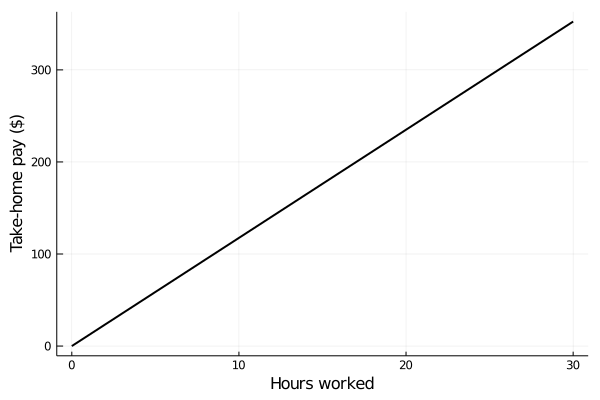
\includegraphics[width=0.45\textwidth]{linear.png}
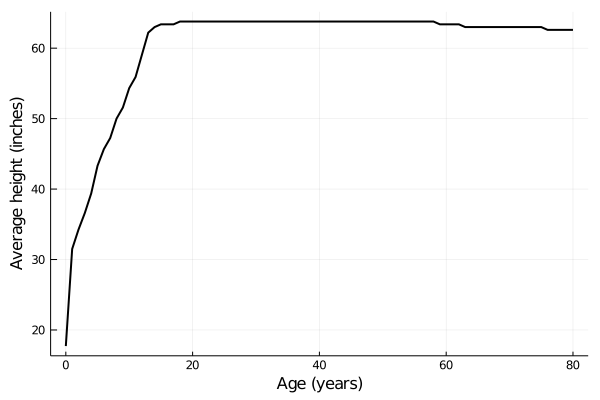
\includegraphics[width=0.45\textwidth]{nonlinear.png}
\caption{Linear and non-linear functions.}
\label{fig:linearNLPlots}
\end{figure}

By contrast, suppose I wanted to predict how tall a typical American human
female would be based on her age. While it's true that for most age ranges the
two variables increase together (just as more hours-worked implies more
take-home pay, so does more years-on-earth implies more inches-off-the-ground),
the plot is no longer a straight line (see the right side of
Figure~\ref{fig:linearNLPlots}).

It's worth lingering for a moment on what linear \textit{means} and how it
colors our assumptions about what to expect. Imagine this conversation:

\begin{dialogue}

\speak{You} Hey boss, I know I'm normally only scheduled to work for 12 hours a
week, and I get 120 bucks for that. But I need to start saving up for a plane
ticket to see my grandparents, so I'd like to inch that up to 15 hours next
week. That okay?

\speak{Boss} Sure, you can do 15 next week. That'll make your take-home
pay an even \$5,000 for the week.

\speak{You} \direct{Jaw drops open} Whoa, five \textit{grand}?! Heck, in that
case, push me up to 20 -- I can make some headway on my fall tuition!

\speak{Boss} Twenty hours it is -- you'll earn a total of 75\textcent~for
that.

\speak{You} \textit{D'oh!!}

\end{dialogue}

The above dialogue is absurd. But exactly \textit{why} is it absurd? Answer:
because we expect weekly-pay-vs.-hours-worked to be linear, and the values
given in the dialogue violate our linear assumptions.

\bigskip
The following scene, by contrast, \textit{isn't} absurd:

\begin{dialogue}

\speak{You} It's now been 12 months since I bought it, and my Blackberry stock
is currently worth \$120. Dear Crystal Ball, how much will it be worth three
months from now (the 15-month point)?

\speak{Crystal Ball} Blackberry will skyrocket in the public's imagination
three months from now, so at the 15-month mark your stock will be valued at
\$5,000.

\speak{You} Woo-hoo! And how about at the 20-month mark?

\speak{Crystal Ball} Unfortunately for shareholders, Blackberry Inc.~will make
some bad business decisions and crash. The stock will be nearly worthless --
just 75\textcent.

\speak{You} Yikes -- glad I asked! Please sell it in three months, okay?

\end{dialogue}

This scenario doesn't seem out of the question because we have no expectations
about stock prices being linear in time.

\medskip

So what exactly are those linear expectations? If you work it out, they come
down to two:

\definecolor{shadecolor}{rgb}{.9,.9,.9}
\begin{framed}
If a function $f(x)$ is linear, then:
\begin{compactitem}
\item $f(a\cdot x)$ is always simply $a\cdot f(x)$.
\item $f(x+y)$ is always simply $f(x)+f(y)$.
\end{compactitem}
\end{framed}

Take the first one. Let's say Wawa is selling a King Size Kit Kat bar for
\$1.50. How much would four bars cost? The answer's got to be \$6.00. It would
be weird to be anything else. In this example, if $x$ is the number of Kit Kat
bars, and $f(x)$ is the total cost. $f(x) = 1.5x$, and predictably, $f(4\cdot
1) = 4 \cdot f(1) = 4 \cdot 1.5 = 6.$

For the second rule, let's say we bought two Kit Kat bars today and three more
tomorrow. How much for the total? If the universe is working normally, buying
two today and three tomorrow would be the same price as buying five altogether.
And it's true: $f(2+3) = f(2) + f(3) = 3 + 4.5 = 7.5 = f(5)$. It would be weird
to work any other way.

When we have non-linear functions, we don't expect these things to be true. If
my nine-year old daughter is 4 feet tall, I don't expect her to be 8 feet tall
when she turns eighteen. $f(a\cdot x) \neq a\cdot f(x)$. And if my Blackberry
stock is worth \$5,000 after sixteen months and \$100 after the company's
disastrous seventeenth, we don't count on it being worth \$5,100 after 33
months. $f(x+y) \neq f(x)+f(y)$.

For the rest of this entire book, the two assumptions above will always be
true. It may seem limiting, but as we've seen, there are lots of cases where it
simply doesn't make any sense for our function \textit{not} to be linear.

\section{This book contains only elephants}

\index{elephants}
\index{Ulam, Stanis\l{}aw}

The great mathematician and computational scientist Stanis\l{}aw Ulam once
quipped that dividing functions into linear and non-linear is like dividing
zoology into ``elephant'' and ``non-elephant.'' In a way it's true, because
there are certainly far more functions that \textit{don't} obey the above two
properties than there are those that do. By the same token, though, there are
far more pay schemes we could invent than just ``a regular hourly rate.'' But
hourly rates come up very, very often, and when they do, there's a lot of
amazingly useful things we can do with them. Join us on our hike and you'll
see.



% TODO: appendix with Python

% TODO: somewhere in this chapter, I should do the parachute illustration with
% the gravitational force and the cross-wind force and the momentum from the
% airplane force. But where?

% TODO: introduce the notation R^3 for a 3-dimensional vector of reals. (Note:
% I do talk about this in linearTrans chapter, so forward/backward reference
% from there.)

\chapter{Vectors}

\index{vector}
As I stated on p.~\pageref{mathematicalObject}, every ``algebra'' is comprised
of a set of mathematical objects which you can combine with various operations.
In linear algebra, those building blocks are \textbf{vector}s and
\textbf{matrices} (singular: matrix). Buried within them are many mysteries.
We'll cover them in considerable detail in this chapter and the next.

\section{Vector vs.~scalar quantities}

\index{scalar}
\index{scale of measure}

The first thing we should do is perhaps distinguish between a vector quantity
and a \textbf{scalar quantity}, which probably had the spotlight in most of
your previous math classes. A scalar value is simply a \textit{single} number,
like 5, or -3.2, or $\pi$, or even $9 + 2i$ if you're into imaginary numbers.
The word \textit{scalar} is related to the word \textit{scale}, as in a ``scale
of measure.'' Think of stepping on a scale to weigh yourself in the morning:
your scale gives you back a single number (which you may or may not like; I
won't judge).

\index{one-dimensional quantity}
\index{dimension}

We'll call scalars \textbf{one-dimensional} values. That might seem odd, since
we haven't really talked about ``dimensions,'' yet. But think of the plain-old
\textbf{number line} you learned about back in elementary school. Zero's drawn
in the middle, positive numbers to the right and negative numbers to the left,
and the whole thing extends infinitely in just one direction\footnote{It might
seem like ``two directions,'' since the number line goes both to the left and
to the right. But since \index{left-ness} \index{right-ness} left-ness is the
exact opposite of right-ness, these are considered ``the same direction''; it's
just a matter of how far you go back or forth you go along that one straight
path.}.

% TODO: draw number line

\index{tuna fish}
\index{stock price}

Examples are so ubiquitous they're hardly worth mentioning. A person's weight
in the morning is a scalar. A company's stock price on a given day is a scalar.
So is the net \textit{movement} (up or down) of a stock's price from one day to
the next. So is a respondent's answer to the survey question ``on a 1-to-10
scale, how much do you enjoy tuna fish?'' You can think of countless others.

We of course often use variables to represent scalar quantities, and in this
book we'll put a variable in italics (like ``\textit{x}'' or
``\textit{price}'') to signify that its underlying value is a scalar quantity.

\subsection{A vector: a multi-dimensional quantity}
\index{vector}

Now a vector quantity is kind of the same thing, except that it represents
\textit{more than one} value. Suppose we wanted to represent not just a stock's
price on a given day, but an entire year's worth of prices on consecutive days.
Then, we would need a vector quantity. Instead of a survey respondent's answer
to just one question, we might want to store her entire set of answers to all
twenty questions on the survey. Instead of tracking just my weight, I might
want to record my weight, height, BMI (body-mass index), and pulse, all at a
given moment.

\index{losing information}
\index{information loss}

Vectors are \textbf{multi-dimensional} quantities. And they can't be
represented on a number line. Let's say my weight is 210 lbs.~and my height is
6'2", or 74 inches. (This is not theoretical.) I could of course draw a number
line and put a dot at 74 and another dot at 210, but this wouldn't fully
represent the fact that my weight was 210 and my height was 74. For one thing,
the numbers are on completely different scales. (There's that word ``scale''
again.) For another, it's not clear which is which -- is the right-most point
supposed to be my height, or my weight? Trying to squeeze a two-dimensional
quantity into a one-dimensional number line would \textbf{lose information.}
We need a representation scheme that can accommodate the complexity of our
quantity.

\index{Cartesian plane}
\index{coordinate plane}

For a two-dimensional quantity like weight-and-height, the obvious choice is
the two-dimensional Cartesian plane. I've drawn the vector with my height and
weight on the left side of Figure~\ref{fig:vector}. You'll see that there's an
\textit{arrow} from the origin to the point (210,74), rather than just a
circular dot at that point, as you might have expected. This is because
sometimes, it turns out, we want to treat a vector as ``a net movement in a
particular direction for a particular distance.''


\begin{figure}[ht]
\centering
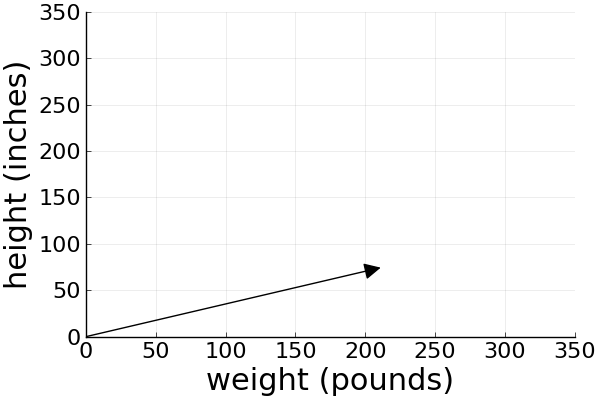
\includegraphics[width=0.4\textwidth]{vector.png}
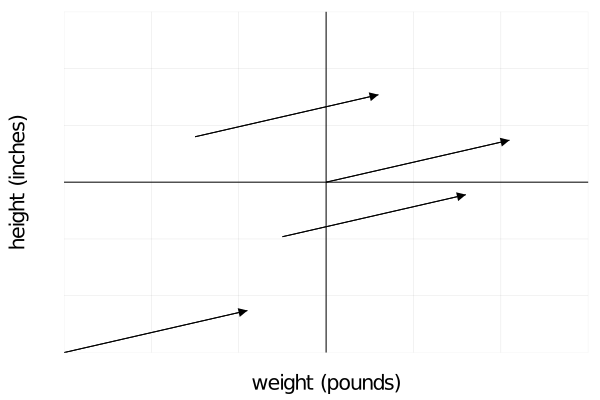
\includegraphics[width=0.58\textwidth]{vectors.png}
\caption{Left: a two-dimensional vector, depicted in a Cartesian plane. Right:
several copies of \textit{the same vector}, shown originating at various
points. They're considered ``the same'' vector because they all go in the same
direction and have the same length; the point they start at is irrelevant.}
\label{fig:vector}
\end{figure}

\index{magnitude (of a vector)}
\index{length (of a vector)}
\index{point of origin}
\index{direction (of a vector)}
\index{tail (of a vector)}
\index{tip (of a vector)}
\index{Stark, Arya}

You can see this illustrated on the right-hand side figure, where I've drawn
several copies of \textit{the same vector}. This may seem weird, but in terms
of pictures, here's how you want to think of it: \textbf{a vector has a
direction and a magnitude, but not a starting point}. The direction is the
specific angle in which it points, and (for now) we use the word
``\textbf{magnitude}'' to mean how long the vector is from its \textbf{tail} to
its \textbf{tip}. (As Arya Stark would say, the tip is the ``pointy end'' with
the arrowhead.) Curiously, there are alternative ways of judging the length, or
magnitude, of a vector, which we'll revisit in section~\ref{sec:norms}.

\index{counter-clockwise}

In the case of Stephen's biometric vector, its direction is
east-by-northeast-ish (about 19.4\textdegree\ counter-clockwise from the
$x$-axis) and its magnitude is 222.6. But it doesn't have any intrinsic ``point
of origin''; it's just an arrow pointing this-a-way and yea-far, no matter
where it might be anchored.

\index{mosquito}

Interestingly, the word \textit{vector} comes from a root meaning ``to carry.''
You may have heard people describe mosquitoes as being ``vectors'' for a
particular disease -- this means that they carry that disease. By thinking of a
vector as an arrow like in Figure~\ref{fig:vector}, the ``carry''
interpretation might start to make sense. A vector can represent a
transposition from one point to another. If I grew 74 inches taller and gained
210 more pounds, my point on the Cartesian plane would move in the direction
and the distance of that arrow.

\subsection{Don't visualize this}

Now that was all for \textit{two} dimensions. What about vectors with three, or
five, or even twenty dimensions? Well, for the three-dimensional case you can
indeed draw a 3-d figure with three axes, and plot three-dimensional points on
it. It turns out that most humans, though, are positively horrible at
interpreting such plots. And when you move beyond three dimensions, it's
utterly hopeless. (A friend of mine in fourth grade claimed he could visualize
four dimensions in his head, but I didn't believe him and still don't.)

But importantly, that doesn't mean we won't ever deal with higher-dimensional
vectors. In fact, vectors with lots and lots of dimensions will come up
constantly for us in this book -- believe it or not, we'll do an example where
the vectors have 50,000 dimensions! :-O

Don't worry; this won't make your head explode. In fact, it's a lot easier than
you might think to work with very high-dimensional vectors. Consider the
example I gave above about tracking a company's stock price every day for a
year. That's just a list of 365 numbers, all in a row. How hard is that to
imagine?

To work with vectors of more than three dimensions, you only have to do one
thing: give up trying to visualize them in a geometric space. As I'll describe
in the next section, it only occasionally makes sense to think about vectors
geometrically anyway; much of the time, we'll simply think of them as
quantities that have more than one component, unlike their simple brethren the
scalars.

\smallskip

Finally, the notation we'll use for vector variables. Instead of putting the
variable name in italics, we'll put it in bold-face with an arrow on the top of
it, like this: $\overrightarrow{\textbf{x}}$. The individual components of the
vector will be listed in boxies (square-brackets) like this: $[\ -2\ \ 5.9\ \
17\ \ -3\ ]$. So, if we define $\overrightarrow{\textbf{stephen}}$ as the
vector with my height and weight in it, we would write:

\vspace{-.15in}

\begin{align*}
\overrightarrow{\textbf{stephen}} = [\ 210\ \ 74 \ ].
\end{align*}

\medskip

\section{Five ways to think about vectors}

\begin{figure}[ht]
\centering
\includegraphics[width=1\textwidth]{fiveWays.pdf}
\caption{Five ways to think about a vector.}
\label{fig:fiveWays}
\end{figure}


In the mathematical writings you'll encounter, computer scientists use the word
``vector'' in a variety of ways. They're all ultimately compatible with each
other, but they can seem disorientingly different at first. Really, it's a
tribute to how powerful the vector concept is that people use them in so many
ways for so many different things.

I'm going to suggest that there are \textit{five} different ways to think about
a vector, and I'm going to arrange these ways on a continuum from ``concrete''
to ``abstract.'' This spectrum is depicted in Figure~\ref{fig:fiveWays}.

Let's take it from the bottom.

\subsection{1. A sequence of two coordinates}

\index{coordinate}
\index{element}
This is the height-weight example, in which something like
$\overrightarrow{\textbf{stephen}}$ is an ordered pair that can easily be
visualized on a two-dimensional Cartesian plane. Because of this plotting
aspect, I'll often call the two parts of the vector \textbf{coordinates}, but
as we create vectors with more pieces I'll more often call them
\textbf{elements}. These terms mean the same thing -- they both refer to the
individual components of the vector.

\index{index number}

We will need a way to select one of the coordinates individually, and for that
we use an \textbf{index number} (sometimes abbreviated to simply
``\textbf{index},'' the plural of which is ``indices.'') As you can see in
Figure~\ref{fig:fiveWays}, I've put two smaller numbers directly below the two
coordinates of the bottom vector, to indicate that we call them ``coordinate
\#0'' and ``coordinate \#1.'' We'll also use the phrase ``\textbf{index into
the vector},'' where ``index'' is a verb. If we take that bottom-most vector,
and index into it at coordinate 1, we get the (scalar) value 93.

Notation-wise, if we have a two-dimensional vector called
$\overrightarrow{\textbf{bob}}$, we'll often write $bob_0$ for the value of the
first coordinate and $bob_1$ for the second.

As an aside, you might wonder why the coordinates are numbered 0 and 1 instead
of 1 and 2. The answer has to do with the fact that we'll be using Python in
this book. Every programming language has a way of indexing into its
vector-like objects, and Python, Java, and C++ all begin indexing with the
number 0. There are actually some good reasons for this, which I won't get
into. It's not universally embraced, however; languages like R and Julia start
their indexing at 1. Go figure.

\index{tail (of a vector)}
\index{tip (of a vector)}
\index{radius@``radius''}
\index{Pythagorean Theorem}
\index{crow-flies distance@``crow-flies'' distance}

Geometrically, we can compute a vector's direction and magnitude using
trigonometry. Figure~\ref{fig:directionMag} shows a vector
$\overrightarrow{\textbf{v}} = [\ 9 \ \ 21\ ]$ pictorially. Its $0^\text{th}$
coordinate (a.k.a. $v_0$) is 9, measured on the $x$-axis, and $v_1$ is 21.
Traditionally, a two-dimensional vector's magnitude is called $r$ (for
``radius,'' I believe, although don't think about that too hard) and its
direction is called $\theta$ (``theta''). The magnitude is just the crow-flies
distance from the vector's \textbf{tail} to its \textbf{tip} (computed using
the Pythagorean Theorem) and the direction is the arctangent of the
rise-over-run. In equations:

\vspace{-.25in}
\begin{align*}
r &= \sqrt{v_0^2 + v_1^2} \\
\theta &= \tan^{-1} \frac{v_1}{v_0} \\
\end{align*}
\vspace{-.55in}

\begin{figure}[ht]
\centering
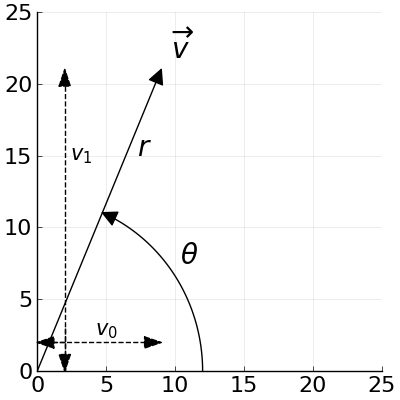
\includegraphics[width=.7\textwidth]{directionMag.png}
\caption[.]{The direction ($\theta$) and magnitude ($r$) of the vector
$\overrightarrow{\textbf{v}} = [\ 9 \ \ 21\ ]$. The direction $\theta$ is the
angle that $\overrightarrow{\textbf{v}}$ makes counter-clockwise with the
$x$-axis, and the magnitude is the length of the line.}
\label{fig:directionMag}
\end{figure}
\smallskip

\index{polar coordinates}
\index{Cartesian coordinates}

In this case, $r$ works out to 22.8 and $\theta$ is 66.8\textdegree. Think
about this, too: if, instead of giving you the values of $v_0$ and $v_1$, I
instead gave you the values of $r$ and $\theta$, you'd still have \textit{all
the information about the vector}, just in a different form. We sometimes call
$r$ and $\theta$ the \textbf{polar coordinates} of a vector, and $v_0$ and
$v_1$ the \textbf{Cartesian coordinates}. The polar coordinates are usually
written as ``$22.8 \measuredangle 66.8$\textdegree,'' which is the same vector
as $[\ 9 \ \ 21 \ ]$, just written in a different way.

Anyway, I put this way of thinking about vectors at the extreme ``concrete''
end of the spectrum, because it's so nuts-and-bolts and easy to visualize. As
we ascend up the hierarchy, things will get less and less visualizable.


\subsection{2. A sequence of more than two coordinates}

As I mentioned earlier in this chapter, having more than two coordinates in a
vector isn't really all that weird...you simply have to give up any hope of
visualizing it geometrically. But it's easy enough to do: a list of four
numbers -- 89, 93, 70, and 133 -- is the most natural thing in the world. One
could imagine finding the sum of the elements, the maximum element, the number
of negative elements, or other more exotic things.

Again, our indexing starts at 0, and this time goes up to 3. Note what this
implies: if we have a vector with four elements, there is no element \#4! This
is a common pitfall for newcomers to the subject and to languages like Python.
If I have a vector with $n$ coordinates, those coordinates are numbered 0 up to 
$n-1$, but \textit{not} up to $n$.

\index{dimension}
Also note that the number of elements/coordinates is also the
\textbf{dimensionality} (number of dimensions) of the vector. Simply put, a
vector that has nine elements in it is called ``a 9-dimensional vector.''

\subsection{3. A collection with non-numeric indices}

At this point of the hierarchy, I change my nomenclature from ``sequence'' to
``collection.'' That's because here, we don't \textit{number} the elements of
our vector anymore but instead \textit{name} them. Thus there isn't any
meaningful order to the elements anymore -- instead of ``IQ \#0,'' ``IQ \#1,''
and so forth, we have ``Jezebel's IQ,'' ``Filbert's IQ,'' and the like. Nothing
super weird here, but things may be starting to look less and less math-y to
you.

\index{label}

I'll sometimes call the names of the elements \textbf{label}s.

% TODO: talk about how diff languages represent this in diff ways; with R, you
% can name the elements of a vector, whereas in Python, you'll need a dict.

\subsection{4. A collection with non-numeric elements}

And heck, if the indices don't have to be numbers, why would the elements need
to be? And indeed we will often have cause to work with vectors like the one in
step 4 of the hierarchy (Figure~\ref{fig:fiveWays}, p.~\pageref{fig:fiveWays}),
in which there's not a number in sight. This example holds the favorite colors
for each of our four friends, which are of course non-numeric.

\subsection{5. Just a ``thing''}

Finally, you won't see this usage of vectors until you get to some more
advanced math, but I'd be doing you a disservice if I didn't point it out here.
I remember the first time I read some research in which the author was going on
and on about ``vectors,'' and I was dreadfully confused because none of his
``vectors'' seemed to have any elements in them! I was like, ``what do you mean
\textit{vectors}, dude? Did your word processor auto-correct a different
word?''

\index{vector space}
\index{algebra@``an algebra''}

This computer scientist was treating ``vectors'' as whole objects, not even
considering what their elements were (or whether they even \textit{had} any
elements). He was working with an abstract notion called a \label{vectorSpace}
\textbf{vector space} which we'll touch on next chapter; for now I'll just tell
you that it's closely related to the notion of an algebra that we discussed in
Chapter~\ref{ch:intro}. He was taking advantage of some of the elegant results
presented later in this book, which are guaranteed to hold for whatever
mathematical objects you care to define, as long as you obey certain ground
rules -- whether those objects have any ``elements'' to them or not. I mention
this mostly to anchor your future self in solid ground the first time you
inevitably come across the use of ``vector'' as a very un-list-like thing.
You'll remember reading this, say to yourself ``ah yes -- Stephen warned me
once that the extreme abstract end of the continuum works like this,'' and
proceed with confidence. I won't say anything more about it in this book.

\section{And a vector is also a function}

\index{function}
\label{vectorIsFunction}

Oh, and yet another way to think of vectors: as \textbf{function}s. We'll talk
about vectors as inputs to functions later in this book. But it's worth
recognizing at this point that a vector itself essentially \textit{is} a
function.

\index{domain}
\index{codomain}

You'll remember from Chapter 3 of \textit{Cool, Brisk Walk} that a function is
a mapping from a set of inputs to a set of outputs. Each member of the input
set (a.k.a. the ``domain'') is assigned a member of the output set
(``codomain'') as its value. (No member of the domain can be assigned to more
than one member of the codomain, but the reverse is not a constraint: multiple
members of the domain \textit{can} be assigned to the same member of the
codomain.)

Now consider this vector:

\begin{center}
\begin{tabular}{ccccccc}
$\overrightarrow{\textbf{x}} = [$ & 45 & -12 & 9 & 45 & 0 & $]$ \\
& \scriptsize{0} & \scriptsize{1} & \scriptsize{2} & \scriptsize{3} & \scriptsize{4}& \\
\normalsize
\end{tabular}
\end{center}
\vspace{-.15in}

It's a sequence of numbered elements, sure. But couldn't it just as easily be
interpreted as a function from index numbers to values? (See
Figure~\ref{vectorFunction1}.)

\begin{figure}[ht]
\centering
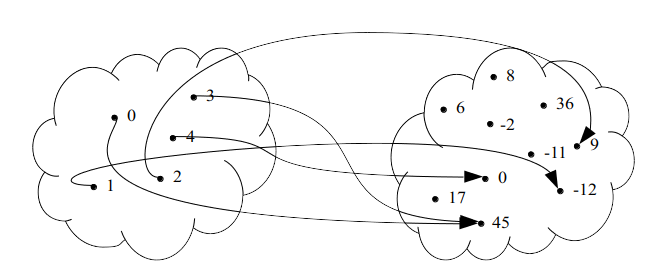
\includegraphics[width=1\textwidth]{vectorFunction1.png}
\caption[.]{The vector $\overrightarrow{\textbf{x}}$, interpreted as a function.}
\label{vectorFunction1}
\end{figure}

In function syntax, $\overrightarrow{\textbf{x}}(0) = 45$,
$\overrightarrow{\textbf{x}}(1) = -12$, $\overrightarrow{\textbf{x}}(3) = 45$,
and so on. It makes even more sense with a non-numeric vector like the
``favorite color'' example (Fig.~\ref{fig:fiveWays}), where
$\overrightarrow{\textbf{faveColor}}(\textrm{Biff}) = \textrm{blue}$ and
$\overrightarrow{\textbf{faveColor}}(\textrm{Betty Lou}) = \textrm{purple}$.
Instead of index numbers, the function's domain is comprised of the vector's
labels.

\index{ah-ha@``ah-ha"!''~moment}
\index{dictionary}
\index{hash table}
\index{array}
\index{associative array}
\index{list}
\index{vector}
\index{function}

I remember having a real ``ah-ha!''~moment the day I first realized that
vectors (called ``arrays'' or ``lists'' in some programming languages) were
really the same as key/value-pair-based associative arrays (also called
``dictionaries'' or ``hash tables'') with \textit{an index number as the key}.
Later, I had another ``ah-ha!''~and realized that both were equivalent to
functions as well, if you viewed the keys/indices as the function's domain and
the elements as the codomain. Wow. Sometimes it seems like the universe is
really all just one thing.

%Vectors in the wild
%
%
%time series
%
%temperatures over time
%
%
%
%items with attributes
%
%loan attributes: age, credit score, loan amount, salary
%
%
%
%MP3 file
%
%everything has to be in binary to be in a computer
%
%air displacement vs. time
%
%sampling
%
%
%
%image files
%
%BW vs color
%
%can do finding faces, brighten the image, whatever
%
%
%
%binary string of text
%
%plain-text, encrypt with key, to get cipher text
%
%
%
%
%Google, vector representation of web pages
%
%bag of words
%
%
%
%Emails, spam detectors
%
%
%
%matchmaker.com 
%
%
%
%Facebook:
%represent each vertex as a vector of people-he's-friends-with 
%
%
%Purchasing patterns, 
%recommender systems (collaborative filbert)
%
%
%
%system state, population growth


\section{Vector operations}
\label{vectorOps}

We're going to be combining scalars/vectors to yield other scalars/vectors like
literally all the time. The following three operations must be mastered until
you can do them in your sleep.

\subsection{Operation \#1: Scalar-vector multiplication}

\label{scalarVectorMultiplication}

What do you think you'd get if you multiplied a scalar like 2 by a vector like
$[\ 3\ \ 0\ \ 4\ ]$? As with all mathematics, we can define this operation to
be anything we want. A reasonable guess would be to take the scalar number of
copies of the vector, like so:

\vspace{-.15in}
\begin{align*}
2 \cdot [\ 3\ \ 0\ \ 4\ ] = [\ 3\ \ 0\ \ 4\ \ 3\ \ 0\ \ 4\ ] ? \quad  \quad
\textrm{NOPE}
\end{align*}
\vspace{-.15in}

But we're not doing to define it that way. Instead, we'll multiply the scalar
by each of the vector's elements individually, to get another vector with the
same number of elements:

\vspace{-.15in}
\begin{align*}
2 \cdot [\ 3\ \ 0\ \ 4\ ] = [\ 6\ \ 0\ \ 8\ ]
\end{align*}
\vspace{-.15in}

\index{scalar-vector multiplication}

This turns out to be more useful. So in general, a scalar $a$ times a vector
$\overrightarrow{\textbf{v}}$ will be:

\vspace{-.15in}
\begin{center}
\begin{framed}
\textbf{Scalar-vector multiplication:}
\begin{align*}
a \overrightarrow{\textbf{v}} = a [\ v_0\ \ v_1\ \ \dots \ \ v_{n-1}\ ] =
[\ a \cdot v_0\ \ a \cdot v_1\ \ \dots \ \ a \cdot v_{n-1}\ ],
\end{align*}
where $n$ is the number of elements in the vector.
\end{framed}
\end{center}
\vspace{-.15in}

Interestingly, there's no such thing (in common use) as ``scalar-vector
\textit{addition}.'' In other words, if someone tried to do this:

\vspace{-.15in}
\begin{align*}
2 + [\ 3\ \ 0\ \ 4\ ] = \ ??
\end{align*}
\vspace{-.15in}

\index{no can do@``no can do''}
we're simply going to say ``no can do.''

By the way, some programming languages (including Python) do give the
programmer a convenient shorthand by allowing them to type
$2 + [\ 3\ \ 0\ \ 4\ ]$ and get the value $[\ 5\ \ 2\ \ 6\ ]$. This isn't
considered a bona fide mathematical operation, though; just a notational
convenience.

\subsection{Operation \#2: Vector addition}

Adding two vectors together, though, is a perfectly acceptable enterprise,
provided that the vectors have the same number of elements. The way we do it is
to add each pair of elements together and produce another vector of the same
number of dimensions. In other words, adding $[\ 2\ \ 9\ ]$ to $[\ 4\ \ -2\ ]$
gives us:

\vspace{-.15in}
\begin{align*}
[\ 2\ \ 9\ ] + [\ 4\ \ -2\ ] = [\ 6\ \ 7\ ],
\end{align*}
\vspace{-.15in}

and in general:

\vspace{-.15in}
\begin{center}
\begin{framed}
\textbf{Vector addition:}
\begin{align*}
\overrightarrow{\textbf{x}} + \overrightarrow{\textbf{y}} &=
[\ x_0\ \ x_1\ \ \dots \ \ x_{n-1}\ ] +
[\ y_0\ \ y_1\ \ \dots \ \ y_{n-1}\ ] \\
&= [\ x_0 + y_0\ \ x_1 + y_1\ \ \dots \ \ x_{n-1} + y_{n-1}\ ],
\end{align*}
where $n$ is the number of elements in each vector.
\end{framed}
\end{center}
\vspace{-.15in}

An important issue arises in level 3 of our Figure~\ref{fig:fiveWays} hierarchy
(p.~\pageref{fig:fiveWays}). How do we add two vectors that aren't indexed by
number? Answer: we add the elements from each vector that correspond to the
same \textit{label}. And yes, the vectors must \textit{have} exactly the same
labels in order to be legitimately added in this way; otherwise, we call the
whole thing off. So:

\index{Mrs.~Peacock}
\index{Mr.~Green}
\index{Prof.~Plum}

\begin{center}
\begin{tabular}{ccccccccc}
[ & 3 & 5 & 8 & ] \ + \ [ & 1 & -6 & 4 & ] \ = \\
& \scriptsize{peacock} & \scriptsize{green} & \scriptsize{plum} & &
\scriptsize{peacock} & \scriptsize{green} & \scriptsize{plum} & \\
\normalsize
\end{tabular}
\vspace{-.15in}
\begin{tabular}{ccccc}
[ & 4 & -1 & 12 & ], \\
& \scriptsize{peacock} & \scriptsize{green} & \scriptsize{plum} & \\
\normalsize
\end{tabular}
\end{center}
\vspace{-.15in}

and

\index{Miss Scarlet}
\index{Mrs.~White}
\index{Col.~Mustard}

\begin{center}
\begin{tabular}{ccccccccc}
[ & 2 & 1 & 4 & ] \ + \ [ & 3 & 3 & 0 & ] \ = \\
& \scriptsize{scarlet} & \scriptsize{mustard} & \scriptsize{green} & &
\scriptsize{scarlet} & \scriptsize{white} & \scriptsize{plum} & \\
\normalsize
\end{tabular}

\index{no can do@``no can do''}
\vspace{-.15in}
``no can do.''
\end{center}
\vspace{-.15in}

\index{commutative}
\index{distributive}

\medskip
You can probably tell that vector addition is \textbf{commutative}, meaning
that whether we add $\overrightarrow{\textbf{x}}$ +
$\overrightarrow{\textbf{y}}$ or $\overrightarrow{\textbf{y}}$ +
$\overrightarrow{\textbf{x}}$, we get the same answer. It's also true that
vector addition, combined with scalar-vector multiplication, is
\textbf{distributive}. This means:

\vspace{-.15in}
\begin{align*}
a (\overrightarrow{\textbf{x}} + \overrightarrow{\textbf{y}}) &=
a \overrightarrow{\textbf{x}} + a \overrightarrow{\textbf{y}}
\end{align*}
\vspace{-.15in}
and

\vspace{-.15in}
\begin{align*}
(a + b) \overrightarrow{\textbf{x}} &=
a \overrightarrow{\textbf{x}} + b \overrightarrow{\textbf{x}}
\end{align*}
\vspace{-.15in}

for any scalars $a$ and $b$ and vectors $\overrightarrow{\textbf{x}}$ and
$\overrightarrow{\textbf{y}}$. This is a useful fact to know, which we'll
sometimes rely on.

\medskip

By the way, you might wonder whether vector subtraction is a thing, and it is:
in fact it turns out to just use scalar multiplication by $-1$. So:

\vspace{-.15in}
\begin{center}
$\overrightarrow{\textbf{x}} - \overrightarrow{\textbf{y}} =
\overrightarrow{\textbf{x}} + (-1 \overrightarrow{\textbf{y}}) =$ \\
$ [\ x_0 - y_0\ \ x_1 - y_1\ \ \dots \ \ x_{n-1} - y_{n-1}\ ]$.
\end{center}

For example, $[\ 5\ \ 2\ \ 7\ ] - [\ 1\ \ 4\ \ 7\ ]$ is just $[\ 4\ \ -2\ \ 0\ ]$.

\subsection{Operation \#3: Vector multiplication (dot product)}

\label{dotProduct}
\index{dot product}
\index{cross product}

Our third and final vector operation is the least intuitive of the three; at
least, it doesn't work the way I expected it to when I first learned it. It's
most commonly called the \textbf{dot product}.\footnote{There is at least one
other type of vector multiplication in common use, which we won't need in this
book. It's called the \textbf{cross product}, and is designated by a $\times$
instead of a $\cdot$. Interestingly, although the dot product is defined for
vectors of any number of dimensions, the cross product is only defined for
vectors of exactly three dimensions. (Not 2. Not 4. Only exactly 3.) Another
curious fact is that the cross product between two vectors gives you a vector
back, not a scalar like the dot product does.}

The first thing you have to wrap your head around is the fact that \textit{two
vectors multiplied together give you a scalar.} Yeah, no cap: if you multiply
an 18-dimensional vector by another 18-dimensional vector, you get back a
single lonely number.

Operationally, what happens is that you \textit{multiply} the corresponding
elements of the two vectors together, and then \textit{add} the result. So:

\vspace{-.15in}
\begin{align*}
[\ 7\ \ 8\ ] \cdot [\ 5\ \ 1\ ] = 7\cdot 5 + 8\cdot1 = 43
\end{align*}
\vspace{-.15in}

As with vector addition, we disallow taking the dot product of two vectors with
differing numbers of elements. Also, in the case of vectors with labels instead
of index numbers, we insist that the vectors have identical labels in order to
meaningfully dot-product them.

\index{dot product}
\begin{center}
\begin{framed}
\textbf{Vector multiplication (dot product):}
\begin{align*}
\overrightarrow{\textbf{x}} \cdot \overrightarrow{\textbf{y}} &=
[\ x_0\ \ x_1\ \ \dots \ \ x_{n-1}\ ] \cdot
[\ y_0\ \ y_1\ \ \dots \ \ y_{n-1}\ ] \\
&= x_0 \cdot y_0\ + x_1 \cdot y_1\ + \dots + x_{n-1} \cdot y_{n-1},
\end{align*}
where $n$ is the number of elements in each vector.
\end{framed}
\end{center}
\vspace{-.15in}

\index{commutative}

It should be obvious to you that the dot product operation is commutative:
$\overrightarrow{\textbf{x}} \cdot \overrightarrow{\textbf{y}}$ always gives
the same result as $\overrightarrow{\textbf{y}} \cdot
\overrightarrow{\textbf{x}}$.

\subsubsection{Why?}

Okay, now to address the elephant in the living room: \textit{why} would
mathematicians define vector multiplication in this way? What's the matter with
just multiplying corresponding elements and yielding a vector answer, like we
did with vector addition?

The answer is that the dot product as defined above is incredibly useful, much
more so than pairwise-multiplication will turn out to be. In fact, it's
possibly the single most important calculation in linear algebra: all kinds of
applications and more advanced computations use it as a building block.

To see this, consider the following question. What needs to be true about two
vectors in order for them to have a large dot product?

Your first inclination might be to answer ``the individual vector entries need
to be large.'' This is sort of true...but only sort of. Consider the following
two vectors:

\vspace{-.15in}
\begin{align*}
\overrightarrow{\textbf{a}} &= [\ 95\ \ 0\ 381\  ] \\
\overrightarrow{\textbf{b}} &= [\ 0\ \ 1056\ 0\  ] \\
\end{align*}
\vspace{-.15in}

Thar's som' mighty big entries in them vectors. Surely multiplying them
together would give a large result, right? No:

\vspace{-.15in}
\begin{align*}
[\ 95\ \ 0\ 381\ ] \cdot [\ 0\ \ 1056\ 0\ ] &= \\
95 \cdot 0 + 0 \cdot 1056 + 381 \cdot 0 &= 0.
\end{align*}
\vspace{-.15in}

We get zilch. By contrast, these two wimpy-looking vectors:

\vspace{-.15in}
\begin{align*}
\overrightarrow{\textbf{c}} &= [\ 1\ \ 2\ \ 5\ ] \\
\overrightarrow{\textbf{d}} &= [\ 0\ \ 2\ \ 7\ ] \\
\end{align*}
\vspace{-.15in}

do give a fairly hefty result:

\vspace{-.15in}
\begin{align*}
[\ 1\ \ 2\ \ 5\ ] \cdot [\ 0\ \ 2\ \ 7\ ] &= \\
1 \cdot 0 + 2 \cdot 2 + 5 \cdot 7 &= 39.
\end{align*}
\vspace{-.15in}

What's going on here?

\medskip

If you stare at the above calculations, you'll hit on a deep truth which is
worth pondering at length. And that is that in order for the dot product to be
large, the vectors must not only have large entries, but be large \textit{in
the same places.}

The reason that $\overrightarrow{\textbf{a}}$ and $\overrightarrow{\textbf{b}}$
had such a stunningly low dot product is that although they had large entries,
they were completely out of sync with each other. $\overrightarrow{\textbf{a}}$
had high values precisely where $\overrightarrow{\textbf{b}}$ had low ones, and
vice versa. On the other hand, even though the individual elements of
$\overrightarrow{\textbf{c}}$ and  $\overrightarrow{\textbf{d}}$ were pretty
small, they fit together nicely: for example, $\overrightarrow{\textbf{c}}$'s
largest entry and $\overrightarrow{\textbf{d}}$'s largest entry were in the
same place (element \#2), which led to a kind of synergy.

Consider how the dot product would change if we altered
$\overrightarrow{\textbf{d}}$ to be $[\ 7\ \ 2\ \ 0\ ]$ instead of $[\ 0\ \ 2\
\ 7\ ]$:

\vspace{-.15in}
\begin{align*}
[\ 1\ \ 2\ \ 5\ ] \cdot [\ 7\ \ 2\ \ 0\ ] &= \\
1 \cdot 7 + 2 \cdot 2 + 5 \cdot 0 &= 11.
\end{align*}
\vspace{-.15in}

Dang, we dropped from 39 all the way to 11 just by reordering the entries. 

\index{Jezebel}
\index{matchmaker@\texttt{matchmaker.com}}
\label{matchmakerExample}

This ability to judge roughly ``how aligned'' two vectors are comes up all the
time. Consider a dating website. Let's say that Jezebel, a heterosexual female,
signs up for a dating service and answers the questions on a compatibility
survey. She's asked, ``on a scale of 1 to 10, how much do you like action
movies? Outdoor hikes? Candlelight dinners? Reading mystery novels?'' Suppose
her answers are the following:

\begin{center}
\begin{tabular}{cccccc}
$\overrightarrow{\textbf{jezebel}}$ = [ & 5 & 2 & 10 & 2 & ] \\
& \scriptsize{action} & \scriptsize{hiking} & \scriptsize{candlelight} &
\scriptsize{mystery} & \\
\normalsize
\end{tabular}
\end{center}
\vspace{-.15in}

\index{Filbert}
\index{Wendell}
\index{Biff}

Now there are three eligible heterosexual bachelors on this site: Biff,
Filbert, and Wendell. They also took the survey, and came up with these
responses:

\begin{center}
\begin{tabular}{cccccc}
$\overrightarrow{\textbf{biff}}$ \quad \ = [ & 10 & 10 & 1 & 1 & ] \\
& \scriptsize{action} & \scriptsize{hiking} & \scriptsize{candlelight} &
\scriptsize{mystery} & \medskip \\

$\overrightarrow{\textbf{filbert}}$ \ = [ & 6 & 2 & 8 & 4 & ] \\
& \scriptsize{action} & \scriptsize{hiking} & \scriptsize{candlelight} &
\scriptsize{mystery} & \medskip \\

$\overrightarrow{\textbf{wendell}}$ = [ & 1 & 3 & 3 & 10 & ] \\
& \scriptsize{action} & \scriptsize{hiking} & \scriptsize{candlelight} &
\scriptsize{mystery} & \\
\normalsize
\end{tabular}
\end{center}
\vspace{-.15in}

\index{matchmaker@\texttt{matchmaker.com}}
The central question that \texttt{matchmaker.com} must ask is: which of these
three young gentlemen should be recommended to Jezebel?

\smallskip

The answer lies in the dot product. Just by eyeballing the survey results, you
can probably tell that Filbert is Jezebel's best match: he has high values in
roughly the same place that she does. If we compute the dot product of Jezebel
with each of the three guys, we see that the math bears that out:

\begin{align*}
\overrightarrow{\textbf{jezebel}} \cdot \overrightarrow{\textbf{biff}} &=
5 \cdot 10 + 2 \cdot 10 + 10 \cdot 1 + 2 \cdot 1 = 82 \\
\\
\overrightarrow{\textbf{jezebel}} \cdot \overrightarrow{\textbf{filbert}} &=
5 \cdot 6 + 2 \cdot 2 + 10 \cdot 8 + 2 \cdot 4 = 122 \\
\\
\overrightarrow{\textbf{jezebel}} \cdot \overrightarrow{\textbf{wendell}} &=
5 \cdot 1 + 2 \cdot 3 + 10 \cdot 3 + 2 \cdot 10 = 61 \\
\end{align*}

Since Filbert has the highest dot product with Jezebel, Filbert's vector is in
some sense ``more closely aligned'' with hers, reflecting their similar
interests. So our website will show Filbert's pic and profile to Jezebel.

\medskip

\index{Mr.~Right}

It might occur to you that someone could ``beat the system'' here by answering
10 on all their survey questions. After all, increasing the individual entries
in a vector can't \textit{hurt} its dot product with another vector; the worst
it could do is not help matters, if the second vector has a zero there. So
let's say the insidious Mr.~Right (?) creates an account on the system, and
answers:

\begin{center}
\begin{tabular}{cccccc}
$\overrightarrow{\textbf{mrright}}$ \quad \ = [ & 10 & 10 & 10 & 10 & ] \\
& \scriptsize{action} & \scriptsize{hiking} & \scriptsize{candlelight} &
\scriptsize{mystery} & \medskip \\
\normalsize
\end{tabular}
\end{center}
\vspace{-.15in}

Pairing him with Jezebel yields:

\vspace{-.15in}
\begin{align*}
\overrightarrow{\textbf{jezebel}} \cdot \overrightarrow{\textbf{mrright}} &=
5 \cdot 10 + 2 \cdot 10 + 10 \cdot 10 + 2 \cdot 10 = 190 \\
\end{align*}
\vspace{-.25in}

which blows away the competition. Mr.~Right can have any girl he wants, whether
or not he and she are truly compatible. There's a way to fix this, which we'll
see later in this chapter (section~\ref{normalizing},
p.~\pageref{normalizing}). For now, just grasp the main point that two vectors
having large entries in the same places tends to magnify their dot product.

\bigskip
\bigskip
\phantom{.}

\subsection{Geometric interpretation}

Now let's build some \textit{geometric} intuition about the dot product.
Consider the two vectors $\overrightarrow{\textbf{a}}$ and
$\overrightarrow{\textbf{b}}$ in Figure~\ref{fig:dotproduct1}.
$\overrightarrow{\textbf{a}}$ is the vector $[\ 2\ \ 0\ ]$ and
$\overrightarrow{\textbf{b}}$ is $[\ 0\ \ 3\ ]$. What is their dot product?
$2\cdot 0 + 0\cdot 3 = $ a big fat zero.

\begin{figure}[ht]
\centering
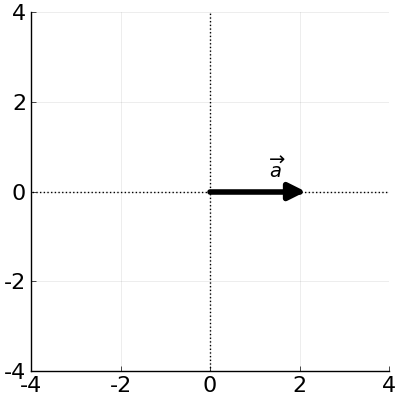
\includegraphics[width=0.45\textwidth]{dotProduct1a.png}
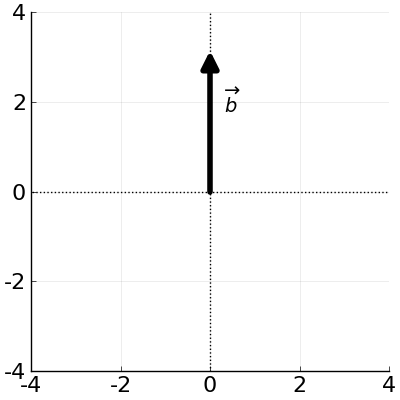
\includegraphics[width=0.45\textwidth]{dotProduct1b.png}
\caption{Two vectors whose dot product is 0.}
\label{fig:dotproduct1}
\end{figure}

\bigskip
Okay, same exercise, but now in Figure~\ref{fig:dotproduct2}. Now we have the
vectors $\overrightarrow{\textbf{a}} = [\ 3\ \ 3\ ]$ and
$\overrightarrow{\textbf{b}} = [\ -2\ \ 2\ ]$. What is their dot product? Once
more, zero: $3\cdot -2 + 3\cdot 2 = 0$.

\begin{figure}[ht]
\centering
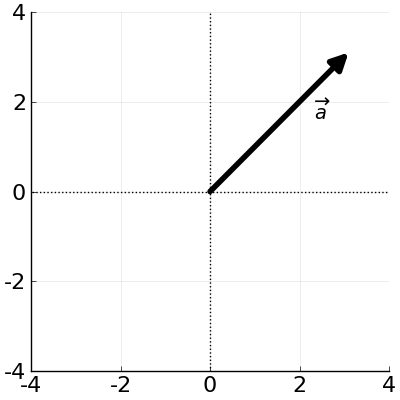
\includegraphics[width=0.45\textwidth]{dotProduct2a.png}
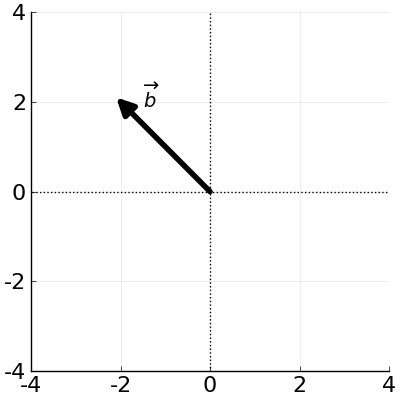
\includegraphics[width=0.45\textwidth]{dotProduct2b.png}
\caption{Another two vectors whose dot product is 0.}
\label{fig:dotproduct2}
\end{figure}

\bigskip
One more chorus. Figure~\ref{fig:dotproduct3} shows the
vectors $\overrightarrow{\textbf{a}} = [\ 1\ \ -2\ ]$ and
$\overrightarrow{\textbf{b}} = [\ -4\ \ -2\ ]$. What is their dot product? Yet
again, exactly zero: $1\cdot -4 + -2\cdot -2 = 0$.

\begin{figure}[ht]
\centering
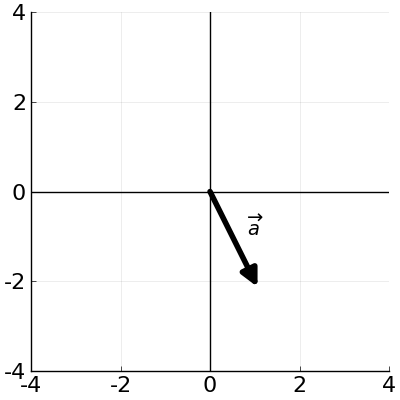
\includegraphics[width=0.40\textwidth]{dotProduct3a.png}
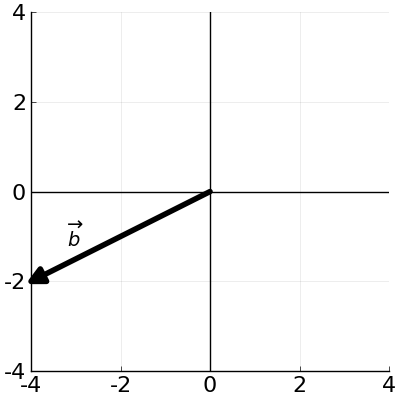
\includegraphics[width=0.40\textwidth]{dotProduct3b.png}
\caption{Yet another two vectors whose dot product is 0.}
\label{fig:dotproduct3}
\end{figure}

\bigskip

\index{perpendicular}
\index{orthogonal}
\index{right angle}

Three pairs of vectors, all of which have zero dot products. Now what's common
to all three examples? Answer: \textit{the vectors are perpendicular to each
other.} This is easier to see when we plot each pair on the same graph, as in
Figure~\ref{fig:allTogether}.

\begin{figure}[ht]
\centering
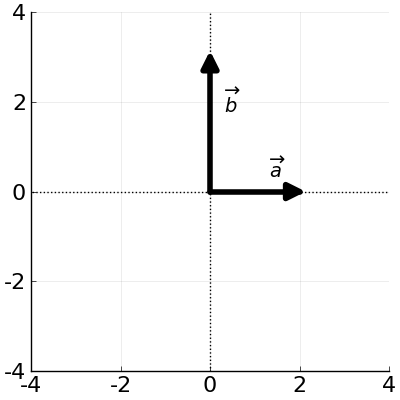
\includegraphics[width=0.31\textwidth]{dotProduct1.png}
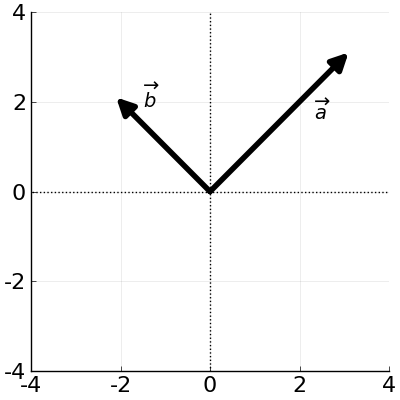
\includegraphics[width=0.31\textwidth]{dotProduct2.png}
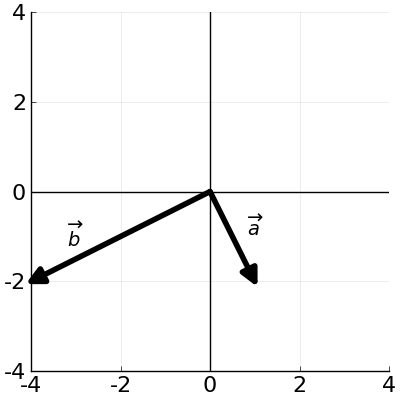
\includegraphics[width=0.31\textwidth]{dotProduct3.png}
\caption{The three pairs of vectors plotted together. The fact that they are
orthogonal to each other is what makes their dot products zero.}
\label{fig:allTogether}
\end{figure}

Whenever you have two vectors at exactly right angles to each other, their dot
product will be at a minimum; namely, zero. Our linear algebra term for this,
annoyingly, is not ``perpendicular'' (a word you already know) but
\textbf{orthogonal}. When two vectors are orthogonal, they're ``as unaligned as
possible.''

Think of it this way. Pick any of the three pairs of vectors in
Figure~\ref{fig:allTogether}, and pretend that your goal is to go in the
$\overrightarrow{\textbf{b}}$ direction. You want to get ``as b-ward as
possible.'' But suppose your only option was to go in the direction of
$\overrightarrow{\textbf{a}}$. Would you make any meaningful progress towards
your goal? The answer is no: $\overrightarrow{\textbf{a}}$ is exactly the
direction that doesn't let you move \textit{anywhere} you want to go. On the
left-most figure, for example, if your goal was to get from the origin due
north to the point $(0,15)$, you can't make any progress whatsoever if you're
allowed only to travel along the $x$-axis. And that's true for all three of
those pairs.

To get a non-zero dot product, the two vectors at least have to point
\textit{somewhat} in the same direction. Take the two in
Figure~\ref{fig:dotProduct4}, where $\overrightarrow{\textbf{a}} = [\ 3\ \ -3\
]$ and $\overrightarrow{\textbf{b}} = [\ 2\ \ -4\ ]$. These vectors are clearly
\textit{not} orthogonal, and hence their dot product is non-zero: $3\cdot 2 +
-3\cdot -4 = 18$.

\begin{figure}[ht]
\centering
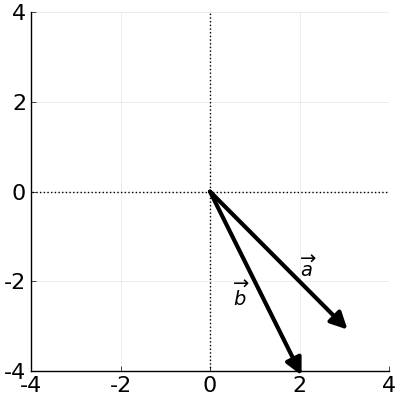
\includegraphics[width=0.80\textwidth]{dotProduct4.png}
\caption{Two \textit{non}-orthogonal vectors, whose dot product is 18.}
\label{fig:dotProduct4}
\end{figure}

In general, the more the arrows point in the same direction, the higher the dot
product, holding everything else equal. The more they diverge to right angles,
the more the dot product drops to zero. I'll have more to say about this in
Section~\ref{sec:norms} when we look at an alternate way to compute the dot
product geometrically.



\section{The vector operations in action}

This book is chock full of examples of using vectors in the real world. Let me
give one now which illustrates the eminent usefulness of these three vector
operations.

\smallskip
\label{bakeSale}
Let's say we've been tasked with baking goodies for a bake sale. There are
three recipes we're planning on making in bulk: chocolate chippers (my personal
fave), brownies, and fudge. Upon consulting our recipe book, we write down an
ingredient list for each:

\index{bake sale}
\index{brownies}
\index{fudge}
\index{chocolate chip cookies}

\begin{center}
\begin{tabular}{ccccccc}
$\overrightarrow{\textbf{chippers}}$ \ = [ & 2 & 1 & 1 & 1 & 3 &] \\
& \scriptsize{butter} & \scriptsize{sugar} & \scriptsize{chips} &
\scriptsize{flour} & \scriptsize{eggs} \smallskip \\
$\overrightarrow{\textbf{brownies}}$ \ = [ & 1 & 1 & 4 & 2 & 2 &] \\
& \scriptsize{butter} & \scriptsize{sugar} & \scriptsize{chips} &
\scriptsize{flour} & \scriptsize{eggs} \smallskip \\
\ \ $\overrightarrow{\textbf{fudge}}$ \quad \ = [ & 2 & 2 & 4 & 0 & 0 &]. \\
& \scriptsize{butter} & \scriptsize{sugar} & \scriptsize{chips} &
\scriptsize{flour} & \scriptsize{eggs} \bigskip \\
\end{tabular}
\end{center}
\vspace{-.05in}

This shows, for each of our five ingredients, how many ``units'' of each one is
required for one recipe's worth.\footnote{Warning: do \textit{not} attempt to
use these ingredient lists to actually make real goodies! I have left many
things out for simplicity. These would taste ratchet if you made them. Consult
a real recipe book.} Chocolate chip cookies evidently require two sticks of
butter, one cup of sugar, one package of Ghirardelli chocolate chips,
\textit{etc.}

\medskip

Additionally, we define these two vectors:
\index{fat, saturated}
\index{saturated fat}
\index{Wegmans}
\index{shopping list}

\begin{center}
\begin{tabular}{ccccccc}
$\overrightarrow{\textbf{wegmans}}$ \quad \ = [ & 1.59 & 2.79 & 3.49 & 1.67 &
.4 &] \\
& \scriptsize{butter} & \scriptsize{sugar} & \scriptsize{chips} &
\scriptsize{flour} & \scriptsize{eggs} \medskip \\
$\overrightarrow{\textbf{satfat}}$ \quad \ = [ & 56 & 0 & 24 & 1 & 1.6 &] \\
& \scriptsize{butter} & \scriptsize{sugar} & \scriptsize{chips} &
\scriptsize{flour} & \scriptsize{eggs} \medskip \\
\normalsize
\end{tabular}
\end{center}
\vspace{-.15in}

The first shows how much each of these ingredients is currently selling for at
Wegmans. For the health-conscious, the second shows how many grams of
saturated fat is present in each unit of the various ingredients. (*shudder*)

\medskip
Now, let's consider some common questions we might need to answer:

\begin{enumerate}
\itemsep1.5em
\item ``If we want to bake five batches of chocolate chippers for our bake sale,
what's on our shopping list?''

The answer is a simple vector operation:

% TODO: make this not look ratchet:

\vspace{.2in}
$\overrightarrow{\textbf{shoppinglist}}$ = 5 
$\overrightarrow{\textbf{chippers}}$
\vspace{-.15in}
\begin{center}
\begin{tabular}{rlcccccc}
&\quad\quad= [ & 10 & 5 & 5 & 5 & 15 &] \\
&& \scriptsize{butter} & \scriptsize{sugar} & \scriptsize{chips} &
\scriptsize{flour} & \scriptsize{eggs} & \smallskip \\
\end{tabular}
\end{center}

Scalar-vector multiplication gives us exactly what we want: multiply the number
of recipes by each ingredient's per-recipe quantity.

\item ``We've decided on six recipes of brownies and fudge, plus a dozen
batches of chocolate chippers. What's on our shopping list?''
\label{shoppingListQuestion}

Putting vector addition into the mix (see what I did there?) gives us our
elegant answer:

\begin{center}
$\overrightarrow{\textbf{shoppinglist}}$ 
= 6 $\overrightarrow{\textbf{brownies}}$
+ 6 $\overrightarrow{\textbf{fudge}}$
+ 12 $\overrightarrow{\textbf{chippers}}$

\begin{tabular}{rlcccccc}
&\quad\quad\quad\quad  = [ & 42 & 30 & 60 & 24 & 48 &] \\
&& \scriptsize{butter} & \scriptsize{sugar} & \scriptsize{chips} &
\scriptsize{flour} & \scriptsize{eggs} & \smallskip \\
\end{tabular}
\end{center}

\item ``My recipe tells me there are 16 brownies in a batch. How much saturated
fat is in each brownie?''

\index{dot product}

Here's where the dot product comes in handy. We have a vector
($\overrightarrow{\textbf{brownies}}$) that gives us the amount of each
ingredient, and another ($\overrightarrow{\textbf{satfat}}$) that gives us
per-unit fat content. The dot product is just what we need: multiply each
ingredient amount by its fat content, and add up the results. It's a snap! All
we then need to do is find the per-serving total by taking only a sixteenth of
a batch, which is scalar-vector multiplication again. Putting it all together:

\begin{align*}
\textit{fatPerBrownie} &=
\frac{1}{16} (\overrightarrow{\textbf{brownies}} \cdot
\overrightarrow{\textbf{satfat}}) \\[10pt]
&= \frac{1}{16} (1\cdot 56 + 1\cdot 0 + 4\cdot 24 + 2\cdot 1 + 2\cdot 1.6)
\smallskip \\[10pt]
&= 9.825\  \textrm{grams}.
\end{align*}

Ouch. Better sneak just one of those.

\item Finally, ``how much is this all going to cost me at Wegmans?''

We already computed the grand shopping list in
question~\ref{shoppingListQuestion}, above. To get the cost of this list, we
again simply use the dot product:

\begin{align*}
\textit{totalCost} &=
\overrightarrow{\textbf{shoppinglist}} \cdot
\overrightarrow{\textbf{wegmans}} \\[5pt]
&= 42\cdot 1.59 + 30\cdot 2.79 + 60\cdot 3.49 + 24\cdot 1.67 + 48\cdot .4
\smallskip \\[5pt]
&= \$419.16.
\end{align*}

Wowza: I sure hope we sell all these!

\end{enumerate}

Hopefully this gives you a feel for why the three operations -- and especially
the dot product -- are eminently useful. They turn out to be exactly what we
want to do with vectors much of the time, which is why they were invented. Get
to know them intimately.

\section{More about magnitude}
\label{sec:norms}

\index{tip (of a vector)}
\index{tail (of a vector)}
\index{Pythagorean Theorem}
\index{Euclidean distance}
\index{crow-flies distance@``crow-flies'' distance}

Flip for a moment back to Figure~\ref{fig:directionMag} on
p.~\pageref{fig:directionMag}. You'll recall that we defined the ``magnitude''
of the $\overrightarrow{\textbf{v}}$ vector as $r$: the crow-flies distance
from its tail to its tip, as computed by the Pythagorean Theorem. In that case,
we computed $r = \sqrt{v_0^2 + v_1^2} = 22.8$ for
$\overrightarrow{\textbf{v}}$'s magnitude.

Now like all of mathematics, we can define things however we want. It turns out
that this crow-flies distance thing -- also called the \textbf{Euclidean
distance} after Euclid, the ancient Greek geometer -- is only one possible way
to define the ``length'' or ``magnitude'' of a vector. This section includes
several others which prove useful in various settings.

\index{norm (of a vector)}
% TODO: put notation in index
\index{double-pipe sign@double-pipe sign ($\norm{\cdot}$)}

Oh, and before we get started, here's yet another piece of verbiage. The
preferred mathematical term for the sort of generalized magnitude measurement
presented below is the ``\textbf{norm}'' of a vector. We'll define several
different norms, each of which offers a different take on measuring a vector's
``size'' or ``bigness.'' No matter how we define it, \textit{the norm of a
vector is always a scalar}. We use double-pipe signs to represent it, like
this: $\norm{\overrightarrow{\textbf{v}}}$.

\subsection{The Euclidean (``$\boldsymbol\ell^\textbf{2}$'') norm}

The most common norm is the \textbf{Euclidean norm}, which is just what we
covered on p.~\pageref{fig:directionMag}. The Pythagorean Theorem is your
friend.

\index{cosine}
\index{dot product}

% TODO: talk more about cosine, even show a cosine curve

The Euclidean norm is used for many, many things, one of which is a second,
equally legitimate way to compute and to think about the dot product between
two vectors. First, recall the cosine operation from trigonometry. The cosine
of a 0\textdegree\ angle is 1, the cosine of a 90\textdegree\ angle is zero,
and in between those two extremes the cosine varies smoothly from 1 down to 0.

Now suppose we have a couple of two-dimensional vectors
$\overrightarrow{\textbf{a}}$ and $\overrightarrow{\textbf{b}}$. We'll use the
same ones from the example on p.~\pageref{fig:dotProduct4}, shown here in
Figure~\ref{fig:dotProduct4WithAngle}. To refresh your memory, the vector
$\overrightarrow{\textbf{a}}$ is $[\ 3\ \ -3\ ]$ and
$\overrightarrow{\textbf{b}}$ is $[\ 2\ \ -4\ ]$.


% TODO: add a second plot to this figure, showing two vectors with the same
% magnitudes as the existing plot, but with a bigger angle between them, and
% show how the dot product is less.
\begin{figure}[ht]
\centering
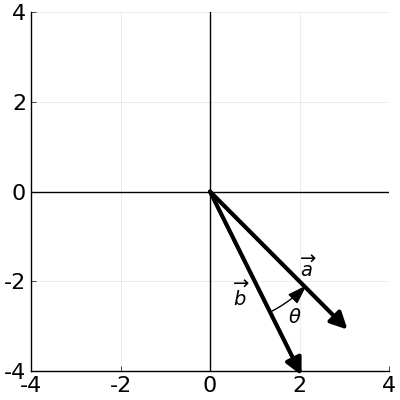
\includegraphics[width=0.6\textwidth]{dotProductWithAngle.png}
\caption{An alternate way to compute the dot product of two vectors, using the
angle between them in the calculation.}
\label{fig:dotProduct4WithAngle}
\end{figure}

We've learned that one way to compute the dot product between
$\overrightarrow{\textbf{a}}$ and $\overrightarrow{\textbf{b}}$ is to multiply
their corresponding entries:

\vspace{-.25in}
\begin{align*}
\overrightarrow{\textbf{a}} \cdot \overrightarrow{\textbf{b}} =
3\cdot2 + (-3)\cdot(-4) = 18.
\end{align*}
\vspace{-.25in}

Here's another way. We can \textit{multiply the two norms together, and then
multiply by the cosine of the angle between them.} You can really see why it's
called the dot ``product'' when you think of it this way. Multiplying vectors
is just multiplying their lengths...but there's a catch. We also multiply by
the cosine of their angle, so that the more they diverge from each other, the
lower the dot product.

In this example, we compute the angle between them (called $\theta$ in the
figure):

\vspace{-.2in}
\begin{align*}
\textrm{angle of } \overrightarrow{\textbf{a}} &= \tan^{-1} \frac{-3}{3} =
-45\degree\ \\
\textrm{angle of } \overrightarrow{\textbf{b}} &= \tan^{-1} \frac{-4}{2} =
-63.43\degree\ \\ 
\theta = \textrm{angle between } \overrightarrow{\textbf{a}} \textrm{ and }
\overrightarrow{\textbf{b}} &= -45\degree - (-63.43\degree) = 18.43\degree\ \\
\end{align*}

Now we can compute the dot product our new way:

\vspace{-.15in}
\begin{align*}
\overrightarrow{\textbf{a}} \cdot \overrightarrow{\textbf{b}} = 
\norm{\overrightarrow{\textbf{a}}} \cdot \norm{\overrightarrow{\textbf{b}}}
\cdot \cos
\theta &= \\
\sqrt{3^2+(-3)^2} \cdot \sqrt{2^2+(-4)^2} \cdot \cos 18.43\degree &= \\
4.243 \cdot 4.472 \cdot .948 & = 18. \\
\end{align*}

Yay! Same answer. I've found this a super useful way to visualize the dot
product, even though it's often more convenient to calculate it the original
way. A long vector times a long vector will give a large answer...provided
those long vectors are kinda sort pointing in the same direction. If they're
not -- and most especially, if they're at right angles to each other, a la the
Figure~\ref{fig:allTogether} examples (p.~\pageref{fig:allTogether}) -- then
the dot product can be miniscule even if the vectors themselves are long.

\bigskip

Okay, enough about the dot product. Back to the Euclidean norm itself. So far
we've been assuming two dimensions. But importantly, the Euclidean norm applies
equally well in \textit{any} number of dimensions. Suppose we had a
five-dimensional vector, like this one:

\begin{center}
$\overrightarrow{\textbf{f}} = [\ 3\ \ -4\ \ 5\ \ 17\ \ 0\ ]$.
\end{center}

The Pythagorean Theorem -- which in high school you may have only learned in a
two-dimensional setting -- still works just fine:

\begin{center}
$\norm{\overrightarrow{\textbf{f}}} =
\sqrt{3^2 + (-4)^2 + 5^2 + 17^2 + 0^2} = 18.412$.
\end{center}

Note: you still \textit{square} the entries and take the \textit{square} root
of the sum. (You don't take the fifth power of the entries and the fifth root
of the sum, like I expected when I first learned this.)

The result is (*deep breath*): ``the length of the straight line from the
origin to the point $(3,-4,5,17,0)$ in five-dimensional space.'' You can't
visualize it, so don't try. Just believe. No matter how many entries a vector
has, you can compute its crow-flies length this way.

Now for weird but ultimately consistent reasons, this Euclidean norm is also
called the ``$\ell^2$ norm''\footnote{Pronounced ``ell two,'' not ``ell
squared.''} of the vector. And we will sometimes write the 2 in as a subscript
to the double-pipe, like this:

\begin{center}
$\norm{\overrightarrow{\textbf{f}}}_2 = 18.412$.
\end{center}

I know it seems strange, but just go with it for now. And remember this, too:
if we \textit{don't} have any subscript after the $\norm{\cdot}$ signs,
\textit{the default is 2}. In other words, unless explicitly stated, the
``normal'' meaning of \textit{norm} is the $\ell^2$ norm, a.k.a. Euclidean
distance, computed by the Pythagorean Theorem.

\subsection{The Manhattan (``$\boldsymbol\ell^\textbf{1}$'') norm}

\index{Manhattan norm}
\index{taxicab norm}

% TODO: picture showing Manhattan distance and city blocks.

Imagine yourself in downtown Manhattan, New York City. You're a software
developer on an upper floor of the sleek new building at the corner of 33rd
Street and 8th Avenue. It's just about time for lunch, and you and your fellow
developers are discussing where to go -- the Thai place on 25th St.~and 10th
Ave.? The new Hungarian restaurant that opened up on 44th St.~and 6th Ave.? Or
will it be just the greasy subway shop four blocks uptown today?

One of the factors in your decision is the distance: you can't take forever for
lunch because you have a team meeting at 1:30pm. So you need to work out how
long it will take to walk (or take a taxicab) to each of these places. 

Now one (stupid) approach would be to use find the latitude and longitude of
both your office and each of the restaurants, and compute the Euclidean
distance. I say ``stupid'' because this is really only useful if you have a
helicopter. (We can dream.) In my world, you can't fly over buildings; you have
to walk around them. There's no point in computing the crow-flies distance if
you're not a crow.

So how do we determine the distance? Simple: it's just the number of blocks you
have to walk. Consider the Thai place. To get from 35th Street to 24th, we have
to walk five blocks. To get from 8th Avenue to 10th, we have to walk two.
Therefore, the walking distance between these two restaurants is ``ten
blocks.'' Note that it doesn't matter whether we walk the blocks west first and
then south, or south first and then west, or zig-zag back and forth between
streets and avenues: as long as we travel one of the shortest routes through
the buildings (which means never going east or north), it'll be ten blocks.

For reasons which should now be obvious, this way to measure distance is called
the \textbf{Manhattan norm} (or \textbf{taxicab norm}). You can measure the
Manhattan distance between two points by simply \textit{adding the absolute
value of the pairwise differences between elements.} That's easier to do than
to say. For our office-to-Thai-restaurant journey:

\vspace{-.15in}
\begin{align*}
\textrm{dist}_\textrm{Manhattan} = |33-25| + |8-10| = 8 + 2 = 10\ 
\textrm{blocks}
\end{align*}

The Euclidean distance, of course, is somewhat less:

\vspace{-.15in}
\begin{align*}
\textrm{dist}_\textrm{Euclidean} = \sqrt{(33-25)^2 + (8-10)^2} = 8.246\ 
\textrm{blocks}
\end{align*}

which is why helicopters can be useful.

When speaking of the norm of a vector, we always start at the origin and travel
out from there. The Manhattan norm of a vector $\overrightarrow{\textbf{v}}$,
which is written $\norm{\overrightarrow{\textbf{v}}}_1$, is thus: 

\begin{center}
$\norm{\overrightarrow{\textbf{v}}}_1 = |v_0| + |v_1| + \cdots + |v_{n-1}|$,
\end{center}

where $n$ is the vector's number of dimensions. For example, let's compute the
Manhattan norm of the 5-d vector $\overrightarrow{\textbf{f}}$ we previously
used (with value $[\ 3\ \ -4\ \ 5\ \ 17\ \ 0\ ]$, you'll recall):

\vspace{-.15in}
\begin{align*}
\norm{\overrightarrow{\textbf{f}}}_1 &= |3| + |-4| + |5| + |17| + |0| = 29.
\end{align*}

Quite a bit higher than the Euclidean norm of 18.412, as expected.

By the way, just as the Euclidean norm was called the $\ell^2$ norm, the
Manhattan norm is called the $\ell^1$ (``ell one'') norm. You might take a
moment to mull over why, and then see if you're right when I unveil the
explanation in the next section.

\subsection{This ``$\boldsymbol\ell^\textbf{\#}$'' business}

Okay. Here's how the Euclidean, Manhattan, and all the other norms we haven't
yet discussed are related.

First, I'm going to write the formula for the Manhattan norm in a slightly
different way. You'll probably wonder why I would complicate the expression,
but suspend your disbelief for a moment. Instead of this:

\begin{center}
$\norm{\overrightarrow{\textbf{v}}}_1 = |v_0| + |v_1| + \cdots + |v_{n-1}|$,
\end{center}

I'm going to write it this way:

\begin{center}
$\norm{\overrightarrow{\textbf{v}}}_1 = \sqrt[1]{|v_0|^1 + |v_1|^1 + \cdots +
|v_{n-1}|^1}$.
\end{center}

Wut? Yeah. First, convince yourself that I haven't actually changed anything.
Remember that any number ``to the first power'' is just the number itself. And
notice that I'm not taking the \textit{square} root here, but ``the
\textit{first} root.'' If you didn't know this, ``the first root'' of a number
is also just the number itself.

Bottom line is that these two formulas for the Manhattan norm are identical.

All right, but why do this? Here's why. Check out these two expressions, back
to back:

\vspace{-.15in}
\begin{align*}
\norm{\overrightarrow{\textbf{v}}}_1 &= \sqrt[1]{|v_0|^1 + |v_1|^1 + \cdots +
|v_{n-1}|^1} \quad \textrm{(Manhattan norm)}\\
\norm{\overrightarrow{\textbf{v}}}_2 &= \sqrt[2]{|v_0|^2 + |v_1|^2 + \cdots +
|v_{n-1}|^2} \quad \textrm{(Euclidean norm)}\\
\end{align*}

Aha. See where I'm going with this? I've slipped in absolute value signs in the
Euclidean norm elements -- but that's okay, since if you square a negative
number you get a positive result anyway. And I put a ``2'' above the root sign,
to be explicit that it's the \textit{square} root. Now the formulas are
identical except for ``1'' vs.~``2.''

And now I'm going to tell you that we can use \textit{any} number, not just 1
or 2. The others don't have special names, but they're legit nonetheless:

\vspace{-.15in}
\begin{align*}
\norm{\overrightarrow{\textbf{v}}}_1 &= \sqrt[1]{|v_0|^1 + |v_1|^1 + \cdots +
|v_{n-1}|^1} \quad \textrm{(Manhattan norm)}\\
\norm{\overrightarrow{\textbf{v}}}_2 &= \sqrt[2]{|v_0|^2 + |v_1|^2 + \cdots +
|v_{n-1}|^2} \quad \textrm{(Euclidean norm)}\\
\norm{\overrightarrow{\textbf{v}}}_3 &= \sqrt[3]{|v_0|^3 + |v_1|^3 + \cdots +
|v_{n-1}|^3} \quad \textrm{($\ell^3$ norm)}\\
\norm{\overrightarrow{\textbf{v}}}_4 &= \sqrt[4]{|v_0|^4 + |v_1|^4 + \cdots +
|v_{n-1}|^4} \quad \textrm{($\ell^4$ norm)}\\
\norm{\overrightarrow{\textbf{v}}}_5 &= \sqrt[5]{|v_0|^5 + |v_1|^5 + \cdots +
|v_{n-1}|^5} \quad \textrm{($\ell^5$ norm)}\\
& \vdots \\
\norm{\overrightarrow{\textbf{v}}}_\infty &= \sqrt[\infty]{|v_0|^\infty +
|v_1|^\infty + \cdots + |v_{n-1}|^\infty} \quad \textrm{($\ell^\infty$ norm)}\\
\end{align*}

That's right, we can even have an ``infinity norm.'' So what do all these options do?


\subsection{$\boldsymbol\ell^\textbf{3}$ and higher norms}

Let's go back to our friend $\overrightarrow{\textbf{f}}$ whose value
is $[\ 3\ \ -4\ \ 5\ \ 17\ \ 0\ ]$. We've already computed the first two norms;
let's keep going and see what happens:

\vspace{-.15in}
\begin{align*}
\norm{\overrightarrow{\textbf{f}}}_1 &= \sqrt[1]{|3|^1 + |-4|^1 + |5|^1 + |17|^1 + |0|^1} = 29\\
\norm{\overrightarrow{\textbf{f}}}_2 &= \sqrt[2]{|3|^2 + |-4|^2 + |5|^2 + |17|^2 + |0|^2} = 18.412\\
\norm{\overrightarrow{\textbf{f}}}_3 &= \sqrt[3]{|3|^3 + |-4|^3 + |5|^3 + |17|^3 + |0|^3} = 17.246\\
\norm{\overrightarrow{\textbf{f}}}_4 &= \sqrt[4]{|3|^4 + |-4|^4 + |5|^4 + |17|^4 + |0|^4} = 17.049\\
\norm{\overrightarrow{\textbf{f}}}_5 &= \sqrt[5]{|3|^5 + |-4|^5 + |5|^5 + |17|^5 + |0|^5} = 17.010\\
& \vdots \\
\norm{\overrightarrow{\textbf{f}}}_\infty &= \sqrt[\infty]{|3|^\infty + |-4|^\infty + |5|^\infty + |17|^\infty + |0|^\infty} = 17.\\
\end{align*}

It's interesting: the numbers get smaller and smaller as we increase the \# in
``$\ell^{\#}$'', and they finally converge on \textit{the highest individual
element of the vector.} Cool! $\overrightarrow{\textbf{f}}$'s highest entry was
17, and lo and behold that's what the $\ell^\infty$ norm gives us.

The method to the madness is this: the higher the norm we take of a vector, the
more that only the single largest element matters. The lower the norm we take,
the more that all the elements equally matter. Think about the Manhattan norm:
we simply added up the (absolute value of the) elements. Every element had a
chance to shine. Higher and higher norms squeeze the life out of everything
except the single highest value.

\subsection{The $\boldsymbol\ell^\textbf{0}$ norm}

Lastly, and mostly for fun, I'll throw a ``$\ell^0$'' norm in. What does the
``zero norm'' do? It's defined to be \textit{the number of non-zero elements}
in the vector. So for our friend $\overrightarrow{\textbf{f}}$, we say that
$\norm{\overrightarrow{\textbf{f}}}_0 = 4$. This is at the other extreme from the
infinity norm: now not only do all the elements count, but they count
\textit{equally}. I don't care if you're 17 or 3; as long as you're not zero
you count towards my $\ell^0$ norm.

\section{Normalizing}

\label{normalizing}
\index{normalizing (a vector)}

Finally, let me mention the concept of ``\textbf{normalizing}'' a vector. To
normalize a vector means to whack it down to size: make its length be exactly
1. We do this when we only care about a vector's \textit{direction}, not its
magnitude, and when the magnitude might actually get in the way.

First I'll tell you how to do this, and then give you an idea of why we'd want
to. The how part is easy: you just divide the vector by its norm. (We can
choose whichever norm is appropriate, often Euclidean.) Just as ``subtracting
two vectors'' meant ``multiply the second vector by $-1$ and add them,'' so
``dividing a vector by a scalar'' means ``multiply the vector by
1-over-the-scalar.''

For example, if we normalize our vector $\overrightarrow{\textbf{b}} = [\ 2\ \
-4\ ]$ from the last section, we get:

\vspace{-.15in}
\begin{align*}
\frac{\overrightarrow{\textbf{b}}}{\norm{\overrightarrow{\textbf{b}}}} =
\frac{[\ 2\ \ -4\ ]}{\norm{[\ 2\ \ -4\ ]}} =
\frac{[\ 2\ \ -4\ ]}{\sqrt{2^2 + (-4)^2}} =
\frac{[\ 2\ \ -4\ ]}{4.472} = [\ .447 \ \ -.894\ ].
\end{align*}

This is a vector that's in the same direction as $\overrightarrow{\textbf{b}}$,
but of magnitude 1. We can verify this:

\vspace{-.15in}
\begin{align*}
\textrm{angle} = \tan^{-1} \frac{-.894}{.447} = -63.43\degree, \\
\textrm{magnitude} = \sqrt{.447^2 + (-.894)^2} = 1.
\end{align*}

\index{Mr.~Right}
\index{matchmaker@\texttt{matchmaker.com}}

Okay, now why would we want to normalize a vector? Isn't throwing away the
magnitude tantamount to losing important information? Well, it depends. Let's
return to our matchmaker dating site (p.~\pageref{matchmakerExample}). You'll
recall that the odious Mr.~Right was trying to game the system by answering 10
to all the survey questions. ``Action movies? I love 'em! Hiking! Love it!
Candlelight dinners? Love 'em!...'' He figured he could be every woman's dream
match because he'd have the maximum dot product with all of them.

But if we \textit{normalize} each person's vector before taking the dot
product, we put everybody on the same playing field. Effectively, each person
has the same amount of points to ``spend'' on the various survey questions, and
giving a high answer to one question means you're essentially going to have to
give a low answer to others.

\index{Filbert}

Consider Filbert, whose answers were:

\begin{center}
\begin{tabular}{cccccc}
$\overrightarrow{\textbf{filbert}}$ \quad \ = [ & 6 & 2 & 8 & 4 & ] \\
& \scriptsize{action} & \scriptsize{hiking} & \scriptsize{candlelight} &
\scriptsize{mystery} & \medskip \\
\end{tabular}
\end{center}
\vspace{-.15in}

His norm was $\sqrt{6^2+2^2+8^2+4^2}=10.95$, so when we normalize him, we get:

\begin{center}
\begin{tabular}{cccccc}
$\frac{\overrightarrow{\textbf{filbert}}}{\norm{\overrightarrow{\textbf{filbert}}}}$
\quad \ = [ & .548 & .183 & .730 & .365 & ] \\
& \scriptsize{action} & \scriptsize{hiking} & \scriptsize{candlelight} &
\scriptsize{mystery} & \medskip \\
\end{tabular}
\end{center}
\vspace{-.15in}

Biff's norm was $\sqrt{10^2+10^2+1^2+1^2}=14.21$, so when we normalize him, we get:

\begin{center}
\begin{tabular}{cccccc}
$\frac{\overrightarrow{\textbf{biff}}}{\norm{\overrightarrow{\textbf{biff}}}}$
\quad \ = [ & .704 & .704 & .070 & .070 & ] \\
& \scriptsize{action} & \scriptsize{hiking} & \scriptsize{candlelight} &
\scriptsize{mystery} & \medskip \\
\end{tabular}
\end{center}
\vspace{-.15in}

As for Mr.~Right, he has the largest norm: $\sqrt{10^2+10^2+10^2+10^2}=20$. So
no matter how much he tries to fool the ladies with his huge answers, his
normalized version is simply:

\begin{center}
\begin{tabular}{cccccc}
$\frac{\overrightarrow{\textbf{mrright}}}{\norm{\overrightarrow{\textbf{mrright}}}}$
\quad \ = [ & .5 & .5 & .5 & .5 & ] \\
& \scriptsize{action} & \scriptsize{hiking} & \scriptsize{candlelight} &
\scriptsize{mystery} & \medskip \\
\end{tabular}
\end{center}
\vspace{-.15in}

See how that works? Your survey responses now become relative to your
\textit{other} survey responses. Answering 10 to everything is the
same as answering 5 to everything, or even 0 to everything: you're effectively
saying ``I like all these activities equally.'' The only way to \textit{truly}
say ``I really do love candlelight dinners'' is to rank candlelight dinners
higher than other activities which you admit you like less.

Using normalized versions of the vectors, let's see how each of our eligible
bachelors pairs up with Jezebel:

\scriptsize
\begin{align*}
\overrightarrow{\textbf{jezebel}} \cdot \overrightarrow{\textbf{biff}} &=
.434 \cdot .704 + .173 \cdot .704 + .867 \cdot .070 + .173 \cdot .070 = .5 \\
\overrightarrow{\textbf{jezebel}} \cdot \overrightarrow{\textbf{filbert}} &=
.434 \cdot .548 + .173 \cdot .183 + .867 \cdot .730  + .173 \cdot .365 =
\textbf{.966} \\
\overrightarrow{\textbf{jezebel}} \cdot \overrightarrow{\textbf{wendell}} &=
.434 \cdot .092 + .173 \cdot .275 + .867 \cdot .275 + .173 \cdot .917 = .485 \\
\overrightarrow{\textbf{jezebel}} \cdot \overrightarrow{\textbf{mrright}} &=
.434 \cdot .500 + .173 \cdot .500 + .867 \cdot .500 + .173 \cdot .500 = .824 \\
\end{align*}

\normalsize
Filbert it is. Mr.~Right's scheme was defeated: normalization revealed that
Filbert is truly more compatible with Jezebel than he is.

Let's bring this chapter to a close, and wish Filbert and Jezebel a very
romantic evening together. :)


\chapter{Linear independence}

\index{linear independence}

One of the deepest and most central concepts in linear algebra -- in fact, if I
were to make a top ten ranking, this one might just make \#1 -- is that of
\textbf{linear independence}. It's not about mechanical computations, but
conceptual truths. Learn this chapter well. 

\section{The Domino Game}
\index{the Domino Game}

I've thought long and hard about the best way to teach the material in this
chapter, and I've come up with a game. I call it ``the Domino Game.'' Here are
the rules:

\begin{framed}
\begin{compactenum}
\item You are given one or more yellow\footnotemark ``starter dominoes.''
\item The object of the game is to build the white ``goal domino'' from these
starter dominoes.
\item You can ``use'' any number of each starter domino (even a fraction, even
negative), and add them together (left sides add together, and right sides add
together).
\item You \textit{cannot} use only one side of a domino.
\item You \textit{cannot} turn a domino around so the left side and right
sides flip.
\end{compactenum}
\end{framed}

\footnotetext{Gray, actually, since I made this a black and white book to keep costs down.}

Example. Suppose your starter dominoes are:

\begin{center}
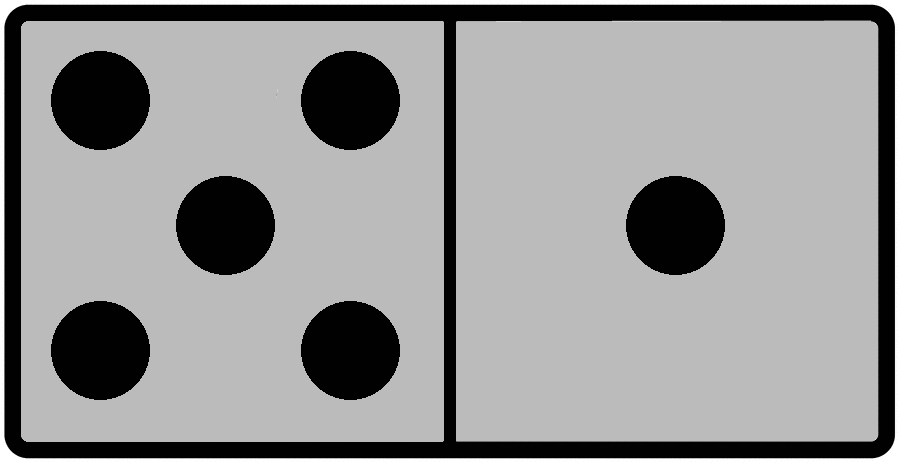
\includegraphics[width=0.3\textwidth]{gray5_1.png}
\hspace{.3in}
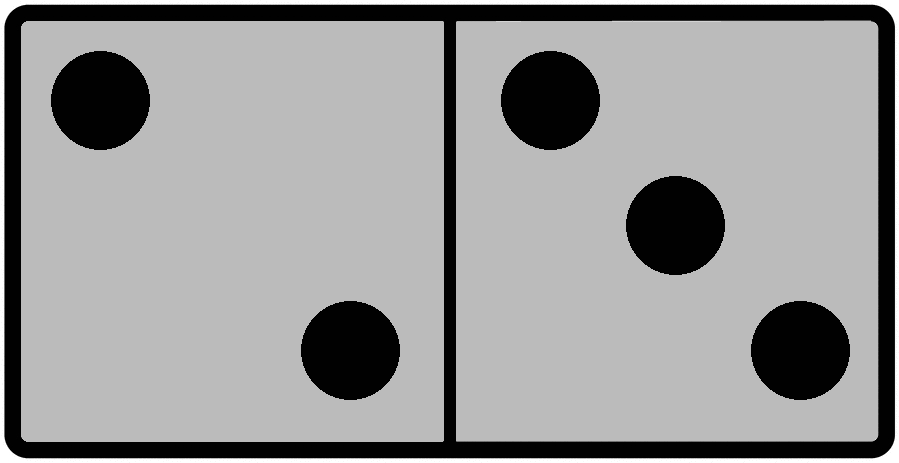
\includegraphics[width=0.3\textwidth]{gray2_3.png}
\end{center}

and your goal domino is:
\begin{center}
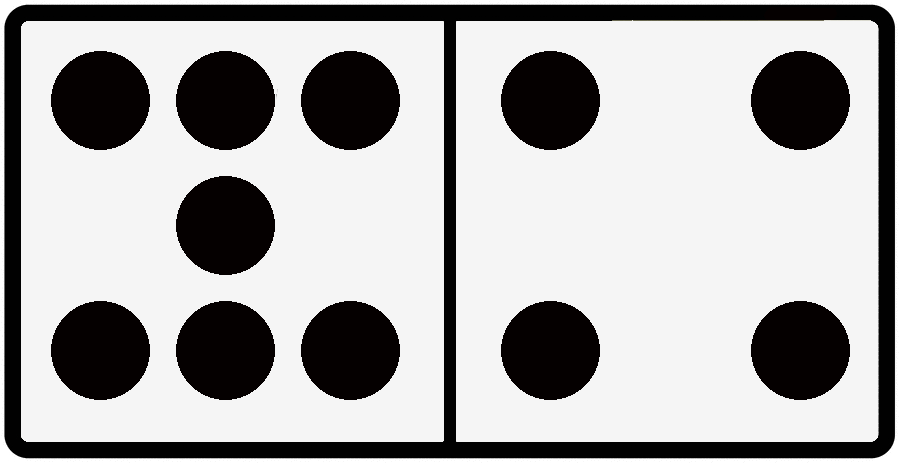
\includegraphics[width=0.3\textwidth]{white7_4.png}
\end{center}

A solution would be ``\textbf{one} and \textbf{one}.'' This means that you'll
take \textit{one} copy of the first starter domino, and \textit{one} copy of
the second, and add them together.

\begin{center}
{\LARGE Solution: \textbf{1 \& 1}}

1 \raisebox{-0.3\height}{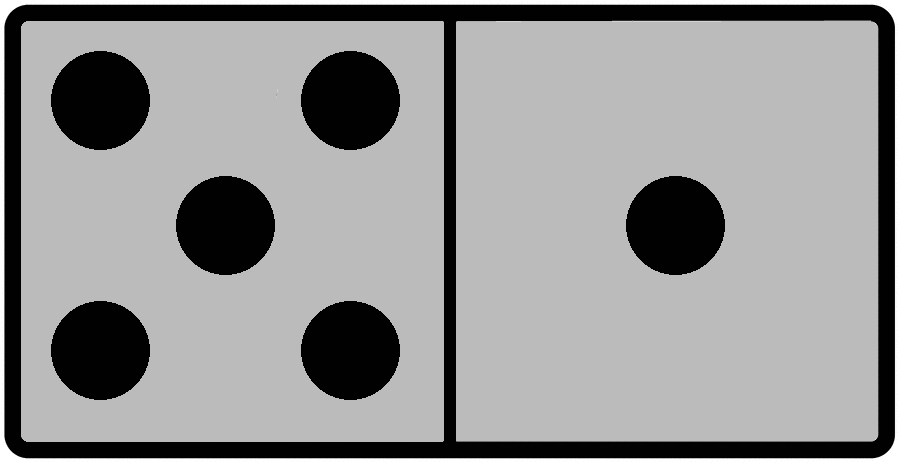
\includegraphics[width=0.1\textwidth]{gray5_1.png}} \ \& \
1 \raisebox{-0.3\height}{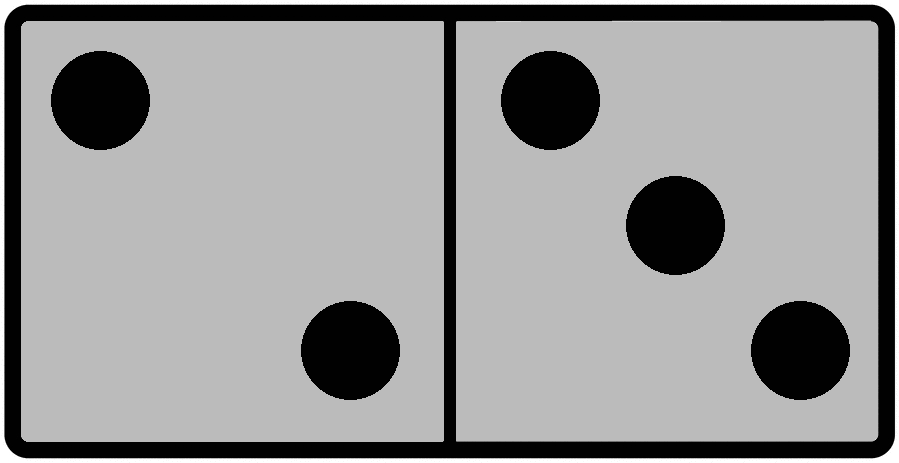
\includegraphics[width=0.1\textwidth]{gray2_3.png}} \ = \
\raisebox{-0.3\height}{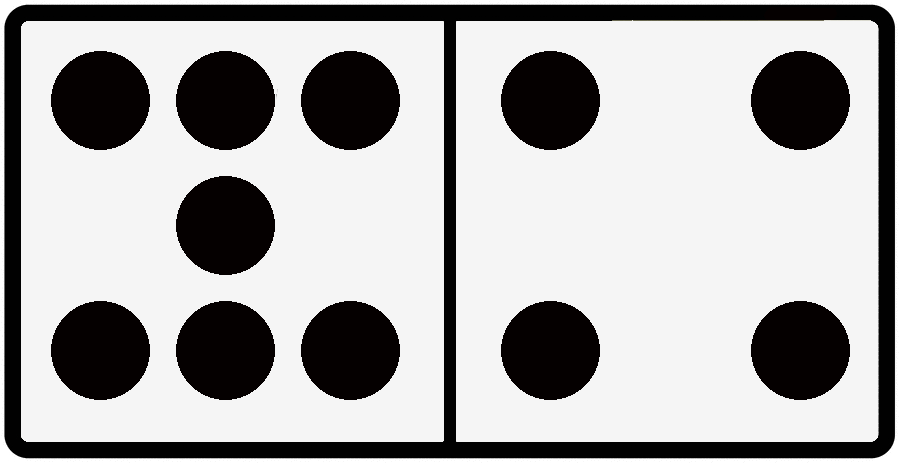
\includegraphics[width=0.1\textwidth]{white7_4.png}} \quad
\end{center}

Stare carefully at that until you master how it works; the rest of this chapter
will be a complete waste of time if this operation is not fully grasped. Adding
domino 5--1 to 2--3 means adding the left sides together, and separately adding
the right sides together, to produce a new domino 7--4 (since $5+2=7$ and
$1+3=4$).

\subsection{Actually do this}

All right, let's test your skillz. I want you to \textit{actually} work out the
answers to the following Domino Game puzzles on your own. There are six of
them, so it might take you a while (perhaps as long as 6 minutes). But it's
vital to cement your understanding of how this works...\textit{and} to set up
the crucial punchline later on in this chapter.

Answers to each puzzle are given at the end of the chapter. Maybe your answers
will not be the same as mine...or maybe they will? That itself is actually a
very important question we'll consider in a few minutes.

Enough preamble. Go!

\begin{enumerate}
\itemsep2em

\label{startDominoPuzzes}
\item Starter dominoes:
\hspace{.3in}
\raisebox{-0.3\height}{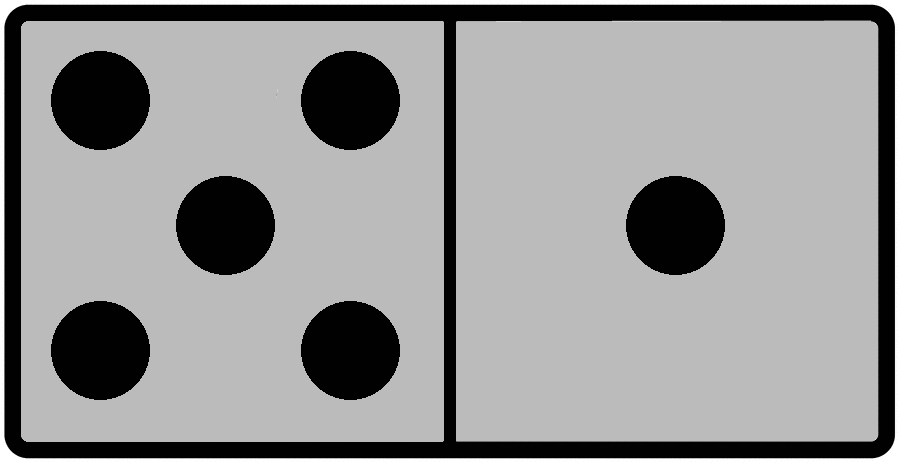
\includegraphics[width=0.2\textwidth]{gray5_1.png}}
\hspace{.1in}
\raisebox{-0.3\height}{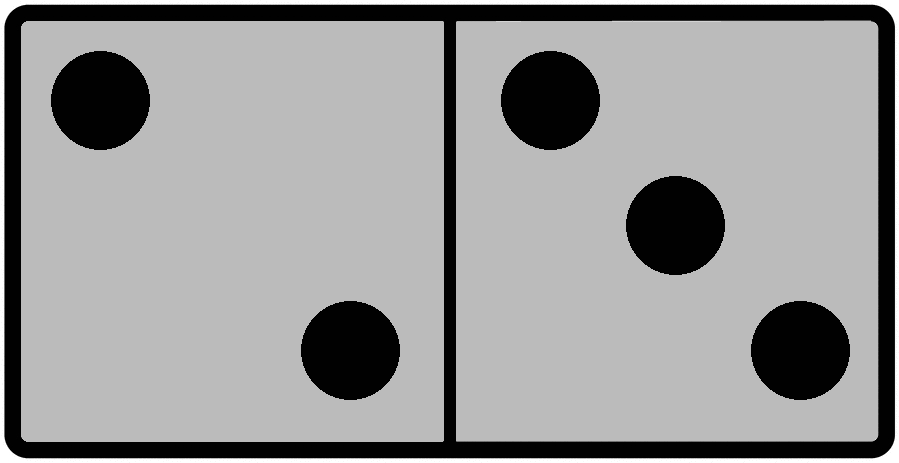
\includegraphics[width=0.2\textwidth]{gray2_3.png}}

Goal domino:
\hspace{1.1in}
\raisebox{-0.3\height}{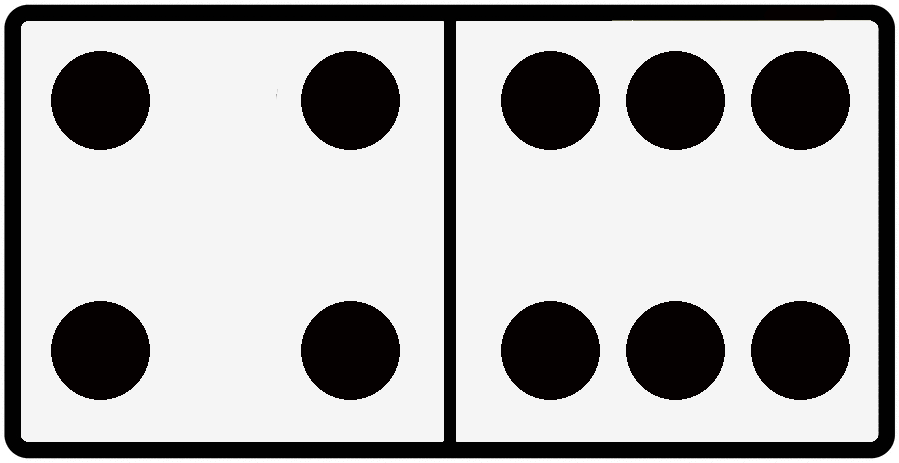
\includegraphics[width=0.2\textwidth]{white4_6.png}}

\footnotesize
(Hint: it's okay to take \textit{zero} of one of the dominoes; \textit{i.e.},
to completely ignore it.)
\normalsize

\item Starter dominoes:
\hspace{.3in}
\raisebox{-0.3\height}{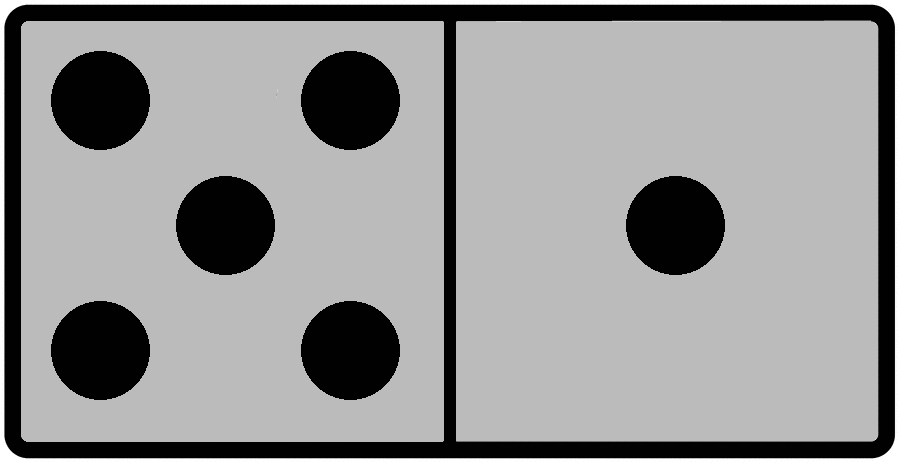
\includegraphics[width=0.2\textwidth]{gray5_1.png}}
\hspace{.1in}
\raisebox{-0.3\height}{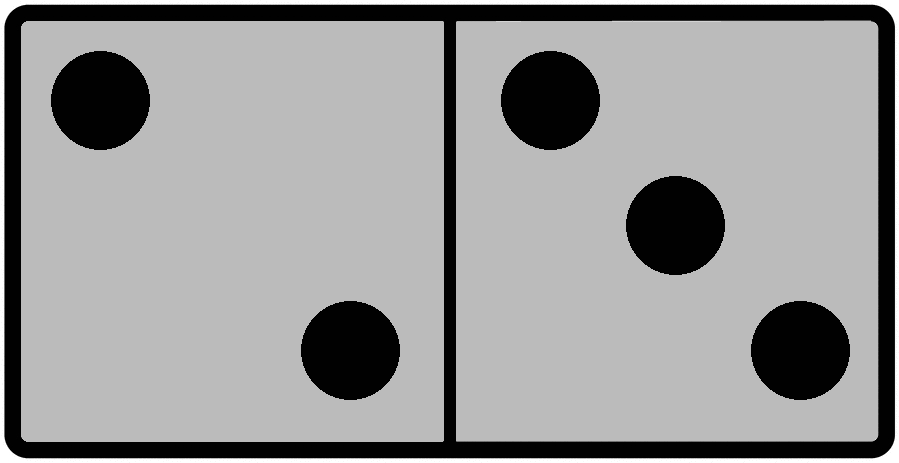
\includegraphics[width=0.2\textwidth]{gray2_3.png}}

Goal domino:
\hspace{1.1in}
\raisebox{-0.3\height}{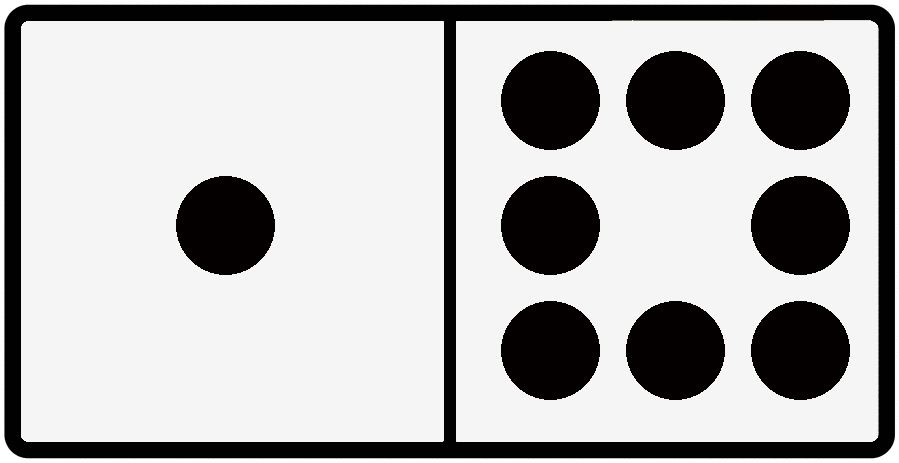
\includegraphics[width=0.2\textwidth]{white1_8.png}}

\footnotesize
(Hint: you may, if you wish, take ``a \textit{negative} number'' of one of the
dominoes. In other words, you can multiply the entire domino by a negative
number and then add it to your multiples of the other one.)
\normalsize

\item Starter dominoes:
\hspace{.3in}
\raisebox{-0.3\height}{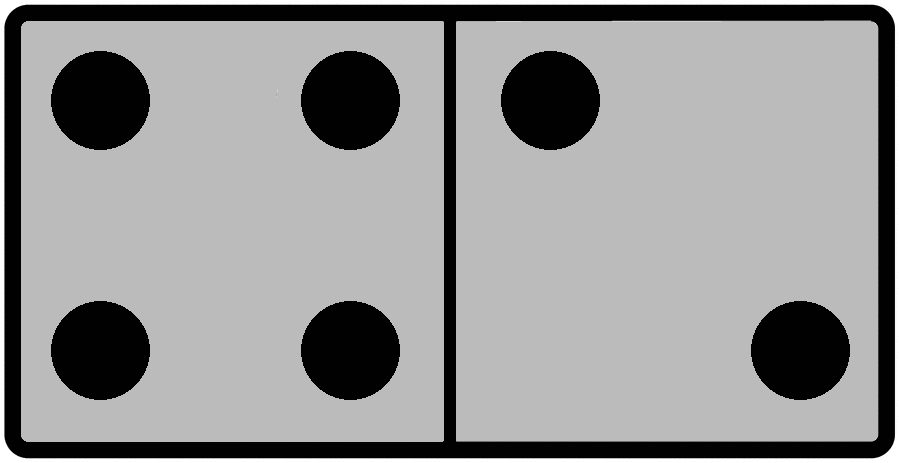
\includegraphics[width=0.2\textwidth]{gray4_2.png}}
\hspace{.1in}
\raisebox{-0.3\height}{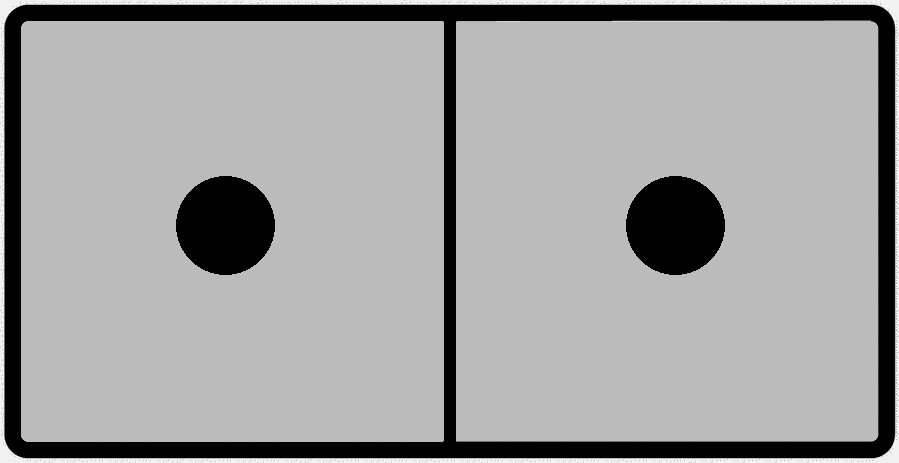
\includegraphics[width=0.2\textwidth]{gray1_1.png}}

Goal domino:
\hspace{1.1in}
\raisebox{-0.3\height}{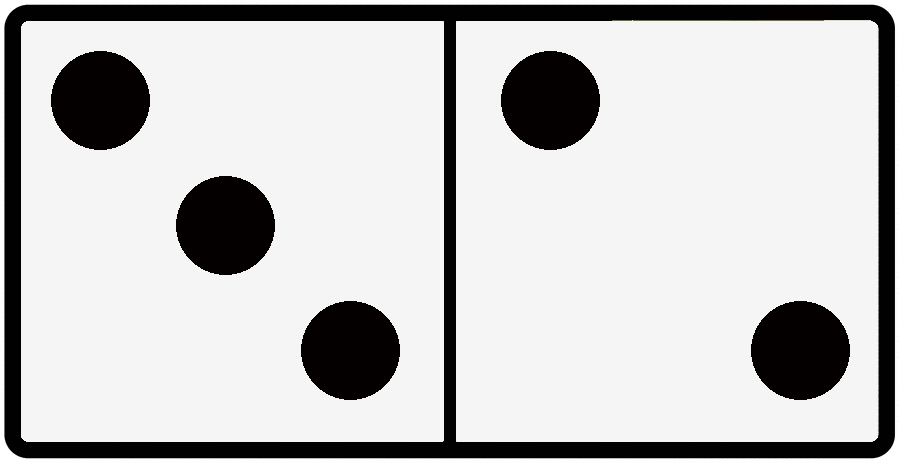
\includegraphics[width=0.2\textwidth]{white3_2.png}}

\footnotesize
(Hint: you can even take a \textit{fraction} of a domino, provided you take the
same fraction of both left and right sides. This means that just as you can
multiply an entire domino by a positive or negative number, or zero, you can
also multiply it by non-integers.)
\normalsize

\pagebreak
\item Starter dominoes:
\hspace{.3in}
\raisebox{-0.3\height}{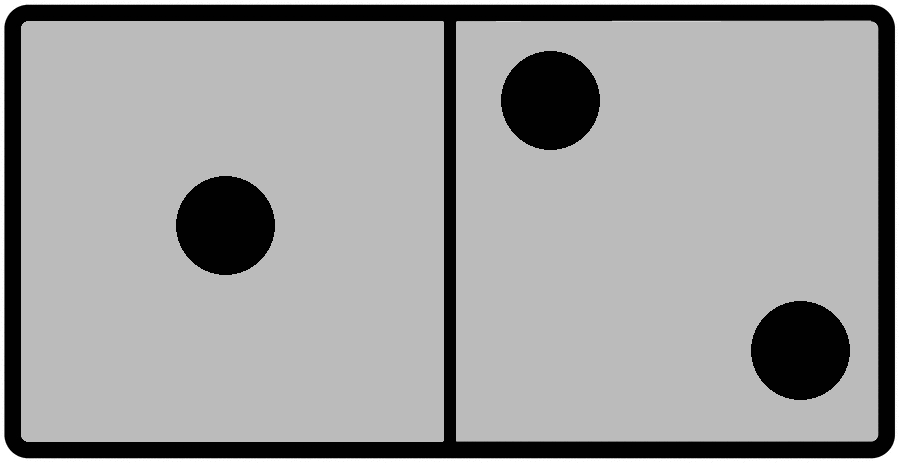
\includegraphics[width=0.2\textwidth]{gray1_2.png}}
\hspace{.1in}
\raisebox{-0.3\height}{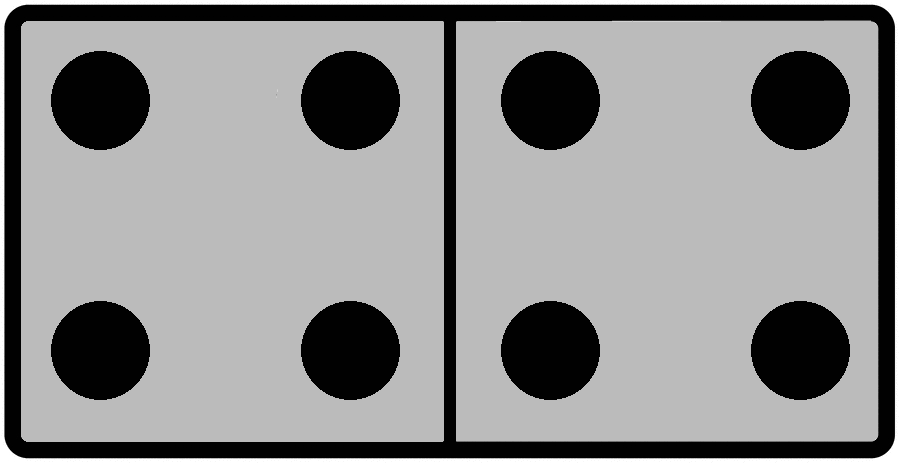
\includegraphics[width=0.2\textwidth]{gray4_4.png}}

Goal domino:
\hspace{1.1in}
\raisebox{-0.3\height}{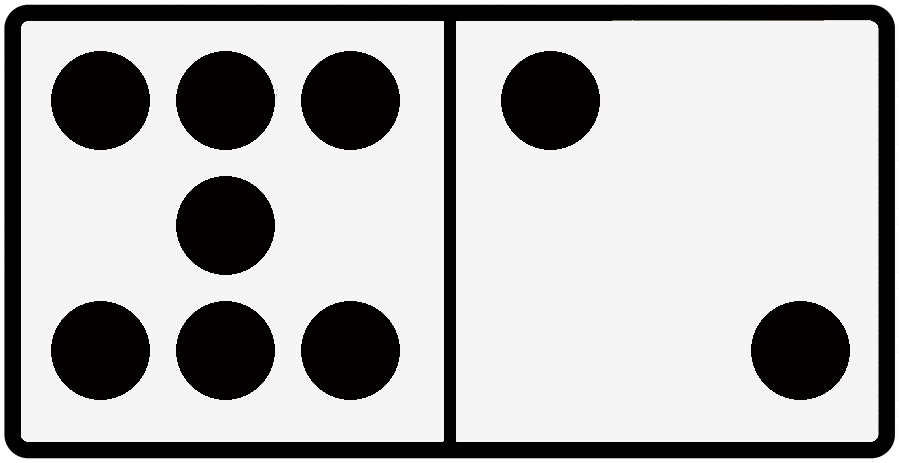
\includegraphics[width=0.2\textwidth]{white7_2.png}}

\footnotesize
(Hint: sometimes you have to go pretty far afield to get a solution, meaning a
large number of one domino and a large \textit{negative} number of the other.)
\normalsize

\item Starter dominoes:
\hspace{.3in}
\raisebox{-0.3\height}{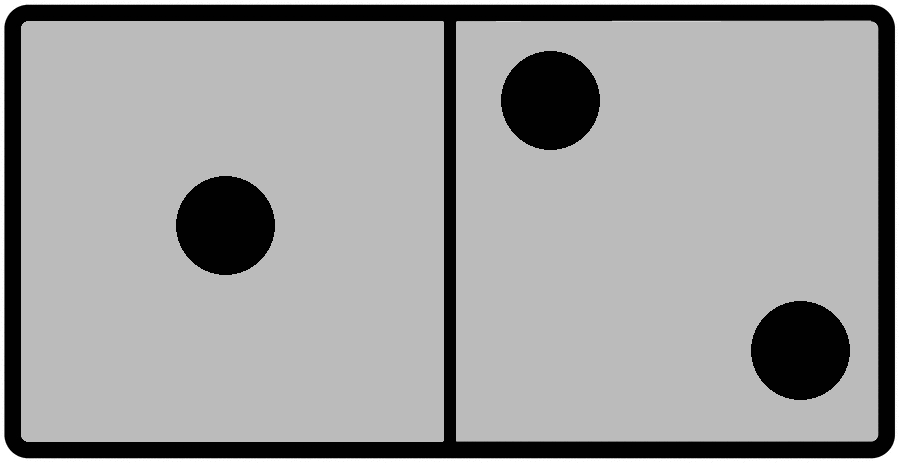
\includegraphics[width=0.2\textwidth]{gray1_2.png}}
\hspace{.1in}
\raisebox{-0.3\height}{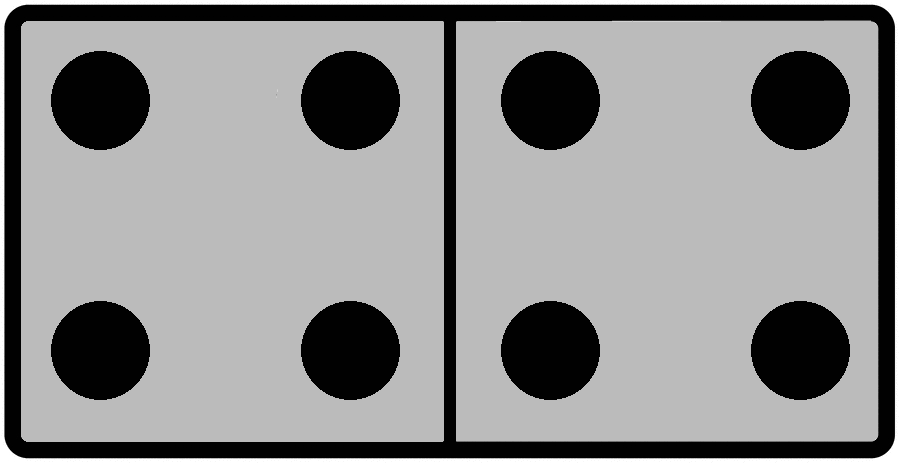
\includegraphics[width=0.2\textwidth]{gray4_4.png}}

Goal domino:
\hspace{1.1in}
\raisebox{-0.3\height}{
\includegraphics[width=0.2\textwidth]{white0_4.png}}

\footnotesize
(Hint: the goal domino can have a zero on it, just like the starter dominoes
did. But it's really no different; you just have to think creatively about how
to get the numbers to add up to zero on that side.)
\normalsize

\item Starter dominoes:
\hspace{.3in}
\raisebox{-0.3\height}{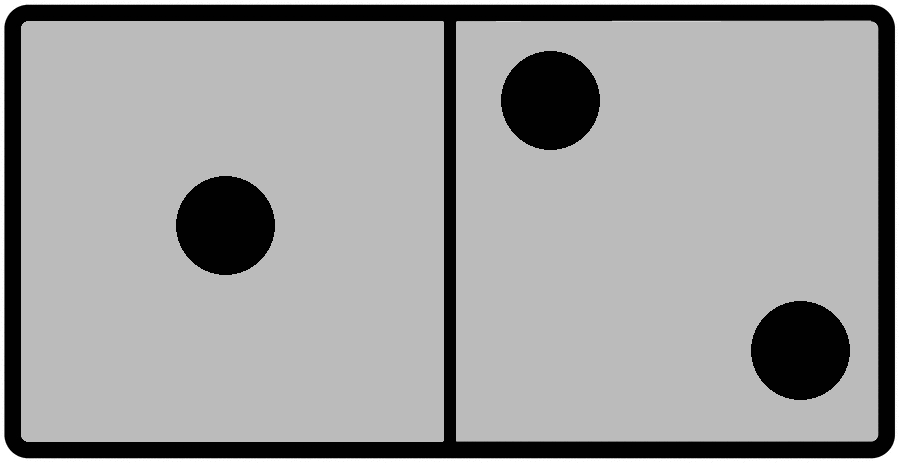
\includegraphics[width=0.2\textwidth]{gray1_2.png}}
\hspace{.1in}
\raisebox{-0.3\height}{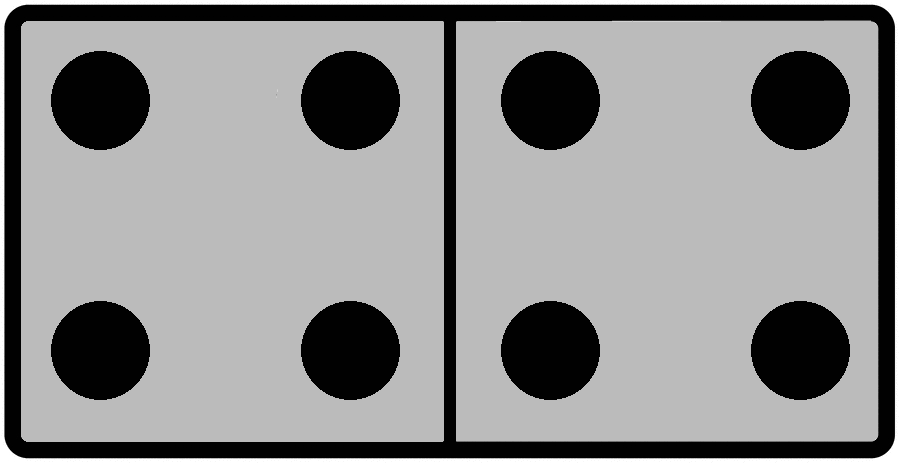
\includegraphics[width=0.2\textwidth]{gray4_4.png}}

Goal domino:
\hspace{1.1in}
\raisebox{-0.3\height}{
\includegraphics[width=0.2\textwidth]{white0_0.png}}

\footnotesize
(Hint: and yeah, the goal domino might even be \textit{completely} zero. That's
really not any different either, and in fact the solution will probably just
jump right off the page at you.)
\normalsize
\label{endDominoPuzzes}
\end{enumerate}

\subsection{Questions for curious minds}

I presume you have tried it, and hopefully succeeded at a few by trial and
error. Even if you didn't, hopefully you looked at and understood the solutions
I gave at the end of the chapter (p.~\pageref{dominoPuzzleAnswers}).

It's well worth taking a moment after all that fiddling around to consider some
interesting questions:

\begin{enumerate}
\itemsep.1em

\item Were your solutions that same as mine in each case? If so, do you think
that was just coincidence? If not, how many different solutions do you think
are possible?

\item Is it always possible to solve a puzzle like this, no matter what the
goal domino is? Or are only a small number of goal dominoes actually possible
to produce?

\item Is it always possible to solve a puzzle like this, no matter what the
starter dominoes are? Or is it only in a few cleverly crafted scenarios where
the numbers happen to work out just right?

\end{enumerate}

We'll shed light on all these matters as we move forward.

\pagebreak
\subsection*{Answers to Domino Game puzzles from
pp.~\pageref{startDominoPuzzes}-\pageref{endDominoPuzzes}}
\label{dominoPuzzleAnswers}

\begin{enumerate}
\itemsep1em

\item {Solution: \textbf{0 \& 2}}

\quad 0 \raisebox{-0.3\height}{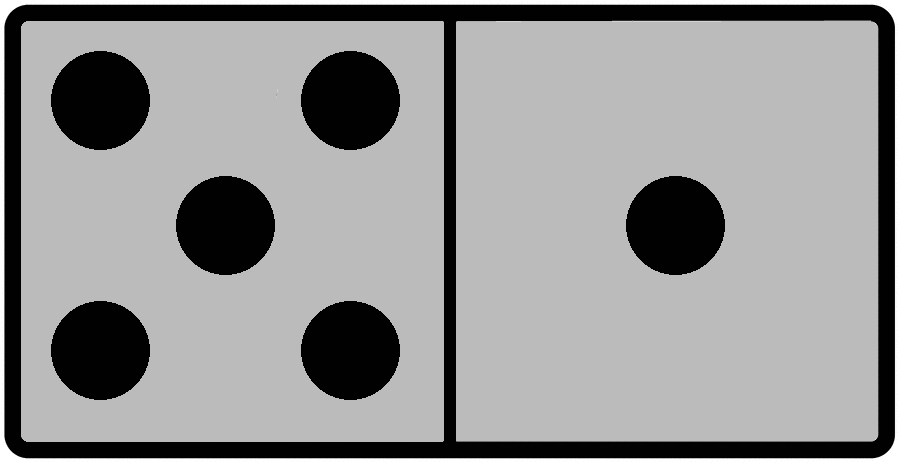
\includegraphics[width=0.1\textwidth]{gray5_1.png}} \ \& \
2 \raisebox{-0.3\height}{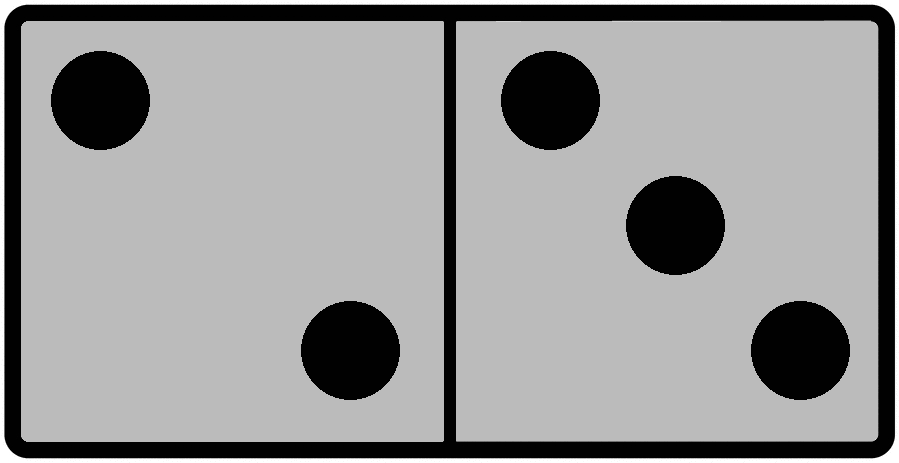
\includegraphics[width=0.1\textwidth]{gray2_3.png}} \ = \
\raisebox{-0.3\height}{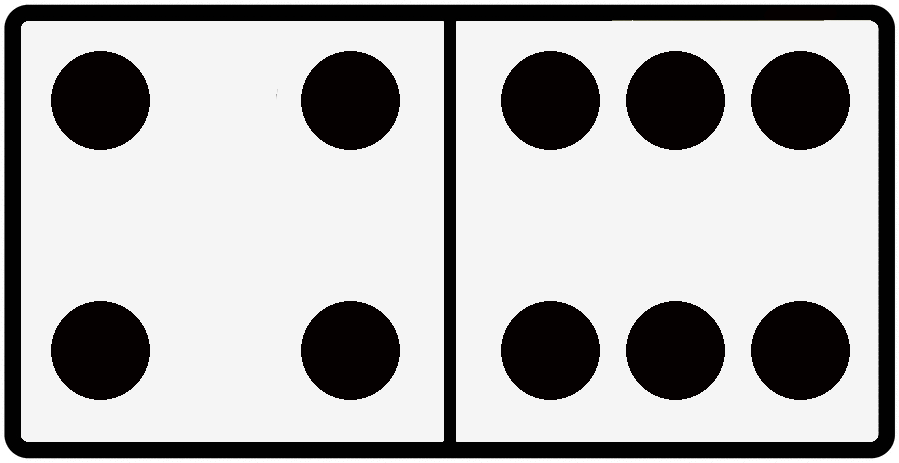
\includegraphics[width=0.1\textwidth]{white4_6.png}} \quad

\item {Solution: \textbf{--1 \& 3}}

\ $-1$ \raisebox{-0.3\height}{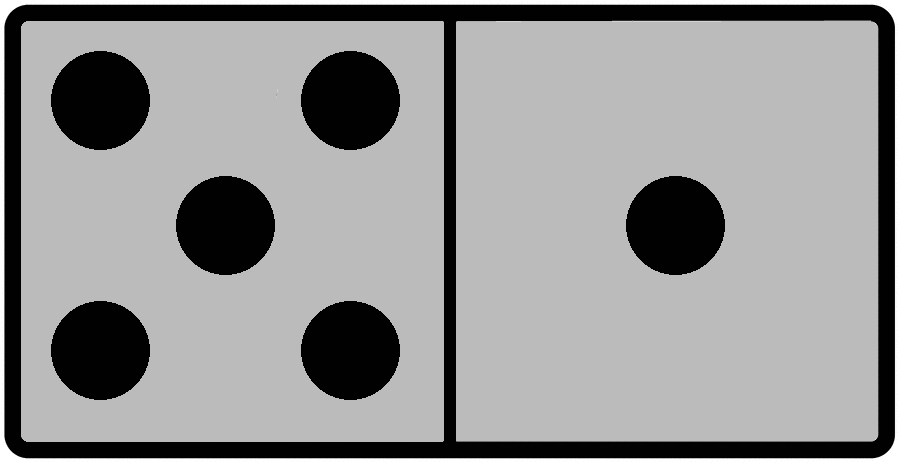
\includegraphics[width=0.1\textwidth]{gray5_1.png}} \ \& \
3 \raisebox{-0.3\height}{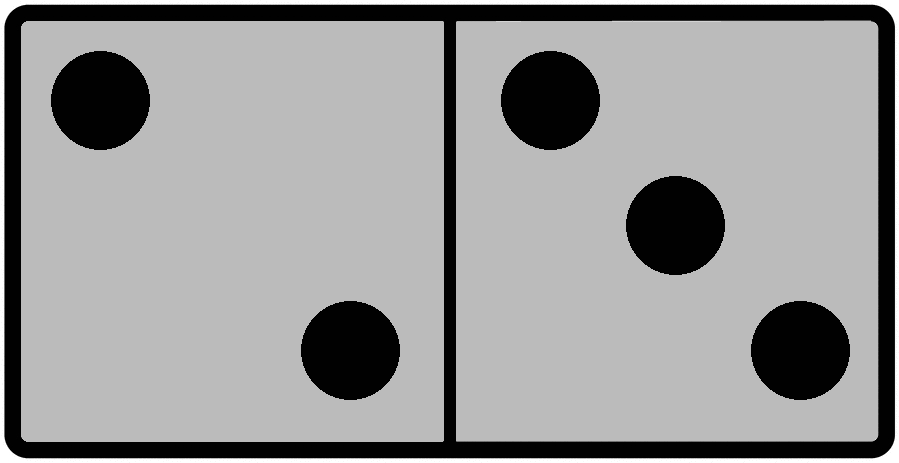
\includegraphics[width=0.1\textwidth]{gray2_3.png}} \ = \
\raisebox{-0.3\height}{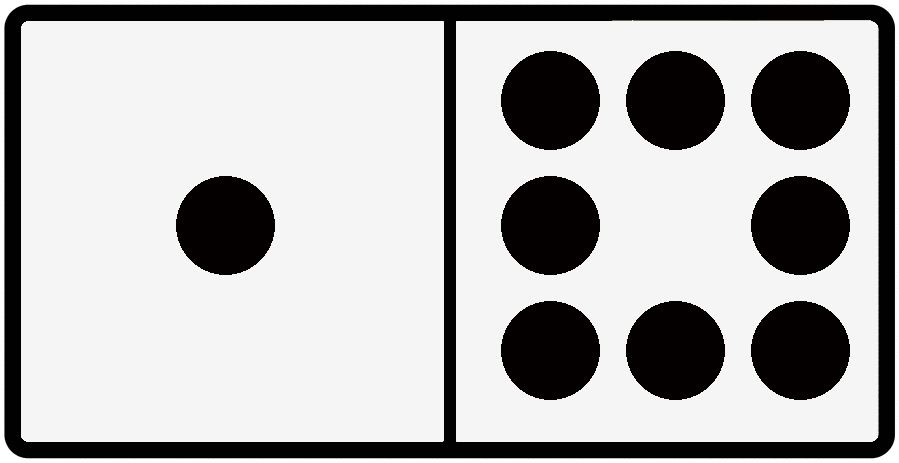
\includegraphics[width=0.1\textwidth]{white1_8.png}} \quad

\item {Solution: \textbf{$\frac{1}{2}$ \& 1}}

\quad $\frac{1}{2}$ \raisebox{-0.3\height}{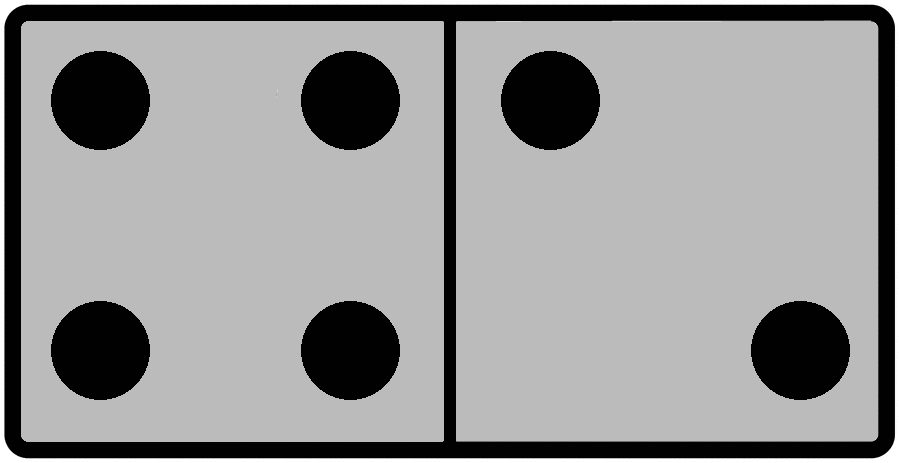
\includegraphics[width=0.1\textwidth]{gray4_2.png}} \ \& \
1 \raisebox{-0.3\height}{\includegraphics[width=0.1\textwidth]{gray1_1.png}} \ = \
\raisebox{-0.3\height}{\includegraphics[width=0.1\textwidth]{white3_2.png}} \quad

\item {Solution: \textbf{-5 \& 3}}

\ $-5$ \raisebox{-0.3\height}{\includegraphics[width=0.1\textwidth]{gray1_2.png}} \ \& \
3 \raisebox{-0.3\height}{\includegraphics[width=0.1\textwidth]{gray4_4.png}} \ = \
\raisebox{-0.3\height}{\includegraphics[width=0.1\textwidth]{white7_2.png}} \quad

\item {Solution: \textbf{4 \& --1}}

\quad 4 \raisebox{-0.3\height}{\includegraphics[width=0.1\textwidth]{gray1_2.png}} \&
$-1$ \raisebox{-0.3\height}{\includegraphics[width=0.1\textwidth]{gray4_4.png}} \ = \
\raisebox{-0.3\height}{\includegraphics[width=0.1\textwidth]{white0_4.png}} \quad

\item {Solution: \textbf{0 \& 0}}

\quad 0 \raisebox{-0.3\height}{\includegraphics[width=0.1\textwidth]{gray1_2.png}} \ \& \
0 \ \raisebox{-0.3\height}{\includegraphics[width=0.1\textwidth]{gray4_4.png}} \ = \
\raisebox{-0.3\height}{\includegraphics[width=0.1\textwidth]{white0_0.png}} \quad

\end{enumerate}


\chapter{Matrices}

It's now time for the granddaddy of all linear algebra entities: the
\textbf{matrix}. When we've finished this part of our climb, you'll actually be
able to see the summit we'll eventually reach.

By the way, the plural of \textit{matrix} is \textbf{matrices} (pronounced
MAY-trih-sees), kind of like the plural of \textit{index} is \textit{indices.}
But don't forget the singular is still ``\textit{matrix}!'' Don't let me (or
anyone else) catch you uttering the non-word ``matrice'' -- you'll sound like a
dweeb and drive me up a wall.

\section{Row and column vectors}
\index{vector}

Up to now, a vector has simply been a vector. I haven't made a big deal about
how you write it on the page. We've been free to write a vector
$\overrightarrow{\textbf{x}}$ with the three elements 6, 2, and 9 in either of
these ways:

\vspace{-.15in}
\begin{center}
\begin{tabular}{ccc}
$\overrightarrow{\textbf{x}}$ = \textbf{[}$\ 6\ \ 2\ \ 9\ $\textbf{]} &
\quad\quad \textit{...or...} \quad\quad &
$\overrightarrow{\textbf{x}}$ = $\begin{bmatrix} 6 \\ 2 \\ 9 \end{bmatrix}$ \ 
\end{tabular}
\end{center}
\vspace{-.15in}

\index{function}

Or heck, you could even write it diagonally if you want. This flexibility is
because all that really matters is the \textit{function} view of a vector that
we discussed in section~\ref{vectorIsFunction}. All that ultimately matters is
that you associate the correct index number with the correct element. However I
might draw $\overrightarrow{\textbf{x}}$ on paper, if I asked you for the value
of ``element \#0,'' you'd say 6, and if I asked for ``element \#2,'' you'd say
9. The way it looks has been immaterial up until now.

\index{row vector}
\index{column vector}

That will still be true sometimes. But beginning with this chapter, it's going
to sometimes turn out to matter whether or not we think of a vector as a
\textbf{row vector} (the left-hand-side version of
$\overrightarrow{\textbf{x}}$, above) or a \textbf{column vector} (the
right-hand-side). Memorize these terms: they matter, and you'll have to have
them on the tip of your neural cortex. A row goes horizontally, side-to-side;
and a column goes vertically, up-to-down.

I'll try to always be very careful to emphasize the row vs.~column nature of a
vector in those cases where it turns out to matter.

\index{default}

By the way, one surprising thing (at least, it was to me) is that the
``default'' is for an unspecified vector to be treated as a \textit{column}
vector, not a row. Column vectors take up more room on the page, and aren't as
natural when you're writing on paper, which I guess is why it surprised me. At
any rate, whenever a vector is under discussion, try to visualize it as an
up-and-down column of entries, unless the accompanying text explicitly says
otherwise.

\section{The matrix}

\index{matrix (plural: matrices)}

At last, the matrix. This will seem underwhelming at first, but \textit{boy}
does it pack a wallop.

A matrix is simply a two-dimensional rectangular grid of entries, kind of like
a spreadsheet. We'll use capital letters to designate them, with no special
arrow-like or other adornment. Here's our first example:

\vspace{-.15in}
\begin{align*}
A =
\begin{bmatrix}
5 &-7 &3 &9 \\
18 &4 &1 &1 \\
3 &-3 &\pi &4 \\
\end{bmatrix}
\end{align*}
\vspace{-.15in}

\index{dimension}

Matrices are always rectangular, but not always square. The $A$ matrix is
called a ``$3\times 4$'' (three-by-four) matrix, since it has three
\textbf{row}s and four \textbf{column}s. We say that $3\times 4$ are the
matrix's \textbf{dimensions}. Again, it's important to master all this
terminology. When giving the dimensions of a matrix, you always list the number
of rows first, and then the number of columns.

\index{index number}

To specify an individual element, we need \textit{two} indices instead of just
one as we did for a vector. We'll use Python-style numbering (starting with 0)
and write the row and column as a two-part comma-separated subscript:

\vspace{-.15in}
\begin{align*}
A_{0,0} &= 5 \\
A_{1,0} &= 18 \\
A_{0,3} &= 9 \\
A_{2,2} &= \pi \\
\end{align*}
\vspace{-.25in}

Just practice first moving down to the correct row, then moving over to the
correct column, and you'll be fine.

\subsection{Labels}

\index{label}

As with vectors, we won't always use index numbers to designate rows and
columns: sometimes we'll use labels. Check out this matrix $W$ (for
``weather''):

\vspace{-.4in} 
\begin{adjustwidth}{}{60pt}
\begin{center}
\begin{multicols}{2}
\begin{flushright}
\hspace*{1cm} \\
\hspace*{1cm} \\
\footnotesize{D.C.} \\
\footnotesize{Fredericksburg} \\
\footnotesize{Richmond} \\
\end{flushright}
\columnbreak
\vspace{-1.5in} 
\begin{align*}
\begin{bmatrix}
81 \ & \ 86 \ & \ 78 \ & \ 74 \ & \ 77 \\
83 \ & \ 86 \ & \ 79 \ & \ 79 \ & \ 82 \\
82 \ & \ 86 \ & \ 84 \ & \ 87 \ & \ 87 \\
\end{bmatrix}
\end{align*}
\vspace{-.15in}
\scriptsize{Mon} \ \  \scriptsize{Tue} \ \ \scriptsize{Wed} \ \ \scriptsize{Thu} \ \ \scriptsize{Fri} \\
\end{multicols}
\end{center}
\end{adjustwidth}
\vspace{-.15in}

Here we're using city names for the row labels, and days of the week as the
column labels. It's still easy peasy to interpret -- how hot did it get in the
nation's capital on Tuesday? 86\textdegree, of course. Using the same subscript
notation as above, we could say:

\vspace{-.15in}
\begin{align*}
W_{\textrm{D.C.},\textrm{Mon}} &= 81 \\
W_{\textrm{Fredericksburg},\textrm{Wed}} &= 79 \\
W_{\textrm{Fredericksburg},\textrm{Thu}} &= 79 \\
W_{\textrm{Richmond},\textrm{Thu}} &= 87 \\
&\vdots \\
\end{align*}

and so forth. D.C. and Fred had a bit of a cool-down midweek, thank God, while
Richmond was all the while cooking in the upper 80's.

\section{A matrix is also a function}

\index{function}
Remember back in section~\ref{vectorIsFunction} (p.~\pageref{vectorIsFunction})
when I explained that a vector, viewed in a sufficiently weird way, was
actually a function? The same thing is true for matrices, just by adding one
more input to the function.

Put another way, let's consider the row labels (or numbers, if we want to be
boring) as the set $C$ (for ``cities''). And let's consider the column labels
as the set $D$ (for ``days-of-the-week''). Then, you can see that a matrix is
precisely maps a pair of a city and a day to a high temperature. (The high
temperatures are in the set $\mathbb{R}$, which are the real numbers.) In
symbols, $W$ is defined as this function:

\vspace{-.15in}
\begin{align*}
W : C \times D \rightarrow \mathbb{R}
\end{align*}
\vspace{-.15in}

\index{domain}
\index{codomain}
\index{Cartesian product}
Recall that function syntax. $W$ is the name of the function. The part before
the arrow is the \textbf{domain} of the function: the set which its inputs are
drawn from. Since it's the Cartesian product of two sets (cities and days) this
domain is really all the ordered pairs of cities-and-days, like (D.C., Thurs)
and (Richmond, Monday). The function takes any ordered pair like that and gives
you a number telling you how hot that city was on that day. It's a snap when
seen this way.


\section{Matrix operations}

Just as section~\ref{vectorOps} listed the permissible actions we could perform
on vectors (and scalars), so this section lists the operations we can perform
on matrices (and vectors, and scalars). There's one other big one which I'll
save for entire separate chapter, but there are still four useful ones we'll
cover here.

\subsection{Operation \#1: scalar-matrix multiplication}

This one's a piece of cake. Recall that multiplying a scalar by a vector
amounted to multiplying the scalar by each of its elements, producing a vector
of the same dimension. Same here: we get a matrix of the same dimension by
multiplying individually:

\vspace{-.15in}
\begin{align*}
4 \cdot
\begin{bmatrix}
3 & 2 & 9 \\
1 & -1 & 0 \\
\end{bmatrix}
=
\begin{bmatrix}
12 & 8 & 36 \\
4 & -4 & 0 \\
\end{bmatrix}.
\end{align*}
\vspace{-.15in}

Sometimes we'll put a dot between the two, as above, though we'll often omit
that and just write the scalar and matrix side-by-side. Either way, it means
scalar-matrix multiplication.

\subsection{Operation \#2: matrix addition}

Also a piece of cake, and just what you'd expect:

\vspace{-.15in}
\begin{align*}
\begin{bmatrix}
4 & 1 \\
1 & -2 \\
3 & 18 \\
\end{bmatrix}
\begin{bmatrix}
1 & 2 \\
5 & 2 \\
-10 & -10 \\
\end{bmatrix}
+
\begin{bmatrix}
5 & 3 \\
6 & 0 \\
-7 & 8 \\
\end{bmatrix}.
\end{align*}
\vspace{-.15in}

The only hard part is not going cross-eyed as you zigzag your eyeballs across
the page to match up entries.

As with vector addition, you simply can't add two matrices at all if they don't
have the same dimensions. Also just like vectors, we can \textit{subtract} one
matrix from another just by adding the first matrix to ``$-1$ times the second
matrix.''

%transpose
%2x3 transpose gives us 3x2.  (Ai,j = ATj,i)
%
%use transpose on a row vector to get a column vector.
%(Treating the vector as a one-row / one-col matrix when we do this)
%
%
%matrix-vector multiplication. not what you'd expect. not even the kind of
%result you'd expect.
%
%Make A a 4x2, x a column vector 2x1.
%if mxn matrix, you need a n-dimensional column vector (or "nx1 matrix")
%weird! # of rows of one must be # of columns of the other.
%get an mx1 answer!
%
%two different ways to think about this A dot xvector.
%
%1. All the dot products of the vector with the matrix's rows.
%2. A linear combination of the matrix's columns (with the vector's elements as
%coefficients.)
%
%Show the second thing all worked out as the linear combo of columns.
%
%
%Why think about it as way 1? Jezebel col vector, matrix of all the guys (heck,
%let's put guys surveys in columns too, then that requires transpose
%
%
%Why think about it in way 2? Recipes matrix. each column is one recipe, each
%row is an ingredient. Vector shows how many of each recipe you want to make.
%


\chapter{Linear transformations}

\index{linear transformation}
\index{function}

A \textbf{linear transformation} is actually just another spin on matrix-vector
multiplication. It's also yet another way to view a matrix as a
\textit{function}. Back on p.~\pageref{matrixIsFunction}, I made the point that
instead of drawing numbers in a grid, you could view a matrix itself as a
function, where the input is an ordered pair (row and column numbers) and the
output is the element at that entry. In this chapter, we explore a deeper and
richer interpretation of a matrix as a \textit{different} sort of function.

\section{Transforming one vector into another}

Recall how matrix-vector multiplication works. We'll write it notationally as
$A \cdot \overrightarrow{\textbf{x}} = \overrightarrow{\textbf{y}}$, where
$\overrightarrow{\textbf{y}}$ is the result of the multiplication. Now we could
think about the operation like this:

\begin{compactitem}
\item $A$ is a ``function'' of sorts, which works on vectors to produce other
vectors.
\item $\overrightarrow{\textbf{x}}$ is the input vector we give to that
function.
\item $\overrightarrow{\textbf{y}}$ is the function's output (result).
\end{compactitem}

\index{machine}
We're thinking of $A$ as a long-lasting, reusable thing, whereas
$\overrightarrow{\textbf{x}}$ and $\overrightarrow{\textbf{y}}$ stand for the
temporary inputs \& outputs that we give to $A$ and compute on the fly. My
mental image is of $A$ as a machine, $\overrightarrow{\textbf{x}}$ as the raw
materials we might feed to the machine, and $\overrightarrow{\textbf{y}}$ as
the machine's completed work.

One natural question is: ``what is the domain, and the range, of this $A$
function?'' That depends on $A$'s dimensions. Suppose it's a $3\times 2$
matrix:

\vspace{-.15in}
\begin{align*}
\begin{bmatrix}
2 & 3 \\
1 & -4 \\
0 & 5 \\
\end{bmatrix} \cdot \textrm{\Large ?} = \textrm{\Large ?}
\end{align*}
\vspace{-.15in}

\index{domain}
\index{codomain}
We know from the rules of matrix-vector multiplication
(p.~\pageref{matVecRules}) that the first question mark has to be a
\textbf{2}-dimensional column vector, else the operation is impossible. And we
know that the output will be a \textbf{3}-dimensional column vector. This means
that the domain of the $A$ ``function'' is 2-d vectors and the codomain is 3-d
vectors. Most commonly, this is written as follows:

\vspace{-.15in}
\begin{align*}
A : \mathbb{R}^2 \rightarrow \mathbb{R}^3.
\end{align*}
\vspace{-.15in}

Remember from \textit{A Cool, Brisk Walk} that the $\mathbb{R}$ sign means
``the set of real numbers.'' When we say ``$\mathbb{R}^2$'' we're saying ``the
set of vectors with two real-numbered entries.'' And $\mathbb{R}^3$ is the set
of \textit{three}-dimensional real vectors, \textit{etc.}

Put all together, the purpose of our $A$ matrix is to map each two-dimensional
vector to a particular three-dimensional vector. For instance, it maps the 2-d
vector $[\ 2 \ \ 1\ ]$ to:

\vspace{-.15in}
\begin{align*}
\begin{bmatrix}
2 & 3 \\
1 & -4 \\
0 & 5 \\
\end{bmatrix} \cdot 
\begin{bmatrix}
2 \\ 1 \\
\end{bmatrix} =
\begin{bmatrix}
7 \\ -2 \\ 5 \\
\end{bmatrix}.
\end{align*}
\vspace{-.15in}

The particular vector it chooses seems kind of random so far, and indeed this
first example is just pulled from the air. Normally there will be some
``meaning'' to the transformation.

\index{linear map}

By the way, a linear transformation is sometimes called a \textbf{linear map}
because it performs this ``mapping'' operation, like a function does. The two
terms (linear transformation and linear map) are exact synonyms.

\subsection{Meaningful examples}

Before we go any further, let's at least show that this is useful. I'm going to
create a machine (matrix) $B$ (for ``Body,'' sort of) that transforms certain
4-dimensional vectors into 2-dimensional ones. Here it is:

\vspace{-.15in}
\begin{align*}
B = 
\begin{bmatrix}
12 & 1 & 0 & 0 \\
0 & 0 & 2.2 & 0 \\
\end{bmatrix}.
\end{align*}
\vspace{-.15in}

The kind of input this matrix/function is intended to act on a vector such as
$\overrightarrow{\textbf{stephen}}$, which is structured like this:

\vspace{-.3in} 
\begin{align*}
\begin{matrix*}[r]
\textrm{\small{height: whole feet}} \rightarrow \\
\textrm{\small{height: extra inches}} \rightarrow \\
\textrm{\small{weight: kilograms}} \rightarrow \\
\textrm{\small{shoe size}} \rightarrow \\
\end{matrix*}
\begin{bmatrix}
6 \\ 2 \\ 95.5 \\ 13 \\
\end{bmatrix}
\end{align*}
\vspace{-.15in}

This rather revealing vector contains some of my vital bodily stats. I'm 6'2"
tall, and hence don't fit on airplanes; I weigh too much at 95.5 kg; and I wear
an impossible-to-fit 13 shoe (13AAA, actually; blame my mom's side of the
family).

Now what happens when we feed this to the $B$ machine?

\vspace{-.15in}
\begin{align*}
B \cdot \overrightarrow{\textbf{stephen}} =
\begin{bmatrix}
12 & 1 & 0 & 0 \\
0 & 0 & 2.2 & 0 \\
\end{bmatrix} \cdot
\begin{bmatrix}
6 \\ 2 \\ 95.5 \\ 13 \\
\end{bmatrix} =
\begin{bmatrix}
74 \\ 210 \\
\end{bmatrix}
\begin{matrix*}[l]
\leftarrow \textrm{\small{height in inches}} \\
\leftarrow \textrm{\small{weight in pounds}} \\
\end{matrix*}
\end{align*}
\vspace{-.15in}

This matrix-vector multiplication produces a 2-element vector, since

\vspace{-.15in}
\begin{align*}
B : \mathbb{R}^4 \rightarrow \mathbb{R}^2.
\end{align*}
\vspace{-.15in}

The first element is my height in total inches, and the second element is my
weight in pounds. And it will do so for every person whose 4-dimensional vector
it's multiplied by. Interestingly, the shoe size of the input vector plays no
role in the value of the output vector, because there are zero elements at both
$B_{0,3}$ and $B_{1,3}$. And that's okay.

\smallskip
\index{BMI (body-mass index)}

By the way, you might think about expanding this example to calculate something
more complex like a BMI (body-mass index). After all, BMI is a straightforward
function of a person's weight and height, as you might know:

\vspace{-.15in}
\begin{align*}
\textrm{BMI} = 703 \times \frac{\textrm{weights (lbs)}}{\textrm{height (in)}^2}.
\end{align*}
\vspace{-.15in}

(Mine's about 27, which puts me in the obese range I'm sorry to inform you.)

However, it turns out this is \textit{impossible} to do with a linear
transformation. The reason is it's not linear! The only operations that can be
included in a linear transformation are dot products, because that's what
matrix-vector multiplication \textit{is}. So for each element of our output
vector, we can (1) take the elements of the input vector, (2) multiply each of
them by any constant we like, and (3) add up the results. The BMI formula, by
contrast, requires us to \textit{divide} one of our inputs by another, and in
fact requires us to \textit{square} that second input before dividing. These
are both decidedly non-linear operations that cannot be expressed with a
matrix.

This may seem limiting, and in a way it is, but keep in mind two things. First,
there are lots and lots and lots of common operations that \textit{are} linear,
and all of those come under our power in this book on linear algebra. Second,
when we do have linear operations, we can take advantage of all kinds of
computational simplifications and analytical tricks, so concentrating on the
linear case is most definitely worth our time.

\bigskip

Here's a second example. Suppose I have the following odd-looking matrix $S$
(for ``stocks,'' sort of):

\vspace{-.15in}
\begin{align*}
S =
\begin{bmatrix}
0 & 1 & 0 \\
0 & .69 & 0 \\
0 & 111.1 & 0 \\
0 & .88 & 0 \\
0 & 6.48 & 0 \\
0 & 17.37 & 0 \\
\end{bmatrix}
\end{align*}
\vspace{-.15in}

What does it do? Well, it's designed for us to feed it vectors representing
Wall Street stocks, like so:

\vspace{-.3in} 
\begin{align*}
\overrightarrow{\textbf{mcdonalds}} =
\begin{bmatrix}
1965 \\ 183.52 \\ 2606707 \\
\end{bmatrix}
\begin{matrix*}[l]
\leftarrow\textrm{\small{year founded}} \\
\leftarrow\textrm{\small{current share price}} \\
\leftarrow\textrm{\small{trading volume}} \\
\end{matrix*}
\end{align*}
\vspace{-.15in}

The result of multiplying $S$ by this kind of vector is to give us a
convenient list of the McDonald's current stock price in various currencies:

\vspace{-.3in} 
\begin{align*}
S \cdot \overrightarrow{\textbf{mcdonalds}} =
%\begin{bmatrix}
%0 & 1 & 0 \\
%0 & .69 & 0 \\
%0 & 111.1 & 0 \\
%0 & .88 & 0 \\
%0 & 6.48 & 0 \\
%0 & 17.37 & 0 \\
%\end{bmatrix} \cdot
%\begin{bmatrix}
%1965 \\ 183.52 \\ 2606707 \\
%\end{bmatrix} =
\begin{bmatrix}
183.52 \\ 126.93 \\ 20389.10 \\ 161.50 \\ 1189.21 \\ 3187.74 \\
\end{bmatrix}
\begin{matrix*}[l]
\leftarrow\textrm{\small{\EyesDollar \ (U.S. dollars)}} \\
\leftarrow\textrm{\small{\pounds \ (British pounds sterling)}} \\
\leftarrow\textrm{\small{\textyen \ (Japanese Yen)}} \\
\leftarrow\textrm{\small{\EURtm \ (Euros)}} \\
\leftarrow\textrm{\small{\textyen \ (Chinese Yuan)}} \\
\leftarrow\textrm{\small{\textpeso \ (Mexican Pesos)}} \\
\end{matrix*}
\end{align*}
\vspace{-.15in}

Again, the $S$ matrix is simply ignoring the information we don't care about,
and that's okay. It's still a function:

\vspace{-.15in}
\begin{align*}
S : \mathbb{R}^3 \rightarrow \mathbb{R}^6.
\end{align*}
\vspace{-.15in}


\chapter{Matrix multiplication}

So far, we've multiplied scalars by vectors
(p.~\pageref{scalarVectorMultiplication}), vectors by other vectors
(p.~\pageref{dotProduct}), scalars by matrices
(p.~\pageref{scalarMatrixMultiplication}), and even matrices by vectors
(p.~\pageref{matrixVectorMultiplication}). The only thing we haven't done yet
is multiply one entire matrix by another. That mysterious operation is the
subject of this chapter.

Luckily, we've already set ourselves up for success. As it will turn out,
matrix-matrix multiplication is really just matrix-\textit{vector}
multiplication ``in a loop''; \textit{i.e.}, repeated several times.

\section{When it's legal and what you get}

But let's not get ahead of ourselves. First, let's outline the very curious
rules for (1) when two matrices \textit{can} be multiplied at all (often they
can't), and (2) if they can, what the dimensions of the result are. These rules
will surprise you at first (they certainly did me).

Let's say we have two matrices called $A$ and $B$. Suppose that $A$ is an
$m\times n$ matrix ($m$ rows and $n$ columns), and that $B$ is a $p\times q$
matrix. Visually, here's what we've got:

\makeatletter
\newcommand\makebig[2]{%
  \@xp\newcommand\@xp*\csname#1\endcsname{\bBigg@{#2}}%
  \@xp\newcommand\@xp*\csname#1l\endcsname{\@xp\mathopen\csname#1\endcsname}%
  \@xp\newcommand\@xp*\csname#1r\endcsname{\@xp\mathclose\csname#1\endcsname}%
}
\makeatother

\makebig{Biggg} {3.5}
\makebig{Bigggg} {4.0}
\makebig{Biggggg} {4.5}

\vspace{-.15in}
\begin{align*}
m \Biggg\{
\overbrace{
\begin{bmatrix}
\smallblacksquare & \smallblacksquare & \cdots & \smallblacksquare \\
\smallblacksquare & \smallblacksquare & \cdots & \smallblacksquare \\
\vdots & \vdots & \cdots & \vdots \\
\smallblacksquare & \smallblacksquare & \cdots & \smallblacksquare \\
\end{bmatrix}}^n \ \  \smallblackcircle \ \ 
p \Biggg\{
\overbrace{
\begin{bmatrix}
\smallblacksquare & \smallblacksquare & \cdots & \smallblacksquare \\
\smallblacksquare & \smallblacksquare & \cdots & \smallblacksquare \\
\vdots & \vdots & \cdots & \vdots \\
\smallblacksquare & \smallblacksquare & \cdots & \smallblacksquare \\
\end{bmatrix}}^q
\ \ = \ \ \text{\LARGE ?}
\end{align*}
\vspace{-.15in}

\smallskip
Here are the rules:

\begin{center}
\begin{framed}
\begin{compactenum}
\label{matMultRules}
\item $n$ must be equal to $p$, or you can't multiply the matrices at all.
\item If $n$ does equal $p$, then you'll get an $m\times q$ matrix when you
multiply them.
\end{compactenum}
\end{framed}
\end{center}

Those rules are so strange and unexpected that it's worth taking a long moment
to stare at both the matrices and the rules and try to digest them.

\smallskip

Some concrete examples:

\begin{enumerate}
\itemsep.5em

\item Can we multiply a $3\times 2$ matrix by a $2\times 4$? Yes, since $n=2$
and $p=2$. And our result will be a $3\times 4$:

\vspace{-.15in}
\begin{align*}
3 \Biggg\{
\overbrace{
\begin{bmatrix}
\smallblacksquare & \smallblacksquare \\
\smallblacksquare & \smallblacksquare \\
\smallblacksquare & \smallblacksquare \\
\end{bmatrix}}^2 \ \  \cdot \ \ 
2 \Bigg\{
\overbrace{
\begin{bmatrix}
\smallblacksquare & \smallblacksquare & \smallblacksquare & \smallblacksquare \\
\smallblacksquare & \smallblacksquare & \smallblacksquare & \smallblacksquare \\
\end{bmatrix}}^4
\ \ = \ \ 
3 \Biggg\{
\overbrace{
\begin{bmatrix}
\smallblacksquare & \smallblacksquare & \smallblacksquare & \smallblacksquare \\
\smallblacksquare & \smallblacksquare & \smallblacksquare & \smallblacksquare \\
\smallblacksquare & \smallblacksquare & \smallblacksquare & \smallblacksquare \\
\smallblacksquare & \smallblacksquare & \smallblacksquare & \smallblacksquare \\
\end{bmatrix}}^4.
\end{align*}
\vspace{-.15in}

\item Can we multiply a $2\times 5$ matrix by a $5\times 3$? Yes, since $n=5$
and $p=5$. And we get a $2\times 3$:

\vspace{-.15in}
\begin{align*}
2 \Bigg\{
\overbrace{
\begin{bmatrix}
\smallblacksquare & \smallblacksquare& \smallblacksquare& \smallblacksquare& \smallblacksquare \\
\smallblacksquare & \smallblacksquare& \smallblacksquare& \smallblacksquare& \smallblacksquare \\
\end{bmatrix}}^5 \ \  \cdot \ \ 
5 \Biggggg\{
\overbrace{
\begin{bmatrix}
\smallblacksquare & \smallblacksquare & \smallblacksquare \\
\smallblacksquare & \smallblacksquare & \smallblacksquare \\
\smallblacksquare & \smallblacksquare & \smallblacksquare \\
\smallblacksquare & \smallblacksquare & \smallblacksquare \\
\smallblacksquare & \smallblacksquare & \smallblacksquare \\
\end{bmatrix}}^3
\ \ = \ \ 
2 \Bigg\{
\overbrace{
\begin{bmatrix}
\smallblacksquare & \smallblacksquare & \smallblacksquare \\
\smallblacksquare & \smallblacksquare & \smallblacksquare \\
\end{bmatrix}}^3.
\end{align*}
\vspace{-.15in}

\item Can we multiply a $4\times 3$ matrix by another $4\times 3$? No, since
$n=3$ but $p=4$. Sorry.

\vspace{-.15in}
\begin{align*}
4 \Bigggg\{
\overbrace{
\begin{bmatrix}
\smallblacksquare & \smallblacksquare & \smallblacksquare \\
\smallblacksquare & \smallblacksquare & \smallblacksquare \\
\smallblacksquare & \smallblacksquare & \smallblacksquare \\
\smallblacksquare & \smallblacksquare & \smallblacksquare \\
\end{bmatrix}}^3 \ \  \smallblackcircle \ \ 
4 \Bigggg\{
\overbrace{
\begin{bmatrix}
\smallblacksquare & \smallblacksquare & \smallblacksquare \\
\smallblacksquare & \smallblacksquare & \smallblacksquare \\
\smallblacksquare & \smallblacksquare & \smallblacksquare \\
\smallblacksquare & \smallblacksquare & \smallblacksquare \\
\end{bmatrix}}^3
\ \ = \ \ \text{NOPE}.
\end{align*}
\vspace{-.15in}
\end{enumerate}

It's sooo bizarre. Sometimes you multiply two biggish matrices together and get
a small one; sometimes you multiply narrow ones and get a tall one; sometimes
it seems like you'd get a valid answer and yet there is none.

Anyway, now that we have the ground rules for what the resulting matrix will be
shaped like (if there even is one) let's talk about actually calculating the
entries. I'm going to give you \textit{three} different ways to think about
this, each of which sheds a different light on the operation.

\section{Way \#1: Lather, rinse, repeat}

\index{matrix-vector multiplication}

The first way is to view the matrix multiplication $A \cdot B$ as
\textbf{repeated matrix-vector multiplication}, where the matrix is $A$ and the
vectors are the \textbf{columns} of $B$. The final answer is formed by
stitching together the results of the individual matrix-vector multiplications.

Let's see it in action. If you remember the procedure on
p.~\pageref{matrixVectorMultiplication}, you can confirm that if we perform
this matrix-vector multiplication:

\vspace{-.15in}
\begin{align*}
\begin{bmatrix}
2 & 1 & 5 \\
0 & 3 & -2 \\
\end{bmatrix} \cdot
\begin{bmatrix}
0 \\ 0 \\ 7 \\
\end{bmatrix},
\end{align*}
\vspace{-.15in}

we'll get the answer

\vspace{-.15in}
\begin{align*}
\begin{bmatrix}
35 \\ -14 \\
\end{bmatrix}.
\end{align*}
\vspace{-.15in}

\smallskip
And if we do this:

\vspace{-.15in}
\begin{align*}
\begin{bmatrix}
2 & 1 & 5 \\
0 & 3 & -2 \\
\end{bmatrix} \cdot
\begin{bmatrix}
9 \\ 99 \\ 999 \\
\end{bmatrix},
\end{align*}
\vspace{-.15in}

we'll get this:

\vspace{-.15in}
\begin{align*}
\begin{bmatrix}
5112 \\ -1701 \\
\end{bmatrix}.
\end{align*}
\vspace{-.15in}

\smallskip
Finally, if we do this:

\vspace{-.15in}
\begin{align*}
\begin{bmatrix}
2 & 1 & 5 \\
0 & 3 & -2 \\
\end{bmatrix} \cdot
\begin{bmatrix}
-13 \\ -13 \\ -13 \\
\end{bmatrix},
\end{align*}
\vspace{-.15in}

we'll get this:

\vspace{-.15in}
\begin{align*}
\begin{bmatrix}
-104 \\ -13 \\
\end{bmatrix}.
\end{align*}
\vspace{-.15in}

\smallskip

Notice what I did there. I took the \textit{same} $2\times 3$ matrix each time,
and multiplied it by some vector -- a weird one, to help jog your memory in a
moment -- to get an answer.

All right. Now let's see what happens if I perform the following
matrix-\textit{matrix} multiplication:

\vspace{-.15in}
\begin{align*}
\begin{bmatrix}
2 & 1 & 5 \\
0 & 3 & -2 \\
\end{bmatrix} \cdot
\begin{bmatrix}
0 & 9 & -13 \\
0 & 99 & -13 \\
7 & 999 & -13 \\
\end{bmatrix} \ = \ {\LARGE ?}
\end{align*}
\vspace{-.15in}

Examine the columns of the right-hand matrix: they should ring a bell. Each
\textit{column} is one of the \textit{vectors} that we just multiplied our
matrix by to get a columnar answer. The result of this operation is achieved by
simply putting all those columnar answers together:

\vspace{-.15in}
\begin{align*}
\begin{bmatrix}
2 & 1 & 5 \\
0 & 3 & -2 \\
\end{bmatrix} \cdot
\begin{bmatrix}
0 & 9 & -13 \\
0 & 99 & -13 \\
7 & 999 & -13 \\
\end{bmatrix} =
\begin{bmatrix}
35 & 5112 & -104 \\
-14 & -1701 & -13 \\
\end{bmatrix}.
\end{align*}
\vspace{-.15in}

\index{Bond, James}

See how that works? The result of the multiplication is just the three
individual matrix-vector products, all concatenated together in an ``answer
matrix.'' The left column of our answer is ${\scriptsize \begin{bmatrix} 35 \\
-14 \\ \end{bmatrix}}$, which is exactly what we got when we multiplied that
left-hand matrix by James Bond. The right column of our answer is ${\scriptsize
\begin{bmatrix} -104 \\ -13 \\ \end{bmatrix}}$, which is what we got when we
multiplied the matrix by triple $-13$'s. And the middle column of the answer is
the matrix times the stack of nines. So you can see that matrix-\textit{matrix}
multiplication is really just repeated matrix-\textit{vector} multiplication.

This way of thinking about matrix multiplication might be the one that
resonates most strongly with you. (It did for me.)

\section{Way \#2: All possible dot products}

On the other hand, maybe you'll like this one better. Matrix-matrix
multiplication can also be viewed as \textbf{all possible dot products} between
the \textbf{rows} of $A$ and the \textbf{columns} of $B$.

Flash back for a moment to \textit{A Cool, Brisk Walk} chapter 6, and the
Fundamental Theorem of Counting. Answer this question: ``You have two choices
of appetizer, and three choices of entr\'{e}e. How many different dinner
combinations are possible?''

The answer is six, since each of the two appetizers can go with any of the
three entr\'{e}es. So you could choose:

\begin{compactenum}
\item shrimp cocktail, filet mignon
\item shrimp cocktail, chicken pesto
\item shrimp cocktail, eggplant parmigiana
\item artichoke dip, filet mignon
\item artichoke dip, chicken pesto
\item artichoke dip, eggplant parmigiana
\end{compactenum}

Now back to matrices. If I multiply these two matrices together:

\vspace{-.15in}
\begin{align*}
\begin{bmatrix}
2 & 1 & 5 \\
0 & 3 & -2 \\
\end{bmatrix} \ \text{and} \ 
\begin{bmatrix}
0 & 9 & -13 \\
0 & 99 & -13 \\
7 & 999 & -13 \\
\end{bmatrix},
\end{align*}
\vspace{-.15in}

how many possible dot products are there between \textit{rows} of $A$ and
\textit{columns} of $B$?

The answer is six, since each of the two $A$ rows can go with any of the three
$B$ rows. The possibilities are:

\begin{compactenum}
\item $[\ 2\ \ 1\ \ 5\ ]$ and $[\ 0\ \ 0\ \ 7\ ]$
\item $[\ 2\ \ 1\ \ 5\ ]$ and $[\ 9\ \ 99\ \ 999\ ]$
\item $[\ 2\ \ 1\ \ 5\ ]$ and $[\ -13\ \ -13\ \ -13\ ]$
\item $[\ 0\ \ 3\ \ -2\ ]$ and $[\ 0\ \ 0\ \ 7\ ]$
\item $[\ 0\ \ 3\ \ -2\ ]$ and $[\ 9\ \ 99\ \ 999\ ]$
\item $[\ 0\ \ 3\ \ -2\ ]$ and $[\ -13\ \ -13\ \ -13\ ]$
\end{compactenum}

(Note \textit{very} carefully that we use the \textit{columns} of $B$, not the
rows!)

\smallskip
Very well. Let's compute all those dot products then:

\begin{compactitem}
\item $[\ 2\ \ 1\ \ 5\ ] \cdot [\ 0\ \ 0\ \ 7\ ] = 35$
\item $[\ 2\ \ 1\ \ 5\ ] \cdot [\ 9\ \ 99\ \ 999\ ] = 5112$
\item $[\ 2\ \ 1\ \ 5\ ] \cdot [\ -13\ \ -13\ \ -13\ ] = -104$
\item $[\ 0\ \ 3\ \ -2\ ] \cdot [\ 0\ \ 0\ \ 7\ ] = -14$
\item $[\ 0\ \ 3\ \ -2\ ] \cdot [\ 9\ \ 99\ \ 999\ ] = -1701$
\item $[\ 0\ \ 3\ \ -2\ ] \cdot [\ -13\ \ -13\ \ -13\ ] = -13$
\end{compactitem}

\smallskip
Those six dot products are precisely the entries in our answer matrix:

\vspace{-.15in}
\begin{align*}
\begin{bmatrix}
35 & 5112 & -104 \\
-14 & -1701 & -13 \\
\end{bmatrix}.
\end{align*}
\vspace{-.15in}

The only thing you have to be careful of is which answer goes in which place.
The rule is:

\begin{framed}
The dot product of row $i$ of $A$ and column $j$ of $B$ goes in
row $i$, column $j$ of the answer.
\end{framed}

A sensible arrangement, I think you'll agree. Multiplying row 0 with column 0
will give us the entry in row 0, column 0 of our answer. Multiplying row 14
with column 9 will give us the entry in row 14, column 9 of our answer. And so
forth.

In terms of our current example, the reason that the number 5112 goes in the
\textit{top middle} of our answer (as opposed to the bottom left, or anywhere
else) is that 5112 is the dot product of the \textit{top} row of $A$ ($[\ 2\ \
1\ \ 5\ ]$) with the \textit{middle} column of $B$ ($[\ 9\ \ 99\ \ 999\ ]$).
Be sure to practice with this so you don't get numbers out of place.

\smallskip

\index{matchmaker@\texttt{matchmaker.com}}

It might help to keep in mind possible applications here. Why would we ever
want to compute ``all possible dot products?'' Well, think back to our
matchmaker example. Let's say we have 4 women and 5 men, each of whom has
completed a survey. Finding all the compatibilities -- \textit{i.e.},
predicting the dating success of all possible pairings -- is precisely
computing the dot product of every gal with every guy (assuming
heterosexuality). That's 20 possible dot products, which we can calculate with
a single matrix multiplication.

% TODO: explain that we need "Women times TRANSPOSE of men" not "women times
% men."

\section{Way \#3: Several linear combinations}

Our third and final way to think about matrix multiplication is in terms of
linear combinations. Remember (from p.~\pageref{linearComboOfColumns}) that
every matrix-\textit{vector} multiplication $A \cdot
\overrightarrow{\textbf{x}}$ is essentially specifying some linear combination
of $A$'s \textit{columns}. If we multiply $A$ by the vector ${\scriptsize
\begin{bmatrix} 3 \\ 5 \\ \end{bmatrix}}$, we're saying ``I'd like 3 copies of
$A$'s first column, plus 5 copies of its second column, please.''

Matrix multiplication is simply asking for several \textit{different} linear
combinations. If we multiply a matrix $A$ by this one:

\vspace{-.15in}
\begin{align*}
\begin{bmatrix}
0 & 9 & -13 \\
0 & 99 & -13 \\
7 & 999 & -13 \\
\end{bmatrix},
\end{align*}
\vspace{-.15in}

we're requesting the following:

\begin{quote}
\index{credit card}
\textit{
``Hello, I'd like to put in an order for three things. First, I'd like 7 copies
of $A$'s third column (ignore the first two). Additionally, I'd like 9 copies
of its first column, 99 copies of its second column, and 999 copies of its
third column, all added together. Finally, please give me $-13$ copies of each
of its columns, again added together. Thanks! You should have my credit card
number on file.''
}
\end{quote}

To fulfill this order, we compute each of the three linear combinations
requested. Using the same $A$ matrix we've been using (${\scriptsize
\begin{bmatrix} 2 & 1 & 5 \\ 0 & 3 & -2 \end{bmatrix}}$) this amounts to:

\vspace{-.15in}
\begin{align*}
\text{First combination: } &7
\begin{bmatrix}
5 \\
-2 \\
\end{bmatrix} =
\begin{bmatrix}
35 \\
-14 \\
\end{bmatrix} \\
\text{Second combination: } &9
\begin{bmatrix}
2 \\
0 \\
\end{bmatrix} + 99
\begin{bmatrix}
1 \\
3 \\
\end{bmatrix} + 999
\begin{bmatrix}
5 \\
-2 \\
\end{bmatrix} =
\begin{bmatrix}
5112 \\
-1701 \\
\end{bmatrix} \\
\text{Third combination: } &-13
\begin{bmatrix}
2 \\
0 \\
\end{bmatrix} -13
\begin{bmatrix}
1 \\
3 \\
\end{bmatrix} -13
\begin{bmatrix}
5 \\
-2 \\
\end{bmatrix} =
\begin{bmatrix}
-104 \\
-13 \\
\end{bmatrix}
\end{align*}
\vspace{-.15in}

Packaging up all those results again gives us:

\vspace{-.15in}
\begin{align*}
\begin{bmatrix}
35 & 5112 & -104 \\
-14 & -1701 & -13 \\
\end{bmatrix}.
\end{align*}
\vspace{-.15in}

Same answer no matter which of the three ways we think about it.

\section{Outer and inner products}

All right. Now for some surprises.

\index{row vector}
\index{column vector}

Remember (p.~\pageref{rowAndColVectors}) that we will sometimes want to treat a
vector as a sort of degenerate matrix: a matrix with only one row, or only one
column. And we will sometimes want to do this matrix multiplication thing with
two vectors, treating one of them as a row vector and the other as a column
vector. Which one is which makes a tremendous difference.

As an illustration, I'm going to define vectors $\overrightarrow{\textbf{x}}$
and $\overrightarrow{\textbf{y}}$ this way:

\vspace{-.15in}
\begin{align*}
\overrightarrow{\textbf{x}} =
\begin{bmatrix}
3 & 1 & 2 \\
\end{bmatrix}, \quad 
\overrightarrow{\textbf{y}} =
\begin{bmatrix}
5 \\  4 \\ -3 \\
\end{bmatrix}.
\end{align*}
\vspace{-.15in}

So $\overrightarrow{\textbf{x}}$ is a row vector, and
$\overrightarrow{\textbf{y}}$ is a column vector. Put another way,
$\overrightarrow{\textbf{x}}$ can be thought of as a $1\times 3$ matrix, and
$\overrightarrow{\textbf{y}}$ as a $3\times 1$ matrix.

Now if we do treat these as matrices, then performing the operation
$\overrightarrow{\textbf{x}} \cdot \overrightarrow{\textbf{y}}$ gives us:

\vspace{-.15in}
\begin{align*}
\overrightarrow{\textbf{x}} \cdot \overrightarrow{\textbf{y}} =
\begin{bmatrix}
3 & 1 & 2 \\
\end{bmatrix} \cdot
\begin{bmatrix}
5 \\ 4 \\ -3 \\
\end{bmatrix} = 13.
\end{align*}
\vspace{-.15in}

It's just the dot product, of course, calculated in the usual way.

Now suppose I swap the order, and compute $\overrightarrow{\textbf{y}}$ times
$\overrightarrow{\textbf{x}}$ instead. What would I get? The answer will surely
surprise you:

\vspace{-.15in}
\begin{align*}
\overrightarrow{\textbf{y}} \cdot \overrightarrow{\textbf{x}} =
\begin{bmatrix}
5 \\ 4 \\ -3 \\
\end{bmatrix} \cdot
\begin{bmatrix}
3 & 1 & 2 \\
\end{bmatrix} =
\begin{bmatrix}
15 & 5 & 10 \\
12 & 4 & 8 \\
-9 & -3 & -6 \\
\end{bmatrix}.
\end{align*}
\vspace{-.15in}

Hooooooo...wut?! $\overrightarrow{\textbf{x}}$ times
$\overrightarrow{\textbf{y}}$ is the \textit{number} 13, but
$\overrightarrow{\textbf{y}}$ times $\overrightarrow{\textbf{x}}$ is an entire
\textit{grid} full of numbers?

Yes it is. Here's why. 

Remember our rules from p.~\pageref{matMultRules}. First, we can only multiply
two matrices if $n=p$. And that's true here whether we do
$\overrightarrow{\textbf{x}} \cdot \overrightarrow{\textbf{y}}$ or
$\overrightarrow{\textbf{y}} \cdot \overrightarrow{\textbf{x}}$. But the second
rule tells us that the answer will be a $m\times q$ matrix. If we put
$\overrightarrow{\textbf{x}}$ on the left, then $\overrightarrow{\textbf{x}}
\cdot \overrightarrow{\textbf{y}}$ will give us a $1\times 1$ matrix. But if we
put $\overrightarrow{\textbf{y}}$ on the left, then
$\overrightarrow{\textbf{y}} \cdot \overrightarrow{\textbf{x}}$ must give us a
$3\times 3$ matrix. Strange but true.

\index{inner product}
\index{outer product}

Btw, when we do the first thing -- treat the vector on the left-hand side of
the multiplication as a row vector, and the other as a column vector -- it's
called the \textbf{inner product} of the two vectors. The other way is called
the \textbf{outer product}.

\section{$A\cdot A^\intercal$ vs.~$A^\intercal \cdot A$} 

\index{transpose}

Here's another interesting consequence of our operation. As we've seen, you
certainly can't multiply a matrix $A$ by just ``any old thing,'' since rule 1
on p.~\pageref{matMultRules} says that $n$ must equal $p$.

You can, however, \textit{always} perform the operation $A\cdot A^\intercal$,
no matter what dimensions $A$ is. That's because if $A$ is, say, $17\times 28$,
then $A^\intercal$ will be $28\times 17$, and $n=p$ (both are 28) as required.
You'll get a $17\times 17$ matrix if you do that.

You also can \textit{always} perform the operation $A^\intercal \cdot A$.
Again, if $A$ is $17\times 28$, then $A^\intercal$ will be $28\times 17$, and
so again $n=p$ (both are 17). You'll get a $28\times 28$ matrix if you do that.

Here's an example, smaller so it fits on the page. Let's say $A$ is

\vspace{-.15in}
\begin{align*}
\begin{bmatrix}
2 & 20 & 3 & -2 & -4 \\
-5 & 1 & 4 & 1 & 9 \\
\end{bmatrix}.
\end{align*}
\vspace{-.15in}

The two operations give us:

\vspace{-.15in}
\begin{align*}
A\cdot A^\intercal = 
\begin{bmatrix}
2 & 20 & 3 & -2 & -4 \\
-5 & 1 & 4 & 1 & 9 \\
\end{bmatrix} \cdot
\begin{bmatrix}
2 & -5 \\
20 & 1 \\
3 & 4 \\
-2 & 1 \\
-4 & 9 \\
\end{bmatrix}  =
\begin{bmatrix}
433 & -16 \\
-16 & 124 \\
\end{bmatrix},
\end{align*}
\vspace{-.15in}

and 

\vspace{-.15in}
\begin{align*}
A^\intercal \cdot A = 
\begin{bmatrix}
2 & -5 \\
20 & 1 \\
3 & 4 \\
-2 & 1 \\
-4 & 9 \\
\end{bmatrix} \cdot
\begin{bmatrix}
2 & 20 & 3 & -2 & -4 \\
-5 & 1 & 4 & 1 & 9 \\
\end{bmatrix} = \\
\begin{bmatrix}
29 & 35 & -14 & -9 & -53 \\
35 & 401 & 64 & -39 & -71 \\
-14 & 64 & 25 & -2 & 24 \\
-9 & -39 & -2 & 5 & 17 \\
-53 & -71 & 24 & 17 & 97 \\
\end{bmatrix}.
\end{align*}
\vspace{-.15in}

\index{symmetric matrix}

Two other intriguing facts are worth noting here, one of which you may have
noticed. If you run your eyeballs carefully over those two results, you'll see
that both of them are \textbf{symmetric matrices}. This is always true of a
matrix times its transpose, and that turns out to be important for some
applications.

The other fact -- certainly not ascertainable to my eyeballs, at least -- is
that both of these matrices have only \textit{rank 2}. That's not surprising
about $A\cdot A^\intercal$, since it's just a $2\times 2$ anyway. But it is
very surprising about $A^\intercal \cdot A$. That's a $5\times 5$ matrix with
only \textit{two} linearly independent columns!

And this is always true. When you multiply a matrix by its transpose, either
way you do it, the rank will only be the \textit{lower} of the two dimensions.

The way I think of it is this. When you take a tall matrix (like our $2\times
5$, above) and multiply it by a wide one (the $5\times 2$), yes you're going to
get a result with large dimensions. Sure. But in a way, you only put ``two
columns' worth'' of information into the operation. The result is a large
$5\times 5$, but that's misleading, because there just isn't enough information
present in those 25 entries to represent five independent directions. The
$5\times 5$ result is brittle, containing only two columns' worth of
information spread out over a large landscape. It's almost as if I wrote a
fourteen-sentence paragraph with only three sentences repeated again and again,
with the words rescrambled a bit each time. Sure, it looks like a long
paragraph at first glance, but try reading it and you'll recognize how little
information it really contains.

\section{Associative, but not commutative}

\index{commutative}
\index{associative (operation)}

The next surprising thing I'll point out is that matrix multiplication does
\textit{not} follow one of the laws of plain-Jane multiplication that you're
used to counting on. Namely, matrix multiplication is \textit{not} commutative.

You're so accustomed to this being true that it's positively jarring. Ever
since Mrs.~Jones taught you in second grade, you've safely relied on the fact
that:

\vspace{-.15in}
\begin{align*}
115 \cdot 272 = 272 \cdot 115.
\end{align*}
\vspace{-.15in}

It might be a pain to work out the answer, but at least you've know without
even thinking that it doesn't matter which order you do the multiplication in.

But \textit{oh!}~this totally does not work with matrix multiplication. Taking
two matrices at random:

\vspace{-.15in}
\begin{align*}
A =
\begin{bmatrix}
4 & 2 \\
2 & 3 \\
\end{bmatrix},
B =
\begin{bmatrix}
1 & -1 \\
2 & 0 \\
\end{bmatrix}\\
\end{align*}
\vspace{-.55in}
\begin{align*}
A \cdot B &=
\begin{bmatrix}
8 & -4 \\
8 & -2 \\
\end{bmatrix}, \\
B \cdot A &=
\begin{bmatrix}
2 & -1 \\
8 & 4 \\
\end{bmatrix}\ {\footnotesize \textit{surprise!}}
\end{align*}
\vspace{-.15in}

Not even close to the same thing. And in general, matters are even worse
because you normally can't even \textit{do} the operation both ways! (If $A$
were a $2\times 4$, for example, and $B$ a $4\times 3$, then $A \cdot B$ would
give you a $2\times 3$ matrix but $B \cdot A$ is impossible.) You actually have
to really work at it to come up with two matrices whose product is the same
both ways.

Nothing much to say here except to stay on your toes.

Another ``given,'' however, \textit{is} true of matrices, and a good thing,
too. That's the \textbf{associative} property. This means that if you're
multiplying together a string of matrices, it doesn't matter which
multiplication you perform first. In other words, for any three matrices $A$,
$B$, and $C$:

\vspace{-.15in}
\begin{align*}
(A \cdot B) \cdot C =
A \cdot (B \cdot C).
\end{align*}
\vspace{-.15in}

Again, an example to illustrate:

\vspace{-.15in}
\begin{align*}
A =
\begin{bmatrix}
4 & 2 \\
2 & 3 \\
\end{bmatrix},
B =
\begin{bmatrix}
1 & -1 \\
2 & 0 \\
\end{bmatrix},
C =
\begin{bmatrix}
3 & 4 \\
1 & 5 \\
\end{bmatrix}\\
\end{align*}
\vspace{-.55in}
\begin{align*}
(A \cdot B) \cdot C =
\begin{bmatrix}
8 & -4 \\
8 & -2 \\
\end{bmatrix} \cdot
\begin{bmatrix}
3 & 4 \\
1 & 5 \\
\end{bmatrix} &=
\begin{bmatrix}
20 & 12 \\
22 & 22 \\
\end{bmatrix}, \\
A \cdot (B \cdot C) =
\begin{bmatrix}
4 & 2 \\
2 & 3 \\
\end{bmatrix} \cdot
\begin{bmatrix}
2 & -1 \\
6 & 8 \\
\end{bmatrix} &=
\begin{bmatrix}
20 & 12 \\
22 & 22 \\
\end{bmatrix}. \quad \checkmark
\end{align*}
\vspace{-.15in}

\index{Cartesian plane}

And this always works.

One reason this is nice has to do with linear operators. Recall from
section~\ref{linearOps} (pp.~\pageref{linearOps}--\pageref{endLinearOps}) that
we can create operators to scale, flip, and rotate points in the Cartesian
plane. To review:

\vspace{-.15in}
\begin{align*}
\begin{bmatrix}
2 & 0 \\
0 & 2 \\
\end{bmatrix}
\quad & \text{stretch points twice as far from the origin}\\
\begin{bmatrix}
.866 & -.5 \\
.5 & .866 \\
\end{bmatrix}
\quad & \text{rotate points 30\degree\ counterclockwise}\\
\begin{bmatrix}
-1 & 0 \\
0 & 1 \\
\end{bmatrix}
\quad & \text{flip points horizontally across the $y$-axis}\\
\end{align*}
\vspace{-.15in}

Multiplying any of these matrices by a vector has the desired effect.

\medskip

Now suppose we wanted to perform \textit{several} of these operations on a
vector. For example, take a random point $(8.5, 19)$. To stretch, rotate,
\textit{and} flip it, we'd do this:

\vspace{-.15in}
\begin{align*}
\begin{bmatrix}
2 & 0 \\
0 & 2 \\
\end{bmatrix} \cdot
\begin{bmatrix}
.866 & -.5 \\
.5 & .866 \\
\end{bmatrix} \cdot
\begin{bmatrix}
-1 & 0 \\
0 & 1 \\
\end{bmatrix} \cdot
\begin{bmatrix}
8.5 \\
19 \\
\end{bmatrix}.
\end{align*}
\vspace{-.15in}

This works out to ${\scriptsize \begin{bmatrix} -33.722 \\ 24.408 \\
\end{bmatrix}}$ if you're keeping score at home.

\index{Bowser}

Now often instead of transforming a single point, we want to transform an
entire image, which contains multiple points. Imagine calculating every pixel
of Bowser as his Kart trips over a green shell and spins towards the side of
the screen. We can take advantage of the associativity of matrix multiplication
to pre-compute a \textit{single} matrix that will
stretch/flip/rotate/squish/whatever any point we care to multiply it by:

\vspace{-.15in}
\begin{align*}
T = 
\begin{bmatrix}
2 & 0 \\
0 & 2 \\
\end{bmatrix} \cdot
\begin{bmatrix}
.866 & -.5 \\
.5 & .866 \\
\end{bmatrix} \cdot
\begin{bmatrix}
-1 & 0 \\
0 & 1 \\
\end{bmatrix} =
\begin{bmatrix}
-1.732 & -1 \\
-1 & 1.732 \\
\end{bmatrix}.
\end{align*}
\vspace{-.15in}

This makes our game engine run a lot faster, since we don't have to do all
those calculations separately for every point in the image. Instead, we
calculate our $T$ matrix (for \textbf{t}ransformation) just once, and then
multiply it by every point.

In fact, if we have all of Bowser's pixels in a $2\times 1000$ matrix:

\vspace{-.15in}
\begin{align*}
B =
\begin{bmatrix}
18 & 19 & 22 & 32 & 34 & \cdots & 195 \\
9 & 9 & 11 & 14 & 19 & \cdots & 212 \\
\end{bmatrix},
\end{align*}
\vspace{-.15in}

then we can compute what pixels to draw in the next frame with just one
operation: $T \cdot B$!

\vspace{-.15in}
\begin{align*}
B_{\text{next}} = T \cdot B =
\begin{bmatrix}
-1.732 & -1 \\
-1 & 1.732 \\
\end{bmatrix} \cdot
\begin{bmatrix}
18 & 19 & 22 & 32 & 34 & \cdots & 195 \\
9 & 9 & 11 & 14 & 19 & \cdots & 212 \\
\end{bmatrix}.
\end{align*}
\vspace{-.15in}

You gotta admit, that's pretty neat.

% TODO: multiplying two symmetric matrices together does not normally give a
% symmetric matrix! (Wut?!)  Important for social network analysis.

\pagebreak

\section{The ``identity'' matrix}

\label{identityMatrixExplanation}
\index{identity matrix}
\index{diagonal, of a matrix}

Remember back on p.~\pageref{identityMatrix} how we defined ``identity
matrices?'' They looked like this:

\vspace{-.15in}
\begin{align*}
\begin{bmatrix}
1 & 0 & 0 \\
0 & 1 & 0 \\
0 & 0 & 1 \\
\end{bmatrix}
\end{align*}
\vspace{-.15in}

They could be any size, but they were always square, and they always had 1's on
the diagonal and 0's everywhere else.

I promised to tell you why this kind of matrix was called an ``identity''
matrix, and now's the time. It's simply because when you multiply it by any
matrix, you get that same matrix back. Let's try it:

\vspace{-.15in}
\begin{align*}
\begin{bmatrix}
1 & 0 & 0 \\
0 & 1 & 0 \\
0 & 0 & 1 \\
\end{bmatrix} \cdot
\begin{bmatrix}
7 & 7 & 9 & 4 \\
-10 & -5 & 5 & 3 \\
17 & 16 & 14 & 13 \\
\end{bmatrix} =
\begin{bmatrix}
7 & 7 & 9 & 4 \\
-10 & -5 & 5 & 3 \\
17 & 16 & 14 & 13 \\
\end{bmatrix}.
\end{align*}
\vspace{-.15in}

Yep, it works. And you can put the identity matrix on either the left side or
the right of the multiplication, and it still works.

\index{identity element}

Because of this property, the identity matrix plays the same role as the number
zero in addition (0 plus any number is that same number) and the number one in
multiplication (1 times any number is that same number). Those numbers are
called the ``identity elements'' for those operations, since you get the
``identical'' number back when you use them. Same reasoning here.

\section{The ``inverse'' of a matrix}

\index{reciprocal}

In high school (or maybe middle school) you learned what the
\textbf{reciprocal} of a number was: namely, the number that you had to
multiply it by to get 1. So the reciprocal of $3$ was $\frac{1}{3}$, since $3
\cdot \frac{1}{3} = 1$. Similarly, the reciprocal of $-\frac{1}{5}$ was $-5$
and the reciprocal of $-\frac{\pi}{8}$ was $-\frac{8}{\pi}$. Easy.

\index{inverse}
\index{identity element}
\index{additive inverse}
\index{multiplicative inverse}

Another name for the reciprocal of a number, by the way, is the
``multiplicative \textbf{inverse}.'' If you want to ``invert'' the number $3$,
you use $\frac{1}{3}$; this sends $3$ back to 1, which the identity element for
multiplication. (Similarly, the ``\textit{additive} inverse'' of $3$ is $-3$,
since if you're \textit{adding} instead of multiplying, that's the number you
use to send $3$ back to 0, which is the identity element for addition.)

\smallskip

Now how do you think this concept would apply to \textit{matrix}
multiplication? I give you a square matrix $A$, and I ask you to find its
``reciprocal'' -- that is, its \textbf{inverse}. The answer I'm looking for is
\textit{the matrix you'd multiply by $A$ to get the identity matrix.} Ooo,
deep.

Now there are many differently-sized identity matrices, but you can probably
guess that I'm referring to the one of the same dimensions as $A$. In other
words, if I give you:

\vspace{-.15in}
\begin{align*}
A = 
\begin{bmatrix}
5 & 6 & 7 \\
2 & 1 & 2 \\
9 & 8 & -2 \\
\end{bmatrix},
\end{align*}
\vspace{-.15in}

I'm asking for the matrix that we can multiply by $A$ and get:

\vspace{-.15in}
\begin{align*}
\begin{bmatrix}
1 & 0 & 0 \\
0 & 1 & 0 \\
0 & 0 & 1 \\
\end{bmatrix},
\end{align*}
\vspace{-.15in}

since that one's the right size.

\smallskip
Incidentally, the notation we use for $A$'s inverse is not $\frac{1}{A}$, as
you might expect, but $A^{-1}$. It's pronounced ``$A$ inverse.''
\smallskip

Now it's not at all obvious that (1) there even \textit{is} an inverse matrix
for $A$, nor that (2) there's only \textit{one} inverse matrix for $A$. And in
fact we'll see in the next section that sometimes there is no inverse for a
matrix $A$ (although there's never more than one, as it happens). But usually
there is exactly one, as it turns out. And that will be good news.

Why good news? Why do we care?

\subsection{Simultaneous equations}

There are several important reasons why we care, as it happens. In this section
I'm going to talk about only one of them, and it'll seem at first as if I've
veered off-topic into something that has nothing to do with linear algebra at
all. But stay with me.

\index{simultaneous equations}

From your pre-college days, you undoubtedly remember solving
\textbf{simultaneous equations}. For example, faced with this:

\vspace{-.25in}
\begin{align*}
2x - 3y &= 1 \\
3x + y &= 7,
\end{align*}
\vspace{-.25in}

\label{hellaciousAlgebra}

you could use a variety of different techniques to work out that $x=2$ and
$y=1$. For me, the least hateful way of solving those problems was to use
substitution: get one variable in terms of the other (like fiddling with that
first equation to get $x = \frac{1+3y}{2}$, then plugging $\frac{1+3y}{2}$ in
for $x$ in the second equation). But you may have done the thing where you
multiply one of the entire equations by some number and add it to the other
one, or maybe you learned yet another way. As long as you don't screw up any of
your math, you'll get the same answer regardless of technique.

The reason these are called ``simultaneous equations,'' by the way, is that
you're looking for values of $x$ and $y$ that \textit{simultaneously} make both
equations true. It's easy to just eyeball it and find an $x$ and a $y$ that
make just one of the equations true. But getting values that satisfy both
equations simultaneously is the trick.

\smallskip

You may have done more than just ``two equations, two unknowns'' in high
school, like this problem that has three of each:

\vspace{-.25in}
\begin{align*}
6x + 2y - 4z &= -4 \\
x + y + 2z &= 8 \\
2x - 2y + 8z &= 4.
\end{align*}
\vspace{-.25in}

(*Shudder*) With enough laborious steps, and enough caffeine, you'll manage to
crank out the correct answer which is $x=-1$, $y=5$, $z=2$.

It probably won't surprise you to learn that it's also possible to solve five
equations in five unknowns, or a hundred equations in a hundred unknowns,
\textit{etc.} It may surprise you to learn that there are situations where we
actually need to \textit{do} that, because the equations stand for real
relationships between real quantities and solving simultaneous equations is how
we figure out the real values.

Luckily for the human race, all that error-prone algebraic manipulation
required to solve a hundred simultaneous equations this way (or even a few
thousand) is utterly unnecessary. Matrices come brilliantly to our rescue.

Let me recast the first problem above,

\vspace{-.25in}
\begin{align}
\label{ordEq1}
2x - 3y &= 1 \\
\label{ordEq2}
3x + y &= 7,
\end{align}
\vspace{-.25in}

in the following way:

\vspace{-.15in}
\begin{align}
\label{matEq}
\begin{bmatrix}
2 & -3 \\
3 & 1 \\
\end{bmatrix} \cdot
\begin{bmatrix}
x \\ y \\
\end{bmatrix} =
\begin{bmatrix}
1 \\ 7 \\
\end{bmatrix}.
\end{align}
\vspace{-.15in}

Whoa. Sudden leap from high school back to college. But do you see the
connection? Stare hard at the matrices in equation \ref{matEq} and compare them
with the original equations \ref{ordEq1} and \ref{ordEq2}. You'll realize that
the matrix entries are the \textit{coefficients} of the equations, and the
right-most vector has the values from the equations' right-hand-sides.

\index{matrix-vector multiplication}

A light bulb will go on for you as soon as you realize that the matrix equation
is \textit{exactly the same} as the two ordinary equations! That's because when
we do matrix-vector multiplication, we do two separate things: (1) take the dot
product of the top matrix row and the ${\scriptsize \begin{bmatrix} x \\ y
\end{bmatrix}}$ vector, and (2) take the dot product of the \textit{bottom}
matrix row and the ${\scriptsize \begin{bmatrix} x \\ y \end{bmatrix}}$ vector.
When we do this, we get:

\vspace{-.15in}
\begin{align*}
\begin{bmatrix}
2x - 3y \\
3x + 1 \\
\end{bmatrix} =
\begin{bmatrix}
1 \\ 7 \\
\end{bmatrix}.
\end{align*}
\vspace{-.15in}

This is just another way of saying \textit{exactly} the same thing that
\ref{ordEq1} and \ref{ordEq2} do.

\smallskip

Okay, so why is this important? Here's why. Suppose we could find the
\textit{inverse} of the left matrix in equation \ref{matEq}. We'll call it
$A^{-1}$. Now if we multiply both sides of that equation by $A^{-1}$ we'd get:

\vspace{-.15in}
\begin{align*}
A^{-1} \cdot
\begin{bmatrix}
2 & -3 \\
3 & 1 \\
\end{bmatrix} \cdot
\begin{bmatrix}
x \\ y \\
\end{bmatrix} &=
A^{-1} \cdot
\begin{bmatrix}
1 \\ 7 \\
\end{bmatrix} \\
\begin{bmatrix}
1 & 0 \\
0 & 1 \\
\end{bmatrix} \cdot
\begin{bmatrix}
x \\ y \\
\end{bmatrix} &=
A^{-1} \cdot
\begin{bmatrix}
1 \\ 7 \\
\end{bmatrix} \\
\begin{bmatrix}
x \\ y \\
\end{bmatrix} &=
A^{-1} \cdot
\begin{bmatrix}
1 \\ 7 \\
\end{bmatrix}
\end{align*}
\vspace{-.15in}

See how that works? Multiplying the matrix by its inverse makes it disappear
entirely from the left-hand side. That's because a matrix times its inverse is
the identity matrix, and the identity matrix times any vector is just that
vector. So we've reduced the problem of solving these simultaneous equations
the high school way to just (1) finding $A$'s inverse and (2) multiplying it by
our ${\scriptsize \begin{bmatrix} 1 \\ 7 \end{bmatrix}}$ vector.

\smallskip

Great, so how do we compute $A^{-1}$? Answer: ask a computer. Any programming
language worth its salt (including Python) can figure it out lickety-split with
one line of code. Here, I'm just going to tell you the answer I got, and see if
you can verify it:

\vspace{-.15in}
\begin{align*}
\text{Stephen asserts that } A^{-1} =
\begingroup
\renewcommand*{\arraystretch}{1.5}
\begin{bmatrix}
\frac{1}{11} & \frac{3}{11} \\
-\frac{3}{11} & \frac{2}{11} \\
\end{bmatrix}.
\endgroup
\end{align*}
\vspace{-.15in}

Crazy, right? Yeah. Let's multiply it out to be sure:

\vspace{-.15in}
\begin{align*}
A \cdot A^{-1} =
\begin{bmatrix}
2 & -3 \\
3 & 1 \\
\end{bmatrix} \cdot
\begin{bmatrix}
\frac{1}{11} & \frac{3}{11} \\
-\frac{3}{11} & \frac{2}{11} \\
\end{bmatrix} = \\
\begingroup
\renewcommand*{\arraystretch}{1.5}
\begin{bmatrix}
2\cdot\frac{1}{11} - 3\cdot(-\frac{3}{11}) &
2\cdot\frac{3}{11} - 3\cdot\frac{2}{11} \\
3\cdot\frac{1}{11} + 1\cdot(-\frac{3}{11}) &
3\cdot\frac{3}{11} + 1\cdot\frac{2}{11} \\
\end{bmatrix} =
\endgroup
\begin{bmatrix}
1 & 0 \\
0 & 1 \\
\end{bmatrix} \quad \checkmark
\end{align*}
\vspace{-.15in}

Remarkable. Our answer to the simultaneous equations, then, is:

\vspace{-.15in}
\begin{align*}
\begin{bmatrix}
x \\ y \\
\end{bmatrix} =
\begingroup
\renewcommand*{\arraystretch}{1.5}
\begin{bmatrix}
\frac{1}{11} & \frac{3}{11} \\
-\frac{3}{11} & \frac{2}{11} \\
\end{bmatrix}
\endgroup
\cdot
\begin{bmatrix}
1 \\ 7 \\
\end{bmatrix} =
\begin{bmatrix}
2 \\ 1 \\
\end{bmatrix}.
\end{align*}
\vspace{-.15in}

So we confirm that $x=2$ and $y=1$, just as whatever hellacious algebra you
used on p.~\pageref{hellaciousAlgebra} told you.

\smallskip

The deal is, this approach is scalable to any number of equations and unknowns
you like, with no algebraic manipulation required. As long as you have a
programming language to compute the inverse for you, you can crank out your
answer in no time. Here's the answer to the three-equation example I showed
earlier:

\vspace{-.25in}
\begin{align*}
6x + 2y - 4z &= -4 \\
x + y + 2z &= 8 \\
2x - 2y + 8z &= 4, \\
\end{align*}
\vspace{-.65in}
\begin{center}
\textit{so} \\
\end{center}
\vspace{-.25in}
\begin{align*}
\begin{bmatrix}
6 & 2 & -4 \\
1 & 1 & 2 \\
2 & -2 & 8 \\
\end{bmatrix} \cdot 
\begin{bmatrix}
x \\ y \\ z \\
\end{bmatrix} =
\begin{bmatrix}
-4 \\ 8 \\ 4 \\
\end{bmatrix}.
\end{align*}
\vspace{-.25in}

\begin{center}
\textit{Ask Python, ``what's the inverse of \
${\footnotesize \begin{bmatrix}
6 & 2 & -4 \\
1 & 1 & 2 \\
2 & -2 & 8 \\
\end{bmatrix}}$?''
}

\textit{Python replies: ``
${\small
\begingroup
\renewcommand*{\arraystretch}{1.5}
\begin{bmatrix}
\frac{3}{20} & -\frac{1}{10} & \frac{1}{10} \\
-\frac{1}{20} & \frac{7}{10} & -\frac{1}{5} \\
-\frac{1}{20} & \frac{1}{5} & \frac{1}{20} \\
\end{bmatrix}
\endgroup}$!''
}

\smallskip
\textit{Therefore: }
$\begin{bmatrix}
x \\ y \\ z \\
\end{bmatrix} =
{\small
\begingroup
\renewcommand*{\arraystretch}{1.5}
\begin{bmatrix}
\frac{3}{20} & -\frac{1}{10} & \frac{1}{10} \\
-\frac{1}{20} & \frac{7}{10} & -\frac{1}{5} \\
-\frac{1}{20} & \frac{1}{5} & \frac{1}{20} \\
\end{bmatrix}
\endgroup} \cdot
\begin{bmatrix}
-4 \\ 8 \\ 4 \\
\end{bmatrix} =
\begin{bmatrix}
-1 \\ 5 \\ 2 \\
\end{bmatrix}.$
\end{center}

Problem solved.

\section{``Singular'' matrices}

\index{reciprocal}

All right. Time for the last concept in what has been a hefty chapter.

Rewind for a moment and think about reciprocals of ordinary numbers again. The
reciprocal of $4$ is $\frac{1}{4}$, the reciprocal of $-\frac{3}{7}$ is
$-\frac{7}{3}$, yadda yadda. A number's reciprocal is simply the number you can
multiply it by to get 1.

No matter what the number is, you can get its reciprocal just by taking ``one
over'' it. Right?

\index{multiplicative inverse}

\textit{Almost} right. But there's one number for which that doesn't work. And
that's the number zero. Quick: what can you multiply \textit{zero} by and get
1? Answer: nothing. It's the one and only number that has no multiplicative
inverse.

Now we've been drawing this parallel between regular old numbers and square
matrices. The analog of ``reciprocal'' in Numbers Land is ``matrix inverse'' in
Linear Algebra Land. So what's the analog to the number zero, then?

\index{singular matrix}

The answer is a \textbf{singular matrix.} ``Singular'' is a word I mostly
associate with Sir Arthur Conan Doyle's original Sherlock Holmes mysteries:
Holmes was always saying, ``what a singular discovery, Watson!'' That word
struck me as so odd in Doyle's short stories that I had to look it up. Turns
out, it basically means ``incredibly weird, so much so that it's practically
one-of-a-kind.''\footnote{The word singular is \textit{not} a synonym for the
word ``single,'' as many a college student has mistakenly supposed.}

Very well, then: a ``singular matrix'' is essentially a ``weird matrix.'' But
what does that mean? Simply this: \textit{it has no inverse.} Just like the
number zero, you can't take the reciprocal of it.

A few observations about this. First of all, as in Number Land, the ``normal
case'' is for a matrix to \textit{not} be singular. If you pick a number at
random, the odds are incredibly high that it \textit{will} have a reciprocal.
The only way to get unlucky is to draw the number 0 exactly. Similarly, if you
pick a matrix at random, it will almost certainly not be a singular one.

However, unlike in Number Land, there's not just \textit{one} singular matrix,
either. And there's not just one of each size, either. In fact, for any size
you like (say, $4\times 4$) there are infinitely many different singular
matrices. It might seem like a contradiction to say ``there are infinitely many
of them, yet there's a very low probability you'll get one at random,'' but
it's really not. It's no more of a contradiction than saying ``there are
infinitely many integers, but if you choose a real number at random there's a
very low probability it'll be an integer.''\footnote{This is really the same
sort of difference as ``countably infinite'' vs.~``uncountably infinite'' sets
that I alluded to in Chapter 2 of \textit{Cool Brisk Walk}.}

Now by this point, a question might have occurred to you. Above, I outlined a
very simple procedure for solving simultaneous equations: convert the equations
to an equivalent matrix, take the inverse of it, and multiply it by the
constants on the right-hand side. But what if it's a singular matrix, you ask?
How then can we find the solution?

The important answer is: \textit{you can't}. And this isn't because the linear
algebra shortcut broke down. It's because a singular matrix implies that
\textit{there is no solution}.

Here's an example. Suppose I gave you these two simultaneous equations:

\vspace{-.25in}
\begin{align*}
2x + 3y &= 8 \\
4x + 6y &= 11.
\end{align*}
\vspace{-.25in}

At first glance, nothing looks out of the ordinary. But look closer and you'll
see the fatal flaw. The first equation says ``$2x+3y$ equals something.'' The
second one says ``$4x+6y$ equals something else.'' But wait a minute! No matter
what the right-hand sides may say, $4x+6y$ has to be \textit{exactly double}
what $2x+3y$ is. (Think about it: multiply $2x+3y$ by 2 and you get $4x+6y$.)
So if $2x+3y$ is 8 -- as the first equation claims -- then $4x+6y$ \textit{has}
to be 16. It can't possibly be 11 or anything else, or the wheels would fall
off the universe.

You'll notice that if you try to solve this using your high school tools, you
will also fall into a pit:

\vspace{-.25in}
\begin{align*}
2x &= 8 - 3y \ \text{(subtract $3y$ from both sides of 1st equation)} \\
x &= \frac{8 - 3y}{2} \ \text{(divide both sides by 2)} \\
\end{align*}
\vspace{-.55in}
\begin{align*}
4(\frac{8-3y}{2}) + 6y &= 11 \ \text{(plug expression for $x$ into 2nd equation)} \\
2(8-3y) + 6y &= 11 \ \text{(divide 4 by 2)} \\
16 - 6y + 6y &= 11 \ \text{(multiply out the 2)} \\
16 &= 11 \textit{\textbf{??!}}
\end{align*}
\vspace{-.25in}

Don't worry, 16 doesn't really equal 11. We just tried to solve two equations
which were mutually contradictory, and it predictably produced nonsense.

\smallskip

In Linear Algebra Land, the above equations correspond to this:

\vspace{-.15in}
\begin{align*}
\begin{bmatrix}
2 & 3 \\
4 & 6 \\
\end{bmatrix} \cdot
\begin{bmatrix}
x \\ y \\
\end{bmatrix} =
\begin{bmatrix}
8 \\ 11 \\
\end{bmatrix},
\end{align*}
\vspace{-.15in}

which of course is fatally flawed in exactly the same way. The fatal flaw is
that this matrix:

\vspace{-.15in}
\begin{align*}
\begin{bmatrix}
2 & 3 \\
4 & 6 \\
\end{bmatrix}
\end{align*}
\vspace{-.15in}

is \textit{singular}.

\smallskip

Now I want you to look carefully at that matrix and make a discovery. Consider
the matrix's \textit{columns}. Does anything strike you as unusual about them?

\medskip

If you can't spot the weirdness, let me redraw them this way:

\begin{center}
$\left[\
\raisebox{-0.4\height}{\includegraphics[width=0.05\textwidth]{darkgray2_4v.png}}
\ \ 
\raisebox{-0.4\height}{\includegraphics[width=0.05\textwidth]{darkgray3_6v.png}}\ \right]$
\end{center}

That's right: those columns are \textit{blue dominoes.}

\medskip

It turns out that the definition of \textbf{singular} is \textit{a matrix in
which the columns are not linearly independent}. Such a matrix is ``broken'' in
exactly the same way that blue dominoes are broken: its columns don't each
branch out in a brand new direction, and so no matter what linear combination
of them you try to take, you can't reach most points.

If you think about it, that's exactly what we're trying to do here. The above
matrix equation is essentially saying ``find me a linear combination of
${\scriptsize \begin{bmatrix} 2 \\ 4 \end{bmatrix}}$ and ${\scriptsize
\begin{bmatrix} 3 \\ 6 \end{bmatrix}}$ that will land me at the point
${\scriptsize \begin{bmatrix} 8 \\ 11 \end{bmatrix}}$.'' But there is no such
linear combination. I can't take $x$ copies of the first vector and $y$ copies
of the second and get to ${\scriptsize \begin{bmatrix} 8 \\ 11 \end{bmatrix}}$,
because those vectors point in the same dog-gone direction.

\medskip

By the way, it might have occurred to you that it's possible to get extremely
lucky. If we tweak the second of our equations ever so slightly:

\vspace{-.25in}
\begin{align*}
2x + 3y &= 8 \\
4x + 6y &= \textbf{16},
\end{align*}
\vspace{-.25in}

then suddenly it's not only possible to get \textit{a} solution, but
\textit{zillions} of different solutions. All of these work:

\begin{center}
\setlength{\tabcolsep}{13pt}
\renewcommand{\arraystretch}{.8}
\begin{tabular}{cccccc}
$x=1$ & $x=4$ & $x=-2$ & $x=3$ & $x=16$ & \textit{...} \\
\scriptsize and &
\scriptsize and &
\scriptsize and &
\scriptsize and &
\scriptsize and &
\scriptsize and\\
$y=2$ & $y=0$ & $y=4$ & $y=\frac{2}{3}$ & $y=-8$ & \textit{...} \\
\end{tabular}
\end{center}

That's because any pair of numbers that work in the first equation are
automatically going to also work in the second. So it's not quite correct to
say ``a singular matrix means there are no solutions,'' since in very rare
cases it can instead mean ``\textit{too many} solutions.''

\section[The Central Dogma of square matrices]{\large The Central Dogma of square matrices}

I've mentioned several times how all of these different ideas are tied
together. Let me now be explicit and complete about that.

\index{yellow matrix}
\index{blue matrix}

Suppose you have a square matrix $A$. There are two possibilities: either its
columns are all linearly independent of each other, or else they aren't. Which
of those two things are true puts $A$ in one of two big categories. I'm going
to call the first type of matrix a ``yellow matrix'' and the second type a
``blue matrix,'' to match our definitions about the linear independence (or
lack thereof) of dominoes.

The following things are all true for yellow matrices:

\index{linear independence}
\index{inverse}
\index{kernel}
\index{nullity}
\index{full-rank matrix}

\begin{framed}
\begin{compactitem}
\item $A$ is a \textbf{non-singular} square matrix.
\item $A$ has \textit{all linearly independent} columns (yellow dominoes).
\item $A$ is ``full rank.'' (The rank is equal to the dimension of the matrix.)
\item The kernel of $A$ has only the zero vector in it.
\item The nullity of $A$ is 0.
\item $A$ has an \textbf{inverse} matrix, which we can call $A^{-1}$.
\item $A$ represents a system of equations which can be solved (and which has
exactly one solution.)
\end{compactitem}
\end{framed}

\index{singular matrix}

On the flip side, the following are all true for blue matrices:

\begin{framed}
\begin{compactitem}
\item $A$ is a \textbf{singular} square matrix.
\item A's columns are \textit{not} linearly independent (blue dominoes).
\index{rank-deficient}
\item $A$ is ``rank-deficient.'' (The rank is less than the dimension of the
matrix.)
\item The kernel of $A$ has \textit{more} than just the zero vector in it.
\item The nullity of $A$ is greater than 0.
\item There is \textit{no} inverse matrix of A.
\item $A$ represents a system of equations which either can't be solved, or
which has infinitely many solutions.
\end{compactitem}
\end{framed}

Either all the stuff in the first box is true, or all the stuff in the second
box. There is no in between.


\setsecnumdepth{subsection}

\titleformat{\section}%
  [hang]% <shape>
  {\normalfont\bfseries\Large}% <format>
  {}% <label>
  {0pt}% <sep>
  {}% <before code>
\renewcommand{\thesection}{}% Remove section references...
\renewcommand{\thesubsection}{L\arabic{subsection}.}%... from subsections

\chapter{Applications}

I was going to make this chapter the finale of the book, but found I just
couldn't wait. This is what I love about linear algebra: not the abstract
manipulation of meaningless numbers in grids, but the ways in which the whole
topic of matrices applies beautifully and usefully to real-world scenarios.

This chapter doesn't begin to cover \textit{all} the applications of linear
algebra! Those are vast, and probably innumerable. But here are a few of my
favorites presented in capsule form so you can get a taste for why it's useful
to do all this stuff.

\pagebreak

\section{Leslie matrices}

\index{zombie}
\index{butterfly}
\index{fern}

Our first example will deal with modeling population growth in communities of
organisms, whether butterflies, ferns, zombies (okay, maybe not zombies), or
people. In these cases, we have a system whose properties evolve over time, and
our interest is in predicting how those properties will change in the future.

\subsection{``Systems'' and ``states''}

\index{system}

The word ``\textbf{system}'' is kind of vague, but really all we mean by it is
some complex phenomenon whose rules of behavior are at least partly known.
Examples of systems are natural habitats, economies, schools, rocket engines,
and sports leagues. Each of these examples contains interacting parts that
influence each other in complicated ways, and has various things about them we
could measure through time.

\index{state (of a system)}

We'll often talk about the \textbf{state} of a system, which is a pretty vague
word too. You can think of a system's state as a collection of all the relevant
things that characterize its situation at a moment in time. If our system is an
economy, this would include things like the number of workers in different job
sectors, the average wage of those workers, and the total amount of inventory
in all warehouses and stores. If our system is a habitat, it would include the
number of each different type of animal currently living in it, possibly
together with its sex and age.

\index{chess}
\index{Monopoly}
\index{Get Out Of Jail Free card}

I think of a system's state as ``all the things you'd have to write down and
remember if you wanted to pause the system and restart it later.'' Think of a
game. If you're playing chess, and get interrupted, you and your opponent will
need to write down the current locations of all the pieces on the board, plus
whose turn it is. If you're playing Monopoly, there's a whole lot more to
remember: how much money every player has, who owns which properties, what
board space each token is on, who has a Get Out Of Jail Free card, and whether 
the current player has already rolled doubles (and if so, whether once or
twice).

\index{state vector}

Interestingly, we most often use a \textit{vector} to model the current state
of a system. Just imagine a vector in which the first element was the number of
Monopoly dollars that player 1 has, the second through fourth elements are
player 2's through 4's money, the fifth element is the space number of player
1's token, and so forth. Or, imagine an economy with five different industries,
whose state is represented by a ten-dimensional vector giving the current
number of workers and current demand for products in each industry.

\index{discrete-time system}

Systems are often studied as though time marched forwards in fixed intervals.
(Sometimes these are called ``discrete-time systems.'') Each ``time step''
marks the evolution from one system state to another, as a result of that
amount of time elapsing. In our Monopoly example, the time step would be one
player's turn: each time a player rolls and moves, the state of the system
changes slightly. For the economy, we might measure it in time steps of one
week, in which every industry gains or loses employees and/or inventory each
week.

\index{simulation}

Starting from an initial state and working out how future states will unfold is
called ``simulating'' the system, and a computer program that does this is
called a \textbf{simulation}.

\subsection{The Markov property}

One interesting type of system that arises -- and the one we'll study here --
is one in which \textit{the state at the next time step depends
\underline{only} on the state at the current time step}. This is accurate for,
say, the game of chess. When you're considering your move, all you need to know
is the \textit{current} state; \textit{i.e.}, where all the pieces currently
are. You don't need to know what happened in the past to get the game to the
current position. Questions like ``how did the black queen \textit{get} to
square e7, anyway?'' and ``which piece was the one that captured the missing
white knight?'' are irrelevant.

\index{Markov property}

A system whose next state depends only on its current state is said to have the
\textbf{Markov property}, named after Andrey Markov, a Russian mathematical
genius who made immense contributions to probability theory and statistics. We
call the evolution of one state to another, when this property holds, a
\textbf{Markov chain}.

\subsection{The bunny rabbit state vector}

\index{bunny rabbit}
\index{rabbit}
\index{lifespan}

Let's say we'd like to study a local population of bunny rabbits. For reasons
that will become clear later, we're only going to count \textit{female}
rabbits. We'll make our time step be one year, and say that in each year, there
are some number of baby girl rabbits (0 years old), some number of 1-year-old
girl rabbits, some number of 2-year-old girl rabbits, and some number of
3-year-old girl rabbits. To keep things manageable, we'll also say that the
maximum lifespan of a rabbit is 3 years, after which all rabbits go to heaven.

Thus our state vector will be a four-dimensional vector of four numbers:
namely, the total population of female rabbits of each of the four ages.
Perhaps at ``time 0'' (the current year, say) our state vector is:

\vspace{-.15in}
\begin{align*}
\overrightarrow{\textbf{pop}_0} =
\begin{bmatrix}
67 \\ 115 \\ 23 \\ 5 \\
\end{bmatrix}
\end{align*}
\vspace{-.15in}

This indicates that when we begin our study, there are 67 baby rabbits, 115
one-year-olds, 23 two-year-olds, and only 5 three-year-olds. We call this
vector $\overrightarrow{\textbf{pop}_0}$ because it contains the rabbit
populations at year number 0.

\subsection{The Leslie matrix for population prediction}

\index{Leslie matrix}

We're now going to define a matrix, traditionally named $L$, called a
\textbf{Leslie Matrix} after ecologist Patrick Leslie. Leslie matrices have the
following very strict form, so study it carefully:

\vspace{-.15in}
\begin{align*}
L =
\begin{bmatrix}
f_0 & f_1 & f_2 & f_3 \\
s_0 & 0 & 0 & 0 \\
0 & s_1 & 0 & 0 \\
0 & 0 & s_2 & 0 \\
\end{bmatrix}.
\end{align*}
\vspace{-.15in}

Leslie matrices can be any (square) size. Here I've chosen $4\times 4$ because
we're keeping track of four different age brackets of bunny rabbits.

\index{subdiagonal}

Notice that most of the entries are zero. The only ones that can be nonzero are
(1) the top row, and (2) the first ``subdiagonal'' -- meaning, the diagonal
going from row 1, column 0 down to row 4, column 3. (Or, in a general $n\times
n$ Leslie matrix, from row 1, column 0 down to row $n$, column $n-1$.)

\medskip
So what's the method to this madness? Here's what:


\begin{itemize}
\itemsep.1em

\index{fecundity}

\item ``f'' stands for \textbf{fecundity}. That's a fancy ecology word for
``fertility.'' The $f$ entries stand for -- get this -- the number of babies on
average that each female rabbit of a certain age will give birth to. So if
$f_2$ is .9, for instance, that means that every two-year-old mommy rabbit
will, on average, give birth to .9 baby rabbits. Obviously some two-year-old
females will have fewer babies than others, but $f_2=.9$ means that on average
each mom will produce .9 of them.

Now you can see why I said we only need to keep track of the female rabbit
population. Females -- the child-bearers -- are the limiting factor. As long as
there are a few males (or even one) running around the population to perform
the fertilization task, the number of males won't really matter to the
long-term survival of the species.

By the way, if any of the $f$ entries are 0, that simply means that female
rabbits of that age are infertile. (In many species, of course, only females
within a certain age range can bear children.)

\index{survival rate}

\item ``s'' stands for \textbf{survival}. These $s$ entries represent the
probabilities that a rabbit of each age will survive another year. For example,
if $s_0$ is .8, that means that every (female) baby rabbit has an 80\% chance
of surviving to become a one-year-old. If $s_2=.5$, then only half of the
two-year-olds will survive to become three-year-olds. Notice that there is no
$s_3$ in the matrix; that's because we assumed that 3 years is the maximum age
of a rabbit, and so none of the three-year-olds will survive anyway.

\end{itemize}

All the other entries in $L$ have to be zero, and I think you can see the
reason. If you're a one-year-old rabbit, there's only two possibilities for
you: you can either survive to become a two-year-old next year, or else you can
die. There's no possibility that you'll jump over age 2 and become a
three-year-old next year, nor is there a chance that you'll ``fail'' grade 1
and have to be a one-year-old again next year.

Notice also that the $s$ entries must be between 0 and 1 (they're survival
\textit{probabilities}, after all), although the $f$ entries need not be. (Some
species have very high birth rates, and a female of child-bearing age can
easily produce more than just one offspring per year on average.)

To be concrete, let's whip up a random Leslie matrix and look at it:

\vspace{-.15in}
\begin{align*}
L =
\begin{bmatrix}
.1 & .6 & .4 & .2 \\
.4 & 0 & 0 & 0 \\
0 & .8 & 0 & 0 \\
0 & 0 & .6 & 0 \\
\end{bmatrix}.
\end{align*}
\vspace{-.15in}

Upon inspection, we can see that in this population, the following things are
true:

\begin{compactitem}
\item Baby rabbits rarely -- but sometimes -- have offspring. On average, for
every ten baby rabbits in our population in a given year, they'll produce one
new baby rabbit the next year.
\item Rabbits reach peak fertility as one-year-olds ($\frac{6}{10}$ babies per
mother). This fertility then declines each year thereafter until death.
\item Baby rabbits have a hard time surviving: less than half of them (40\%)
survive their inaugural year.
\item Both one-year-old and two-year-old rabbits have better than even odds of
survival, though this survival rate does decline from year two to year three.
\end{compactitem}


\subsection{Projecting forwards: matrix multiplication}

Now let's look at our Leslie matrix in action. Earlier, we started out our
hypothetical female rabbit population with these values:

\vspace{-.15in}
\begin{align*}
\overrightarrow{\textbf{pop}_0} =
\begin{bmatrix}
67 \\ 115 \\ 23 \\ 5 \\
\end{bmatrix}
\end{align*}
\vspace{-.15in}

Now how many rabbits can we expect in each of these age groups next year?

That might seem like a complicated question, but the answer is actually staring
you in the face. It's just matrix multiplication:

\vspace{-.15in}
\begin{align*}
\overrightarrow{\textbf{pop}_1} =
L \cdot \overrightarrow{\textbf{pop}_0}.
\end{align*}
\vspace{-.15in}

Wow! Really? Why does that work?

\smallskip

Well, think about what matrix multiplication actually does. First, each of our
female rabbits, regardless of age, will contribute something to the expected
number of newborn rabbits next year. Our current babies will contribute on
average only .1 of a newborn each, while one-year-olds will produce .6 newborns
each, two-year-olds .4 newborns each, and three-year-olds .2 newborns each.
That's \textit{exactly} the dot product of the top row of $L$ (the fecundity
row) times the current population vector!

Then, for each of the other age groups, the number of rabbits next year will
simply be the number of rabbits \textit{one year younger} this year, multiplied
by the survival rate of that age group. For example, 67 babies this year will
result in about 26.8 one-year-olds next year, since only 40\% of them will
survive. This, too, turns out to be a dot product: the survival row for that
age times the number of rabbits of that age.

\pagebreak

Check it out:

\vspace{-.25in}
\begin{align*}
\small
\begin{bmatrix}
.1 & .6 & .4 & .2 \\
.4 & 0 & 0 & 0 \\
0 & .8 & 0 & 0 \\
0 & 0 & .6 & 0 \\
\end{bmatrix} \cdot
\begin{bmatrix}
67 \\ 115 \\ 23 \\ 5 \\
\end{bmatrix} =
\begin{bmatrix}
.1\cdot 67 + .6 \cdot 115 + .4 \cdot 23 + .2 \cdot 5 \\
.4\cdot 67 \\
.8\cdot 115 \\
.6\cdot 23 \\
\end{bmatrix} =
\begin{bmatrix}
85.9 \\ 26.8 \\ 92.0 \\ 13.8 \\
\end{bmatrix}.
\end{align*}
\vspace{-.15in}

\normalsize

Don't get too freaked out by the idea of ``85.9 baby rabbits.'' These are just
averages based on the various probabilities. In real life, there would of
course not be any partial rabbits out there.

\smallskip

Once you see the previous calculation, it won't surprise you that

\vspace{-.15in}
\begin{align*}
\overrightarrow{\textbf{pop}_2} =
L \cdot \overrightarrow{\textbf{pop}_1}, \\
\overrightarrow{\textbf{pop}_3} =
L \cdot \overrightarrow{\textbf{pop}_2}, \\
\overrightarrow{\textbf{pop}_4} =
L \cdot \overrightarrow{\textbf{pop}_3}, \\
\end{align*}
\vspace{-.75in}
\begin{center}
\textit{etc.}
\end{center}

\smallskip
These work out to:

\vspace{-.15in}
\begin{align*}
\overrightarrow{\textbf{pop}_2} =
\begin{bmatrix}
.1 & .6 & .4 & .2 \\
.4 & 0 & 0 & 0 \\
0 & .8 & 0 & 0 \\
0 & 0 & .6 & 0 \\
\end{bmatrix} \cdot
\begin{bmatrix}
85.9 \\ 26.8 \\ 92.0 \\ 13.8 \\
\end{bmatrix} &=
\begin{bmatrix}
64.23 \\ 34.36 \\ 21.44 \\ 55.2 \\
\end{bmatrix}, \\
\overrightarrow{\textbf{pop}_3} =
\begin{bmatrix}
.1 & .6 & .4 & .2 \\
.4 & 0 & 0 & 0 \\
0 & .8 & 0 & 0 \\
0 & 0 & .6 & 0 \\
\end{bmatrix} \cdot
\begin{bmatrix}
64.23 \\ 34.36 \\ 21.44 \\ 55.2 \\
\end{bmatrix} &=
\begin{bmatrix}
46.66 \\ 25.69 \\ 27.5 \\ 12.86 \\
\end{bmatrix}, \\
\overrightarrow{\textbf{pop}_4} =
\begin{bmatrix}
.1 & .6 & .4 & .2 \\
.4 & 0 & 0 & 0 \\
0 & .8 & 0 & 0 \\
0 & 0 & .6 & 0 \\
\end{bmatrix} \cdot
\begin{bmatrix}
46.66 \\ 25.69 \\ 27.5 \\ 12.86 \\
\end{bmatrix} &=
\begin{bmatrix}
33.65 \\ 18.67 \\ 20.55 \\ 16.49 \\
\end{bmatrix},
\end{align*}
\vspace{-.15in}

and so on out to eternity.

\smallskip

\index{commutative}

Also, since matrix multiplication is commutative, we can carry out the products
in any order. We can start at the beginning (year 0) and multiply $L$ by itself
the requisite number of times to compute any future year. So, computing the
fourth generation after the starting state can be written as:

\vspace{-.15in}
\begin{align*}
\overrightarrow{\textbf{pop}_4} = L \cdot L \cdot L \cdot L \cdot
\overrightarrow{\textbf{pop}_0}, \\
\end{align*}
\vspace{-.45in}

and the thirtieth generation as:

\vspace{-.15in}
\begin{align*}
\overrightarrow{\textbf{pop}_{30}} = L^{30} \cdot
\overrightarrow{\textbf{pop}_0},\\
\end{align*}
\vspace{-.45in}

(where $L^{30}$ means ``$L$ multiplied by itself 30 times,'' of course).

\bigskip

Sadly for the rabbits, this works out to:

\vspace{-.15in}
\begin{align*}
\overrightarrow{\textbf{pop}_{30}} = 
\begin{bmatrix}
0.0123 \\ 0.0066 \\ 0.0071 \\ 0.0057 \\
\end{bmatrix},\\
\end{align*}
\vspace{-.45in}

\index{Hazel}
\index{Fiver}
\index{Watership Down@\textit{Watership Down}}
\index{survival rate}

which means that in their present environment, this rabbit colony's days are
numbered. Maybe Hazel and Fiver will come up with a migration plan that
increases their survival rates...

\vfill

\pagebreak

\renewcommand{\thesubsection}{H\arabic{subsection}.}%... from subsections
\section{Hamming codes}

\index{Hamming code}
\index{error-correcting code}

Our next example is about \textbf{error-correcting codes}, extremely useful in
the transfer of electronic data. These ``codes,'' by the way, have nothing to
do with the \textit{secret} codes used in cryptography, which conceal and
reveal hidden messages. (Those are a different application, which also rely on
linear algebra, by the way!)

The particular error-correcting code we'll learn is called the \textbf{Hamming
code}, invented by mathematician Richard Hamming. I hope you find it as amazing
as I do.

\subsection{Doing ``arithmetic mod 2''}

\index{binary}

One thing we need to get out of the way first is a little bookkeeping matter.
With Hamming codes, we're going to be dealing exclusively with \textbf{binary}
data. As you'll remember from \textit{Cool Brisk Walk} chapter 7, binary
numbers are base 2, with only 0 and 1 as the digits.

\index{MP3 file}
\index{GIF file}
\index{JPG file}
\index{video file}

Although this may sound like a limitation, it's not: every single piece of
information that's transferred between computers or is stored on one
\textit{must} be represented in binary form anyway. This is true not only of
numeric data, but also text documents, MP3 audio files, GIF or JPG image files,
and even videos. Representing every kind of information as a long sequence of
0's and 1's is a solved problem, so it's no big deal for our error-correcting
scheme to assume that the messages it works with are in binary. It could hardly
be any other way.

\index{modulo operator (mod)}

Binary digits thus really aren't that weird. What's slightly more weird is
doing our arithmetic ``modulo 2,'' which the Hamming code will require. What
this means is that every time we perform an addition or a multiplication
operation, we're only going to keep \textit{the least-significant bit of the
answer.} Mathematically, this amounts to taking our result modulo 2 -- which
means ``divide the answer by 2 and take the remainder.'' You'll quickly see
that this means all we care about is whether our answer is even or odd; if it's
even, our result is 0, and if it's odd, our result is 1.

Here are the complete addition and multiplication tables for one-bit binary
numbers. There's only one surprise, and that's in the lower left:

\vspace{-.15in}
\begin{center}
\setlength{\tabcolsep}{40pt}
\begin{tabular}{cc}
$0+0 = 0$ & $0\cdot 0 = 0$ \\
$0+1 = 1$ & $0\cdot 1 = 0$ \\
$1+0 = 1$ & $1\cdot 0 = 0$ \\
$1+1 = \textbf{0}$ & $1\cdot 1 = 1$ \\
\end{tabular}
\end{center}
\vspace{-.15in}

Everything else is what you learned in elementary school. But remember that in
``arithmetic mod 2,'' one plus one equals \textit{zero}. In terms of
\textit{Cool Brisk Walk} chapter 7, we have $1_2 + 1_2 = 10_2$, but since we
only want to keep the least-significant bit of the answer, we throw away the
$1$ in $10_2$ which leaves us with $0_2$.

To test your understanding, compute this dot product mod 2:

\vspace{-.15in}
\begin{align*}
\begin{bmatrix}
1 & 1 & 0 & 1 & 0 & 1 & 1
\end{bmatrix} \cdot
\begin{bmatrix}
0 \\ 1 \\ 0 \\ 1 \\ 1 \\ 1 \\ 0 \\
\end{bmatrix}
\end{align*}
\vspace{-.15in}

The answer should turn out to be:

\vspace{-.15in}
\begin{align*}
1\cdot 0 + 
1\cdot 1 + 
0\cdot 0 + 
1\cdot 1 + 
0\cdot 1 + 
1\cdot 1 + 
1\cdot 0 &= \\
0 + 
1 + 
0 + 
1 + 
0 + 
1 + 
0 &= 1.
\end{align*}
\vspace{-.15in}

There are an odd number of 1--1 pairs when lining up those vectors element by
element, and therefore the dot product is 1.

\subsection{Noisy channels}

\index{noisy channel@``noisy channel''}
\index{corrupted data}

Okay, down to business. The setting for the Hamming Code is the sending of
information over a so-called \textbf{noisy channel}. A noisy channel is a
transmission path through which data can be sent, but because it is ``noisy,''
some of the information is likely to be \textbf{corrupted} along the way. A
corrupted bit is simply one that is transmitted incorrectly: the sender tried
to send a 0 but the receiver erroneously got a 1, or vice versa.

\begin{figure}[ht]
\centering
\includegraphics[width=1\textwidth]{noisyChannel.pdf}
\caption{A binary message sent through a noisy channel. Seven out of the eight
bits were transmitted and received correctly.}
\label{fig:noisyChannel}
\end{figure}

This setting is depicted in Figure~\ref{fig:noisyChannel}. The sender in the
picture tried to transmit an eight-bit digital message to the receiver, and was
successful in doing so...almost. That fifth bit is the problem: the sender sent
a 1, but the receiver got a 0. This is life on a noisy channel.

Why would this happen? Interference, distortion, literal ``noise'': these all
play a role in our big chaotic imperfect world. You've all experienced your
cell phone getting bad service or your radio getting bad reception. That's the
information getting slightly (or perhaps majorly) corrupted in transmission, to
the point where you get a garbled version of what the cell tower transmitted or
the radio station broadcast.

And of course the frustrating thing is not merely that some bits were
corrupted, but that the receiver doesn't \textit{know} whether any were
corrupted. She received a string of bits, most of which are probably correct,
but a few of which might not be. The bad ones are indistinguishable from the
good ones, so she doesn't have any way of knowing which ones to trust.

Or does she?

\subsection{The Hamming code scheme}

Enter the Hamming code. The sender and receiver will cooperate in an amazing
way such that -- within certain limits -- bits that are corrupted in-transit
can be \textit{detected} as such by the receiver, and then \textit{corrected}
without the receiver even needing to asking the sender to repeat himself.

\begin{figure}[ht]
\centering
\includegraphics[width=1\textwidth]{hammingCode.pdf}
\vspace{-.4in}
\caption{The Hamming code error-correction scheme.}
\label{fig:hammingCode}
\end{figure}
\smallskip

The overall scene is shown in Figure~\ref{fig:hammingCode}. Study it carefully.
Here are the key points:

\begin{enumerate}

\item Each of the gray boxes -- mysteriously labeled $G^\intercal$, $H$, and $R$ in the
figure -- is a \textit{linear transformation}.

\index{nibble}
\index{signal}
\item The sender begins by carving up his message into consecutive 4-bit pieces.
 As you may remember from \textit{Cool Brisk Walk}, these 4-bit chunks are
called \textbf{nibbles}. Each nibble is sent separately. For purposes of
understanding this system, we'll just consider ``the entire message'' to be a
single nibble. (Longer messages simply repeat the whole process once per
nibble.) This 4 bits of information that the sender is trying to communicate is
called the \textbf{signal}.

\item The sender begins by running those 4 signal bits through the
$G^\intercal$ linear transformation, which maps them to a
\textit{7}-dimensional vector. Those 7 bits are called a \textbf{code word}.
The code word is what's actually sent through the noisy channel, not the
original signal.

\index{error syndrome}

\item On the other end of the wire, the receiver gets 7 bits of information.
These \textit{may} be identical to the code word that was sent, but of course
they may instead contain one or more corrupted bits.

\item The receiver proceeds to do two things with these 7 bits. First, she runs
them through the $H$ linear transformation to produce a 3-bit string called the
\textbf{error syndrome}. This is the key to the whole scheme. \textit{If the
error syndrome is exactly \texttt{000}, that means that the 7 bits were
uncorrupted and can be trusted}. In this case, she proceeds to the next step.
If the error syndrome is anything \textit{other} than \texttt{000}, this means
that the 7 received bits are \textit{not a valid code word}. We know, then, that
they could not have come from running \textit{any} 4-bit signal through the
$G^\intercal$ message. But perhaps the most amazing thing of all is that in
this case -- when the error syndrome is not \texttt{000} -- it will incredibly
spell out a binary number telling her \textit{exactly which bit was corrupted!}

For instance, if the error syndrome is \texttt{110}, which is the binary number
six, then she knows bit number 6 (out of 7) was corrupted, and she needs to
flip it from a 0 to a 1 or from a 1 to a 0. If the error syndrome is
\texttt{001}, which is a binary one, then she knows to flip the \textit{first}
bit of the received message.

\item Finally, the receiver takes the 7 bits -- corrected if necessary, based
on the error syndrome -- and runs them through the $R$ linear transformation.
This produces the 4-bit nibble that the sender originally sent.

\end{enumerate}

The reason all this works is that Hamming carefully designed the $G^\intercal$,
$H$, and $R$ linear transformations so that everything works out as described.
I'm sure you'd like to look at those now. You already know something about
them, because of the number of bits they take as inputs and outputs:

\begin{compactitem}
\item $G^\intercal$ must be a $7\times 4$ matrix, since it maps a 4-bit vector to a
7-bit vector.
\item $H$ must be a $3\times 7$ matrix, since it transforms each 7-bit vector
into a 3-bit vector.
\item Finally, $R$ must be a $4\times 7$, since it maps 7 bits into 4 bits.
\end{compactitem}

Here they are in all their glory:\footnote{Incidentally, in Hamming's original
\index{transpose} design all of these matrices had seven columns, including
``$G$'', which was a $4\times 7$. However, since we always use the
transposed-version-of-$G$ when we multiply a vector by it, the accepted
convention has become to just call it ``$G^\intercal$'' and treat it as a
$7\times 4$ matrix, as I'm doing here.}

\vspace{-.15in}
\begin{align*}
G^\intercal &=
\begin{bmatrix}
1 & 0 & 1 & 1\\
1 & 1 & 0 & 1\\
0 & 0 & 0 & 1\\
1 & 1 & 1 & 0\\
0 & 0 & 1 & 0\\
0 & 1 & 0 & 0\\
1 & 0 & 0 & 0\\
\end{bmatrix} \\
\medskip
H &=
\begin{bmatrix}
0 & 0 & 0 & 1 & 1 & 1 & 1 \\
0 & 1 & 1 & 0 & 0 & 1 & 1 \\
1 & 0 & 1 & 0 & 1 & 0 & 1 \\
\end{bmatrix} \\
\medskip
R &=
\begin{bmatrix}
0 & 0 & 0 & 0 & 0 & 0 & 1 \\
0 & 0 & 0 & 0 & 0 & 1 & 0 \\
0 & 0 & 0 & 0 & 1 & 0 & 0 \\
0 & 0 & 1 & 0 & 0 & 0 & 0 \\
\end{bmatrix}
\end{align*}
\vspace{-.15in}

You can stare at these for a while if you want, and try to figure out the
method in the madness. I confess, it seems like a lot of voodoo magic to me,
especially $G^\intercal$. The $H$ matrix actually has a very reliable pattern:
if you look at the columns, you'll recognize that from left to right they are
the binary numbers 1 through 7!

\subsection{Examples}

All right, let's work through this scheme for a couple of actual examples.

\subsubsection{Example 1: no corruption}

Our sender desires to transmit the 4-bit message \texttt{1110} to the receiver.
So \texttt{1110} is the signal. He multiplies $G^\intercal$ by it to get:

\vspace{-.15in}
\begin{align*}
\begin{bmatrix}
1 & 0 & 1 & 1\\
1 & 1 & 0 & 1\\
0 & 0 & 0 & 1\\
1 & 1 & 1 & 0\\
0 & 0 & 1 & 0\\
0 & 1 & 0 & 0\\
1 & 0 & 0 & 0\\
\end{bmatrix} \cdot
\begin{bmatrix}
1 \\ 1 \\ 1 \\ 0
\end{bmatrix} = 
\begin{bmatrix}
0 \\ 0 \\ 0 \\ 1 \\ 1 \\ 1 \\ 1
\end{bmatrix}.
\end{align*}
\vspace{-.15in}

So he sends \texttt{0001111} into the noisy channel.

\textit{(Time passes.)}

\index{code word}

On the other side of the world, the receiver picks up a 7-bit message:
\texttt{0001111}. She first asks herself: ``is this message legit? Is it a
valid code word?'' To find out, she multiplies it by $H$:

\vspace{-.15in}
\begin{align*}
\begin{bmatrix}
0 & 0 & 0 & 1 & 1 & 1 & 1 \\
0 & 1 & 1 & 0 & 0 & 1 & 1 \\
1 & 0 & 1 & 0 & 1 & 0 & 1 \\
\end{bmatrix} \cdot
\begin{bmatrix}
0 \\ 0 \\ 0 \\ 1 \\ 1 \\ 1 \\ 1
\end{bmatrix} =
\begin{bmatrix}
0 \\ 0 \\ 0 \\
\end{bmatrix}.
\end{align*}
\vspace{-.15in}

Good news: the error syndrome is all zeroes! This means that the 7 bits she
received are in fact what was sent. All that remains is to run them through the
$R$ transformation to uncover the original message:

\vspace{-.15in}
\begin{align*}
\begin{bmatrix}
0 & 0 & 0 & 0 & 0 & 0 & 1 \\
0 & 0 & 0 & 0 & 0 & 1 & 0 \\
0 & 0 & 0 & 0 & 1 & 0 & 0 \\
0 & 0 & 1 & 0 & 0 & 0 & 0 \\
\end{bmatrix} \cdot
\begin{bmatrix}
0 \\ 0 \\ 0 \\ 1 \\ 1 \\ 1 \\ 1
\end{bmatrix} =
\begin{bmatrix}
1 \\ 1 \\ 1 \\ 0 \\
\end{bmatrix}.
\end{align*}
\vspace{-.15in}

Ta da!

\subsubsection{Example 2: one-bit corruption}

Our sender desires to transmit \texttt{0011} to the receiver.
He transforms it using $G^\intercal$ by it to get:

\vspace{-.15in}
\begin{align*}
\begin{bmatrix}
1 & 0 & 1 & 1\\
1 & 1 & 0 & 1\\
0 & 0 & 0 & 1\\
1 & 1 & 1 & 0\\
0 & 0 & 1 & 0\\
0 & 1 & 0 & 0\\
1 & 0 & 0 & 0\\
\end{bmatrix} \cdot
\begin{bmatrix}
0 \\ 0 \\ 1 \\ 1
\end{bmatrix} = 
\begin{bmatrix}
0 \\ 1 \\ 1 \\ 1 \\ 1 \\ 0 \\ 0
\end{bmatrix}.
\end{align*}
\vspace{-.15in}

The sender thus puts the code word \texttt{0111100} into the noisy channel.

\textit{(Time passes...but something goes wrong! Little do the sender or
receiver know, but the fourth bit of this code word hits a glitch and is
flipped to a 0!)}

\index{code word}

On the other side of the world, the receiver picks up a 7-bit message:
\texttt{011\textbf{0}100}. She first asks herself: ``is this message legit? Is
it a valid code word?'' To find out, she multiplies it by $H$:

\vspace{-.15in}
\begin{align*}
\begin{bmatrix}
0 & 0 & 0 & 1 & 1 & 1 & 1 \\
0 & 1 & 1 & 0 & 0 & 1 & 1 \\
1 & 0 & 1 & 0 & 1 & 0 & 1 \\
\end{bmatrix} \cdot
\begin{bmatrix}
0 \\ 1 \\ 1 \\ 0 \\ 1 \\ 0 \\ 0
\end{bmatrix} =
\begin{bmatrix}
1 \\ 0 \\ 0 \\
\end{bmatrix}.
\end{align*}
\vspace{-.15in}

Egads! Our error syndrome raises a red flag. It's not all zeroes, so something
must have gone amiss.

But all is not lost, since Hamming magic tells us exactly \textit{what} went
amiss. The error syndrome \texttt{100} corresponds to the binary number 4.
Therefore, bit number 4 of the received message is what was corrupted. Our
friend must not have sent \texttt{011\textit{0}100}, but rather
\texttt{011\textit{1}100}!

The receiver thus confidently plugs this corrected vector into the $R$ matrix
to yield:

\vspace{-.15in}
\begin{align*}
\begin{bmatrix}
0 & 0 & 0 & 0 & 0 & 0 & 1 \\
0 & 0 & 0 & 0 & 0 & 1 & 0 \\
0 & 0 & 0 & 0 & 1 & 0 & 0 \\
0 & 0 & 1 & 0 & 0 & 0 & 0 \\
\end{bmatrix} \cdot
\begin{bmatrix}
0 \\ 1 \\ 1 \\ 1 \\ 1 \\ 0 \\ 0
\end{bmatrix} =
\begin{bmatrix}
0 \\ 0 \\ 1 \\ 1 \\
\end{bmatrix},
\end{align*}
\vspace{-.15in}

which is exactly the signal our sender intended. Amazing!

\subsection{The one fly in the ointment}

Some things are too good to be true. That's not the case with the Hamming code:
it is good, and it is true. But it does have a limitation, which I alluded to
earlier and will now spell out.

\index{single-bit error}

The Hamming code can only deal with \textbf{single-bit errors}. As long as only
\textit{one} of the 7 bits transmitted as a code word is corrupted, the
receiver can intelligently detect the error and even figure out which bit to
correct. But if more than one bit is corrupted in a single batch-of-seven, all
bets are off.

The reason is this. Hamming designed the $G^\intercal$ matrix (and its
counterpart, $R$) so that \textit{any two code words are at least two bits
apart}. This calls for some explanation.

Remember from \textit{Cool Brisk Walk} that there are $2^{4}$, or 16, possible
4-bit patterns. This is our vocabulary when using the Hamming code: we can say
any of sixteen different ``things'' each time we send a message. Now the
$G^\intercal$ matrix transforms those 4 bits into 7 bits. How many possible
7-bit sequences are there? Answer: $2^7$, or \textit{128.}

Think about that for a minute. There are 128 different 7-bit strings, yet only
16 of them are valid code words. That means that if you picked a random 7-bit
string out of a hat, the probability is pretty small that you'd actually hit
upon a code word: $\frac{16}{128} = \frac{1}{8} = .125$, to be precise. This is
what gives the Hamming code its detective power: you have to get pretty
``lucky'' to fool it. Over $87\%$ of the time, your choice of 7-bits is
instantly exposed as a fraud by the $H$ matrix.

And if we consider only the 16 valid code words out of those 128, you'll see
that Hamming designed it so that you can't get to any one of them from any of
the others without changing at least \textit{two} bits. This means that two
separate, independent errors would have to occur in order for one valid code
word (representing a particular 4-bit signal) to be corrupted into another
valid code word (representing a \textit{different} 4-bit signal). As long as
only one bit gets flipped, you're guaranteed that the code word will be
corrupted into a \textit{non}-code word, and thus be exposed to the light.

There are actually whole families of error correcting codes with various
properties, some of which are more intricate and can detect and even correct
multi-bit errors. The Hamming code was just the first, and what a great insight
it gave us.

% TODO: mention that the code words are the kernel of H.

% TODO: make clear that when interpreting the error syndrome, you start
% counting the bits at 1.


\setsecnumdepth{section}

\chapter{Eigenanalysis}
\label{ch:eigen}

The title of this chapter alone is enough to make one's blood run cold. You
might be thinking, ``even if I could pronounce this, would I want to?''

In German, the root \textit{eigen} (pronounced EYE-gun) means something like
``one's own, inherent thing.'' As we'll see, in studying the eigenvectors and
eigenvalues of a matrix -- a process called eigen-analysis -- we're examining
its deepest, innermost properties. We're peering deep within all the flesh to
see its skeleton. And it turns out this is the key to the most profound
understanding of what a given matrix is and does.

Just look at all the nifty words we'll learn:

\begin{compactitem}
\item \textbf{eigenvector}
\item \textbf{eigenvalue}
\item \textbf{eigendecomposition}
\item \textbf{eigenbasis}
\end{compactitem}

These are all involved in the \textbf{eigenanalysis} of a matrix.

\section{The resonant frequency}

\index{resonant frequency}
\index{frequency, resonant}

We could come at this subject in a bunch of different ways, but let me start
with the first thing that clicked for me when I learned it. At the time, I was
reminded of the phenomenon of a ``resonant frequency'' that some systems
exhibit.

\index{playground}
\index{swing}

You'll remember this effect if you've ever been on a playground swing. When
somebody pushes you (or when you pump your legs to ``push'' yourself) you have
to do it at the right time and at the right pace. The swing has a natural
frequency of oscillation, and it resists being pushed faster or slower than
that. If you find you're swinging from back to front every two seconds, you'll
have to pump your legs every two seconds. Period. Even if you have thighs like
Dwayne Johnson, trying to pump once every 1.5 seconds --  or even furiously at
5 times a second -- will do you no good. Timing it so you pump your legs at
exactly the swing's resonant frequency is the only way to go higher and higher.

\begin{center}
\label{tacoma}
\includegraphics[width=0.45\textwidth]{swing.png}
\quad
\includegraphics[width=0.45\textwidth]{tacoma.jpg}
\end{center}

\index{Tacoma Narrows Bridge}
\index{bridge}
\index{Slinky}

There are other famous examples of the resonant frequency phenomenon. Perhaps
you've heard of the Tacoma Narrows Bridge (if you've never seen it, check out
the video on
\href{https://www.youtube.com/watch?v=j-zczJXSxnw}{\underline{YouTube}}). It
was a beautiful double-lane suspension bridge in Washington State that crossed
the Puget Sound -- at the time, the third-largest suspension bridge in the
world. Incredibly, on November 7th, 1940, it began to wobble with increasing
intensity as crosswinds dangerously amplified its internal structural
vibrations. It looked like a 3,000-foot-long undulating Slinky.\footnote{The
classic ``Slinky'' toy, by the way, is another example of a system that has a
resonant frequency. You can't make it go down the stairs any faster or slower
than it wants to go.} Moments later, the concrete cracked and split and the
entire bridge completely collapsed and fell into the water. Luckily, drivers
had wisely stopped crossing it minutes before, and the only actual casualty was
a cocker spaniel.

The reasons for the Tacoma Bridge catastrophe are a bit complex, but a key
contributing factor was that a very specific rate of oscillation -- a ``sweet
spot,'' though it was hardly sweet for those involved -- caused the
fluctuations to build on each other instead of being dampened. It's as if the
Tacoma Bridge \textit{wanted} to vibrate at a certain frequency, just like a
playground swing has an intrinsic rhythm that the child can't speed up or slow
down.

\index{guitar}
\index{piano}
\index{middle C}

Yet another example: every non-percussive musical instrument. A piano or guitar
string tuned to middle~C has a certain length and tension, which causes it to
resist vibrations at any frequency other than exactly 262 per second. Thus,
when you strike it, only the 262~Hz\footnote{``Hz,'' pronounced ``hertz,'' is a
unit meaning ``cycles (backs-and-forths) per second.'' Every musical note is
defined by a particular frequency. The lowest key on the piano is 27.5~Hz, and
the highest is 4,186~Hz.} tone gains any traction, and the instrument sounds a
clear, pure note.

\begin{center}
\label{slinky}
\includegraphics[width=0.45\textwidth]{slinky.jpg}
\quad
\includegraphics[width=0.45\textwidth]{guitar.jpg}
\end{center}

\section{Linear operators, revisited}

\index{linear operator}

Okay, so what does all this have to do with linear algebra? Well, consider the
linear operators we learned about in Section~\ref{linearOps}
(p.~\pageref{linearOps}). Remember that a linear operator is a square matrix
that transforms one vector into another one of the same dimension when you
left-multiply that vector by the matrix. Let's look at this one:


\begin{align*}
\renewcommand*{\arraystretch}{1.4}
M =
\begin{bmatrix}
1\frac{1}{2} & -1 \\
\smallskip
-\frac{1}{2} & 1 \\
\end{bmatrix},
\end{align*}

\label{mmatrix}

and take it for a spin. If we multiply it by, say, {\footnotesize $\begin{bmatrix} 1
\\ 2 \end{bmatrix}$}, we get:

\begin{align*}
\renewcommand*{\arraystretch}{1.4}
\small
\begin{bmatrix}
1\frac{1}{2} & -1 \\
\smallskip
-\frac{1}{2} & 1 \\
\end{bmatrix} \cdot
\begin{bmatrix}
1 \\ 2 \\
\end{bmatrix} =
\begin{bmatrix}
-\frac{1}{2} \\ 1\frac{1}{2} \\
\end{bmatrix}, \normalsize \quad \textrm{so}\
\boldmath
\begin{bmatrix}
1 \\ 2 \\
\end{bmatrix} \rightarrow \textrm{\textbf{\footnotesize maps to}} \rightarrow
\begin{bmatrix}
-\frac{1}{2} \\ 1\frac{1}{2} \\
\end{bmatrix}.
\unboldmath
\end{align*}

\label{thatExample}
For the input {\footnotesize $\begin{bmatrix} 2 \\ 1 \end{bmatrix}$}, we get:

\vspace{-.2in}
\begin{align*}
\renewcommand*{\arraystretch}{1.4}
\small
\begin{bmatrix}
1\frac{1}{2} & -1 \\
\smallskip
-\frac{1}{2} & 1 \\
\end{bmatrix} \cdot
\begin{bmatrix}
2 \\ 1 \\
\end{bmatrix} =
\begin{bmatrix}
2 \\ 0 \\
\end{bmatrix}, \normalsize \quad \textrm{so}\
\boldmath
\begin{bmatrix}
2 \\ 1 \\
\end{bmatrix} \rightarrow
\begin{bmatrix}
2 \\ 0 \\
\end{bmatrix}.
\unboldmath
\end{align*}

And $M$ maps the input {\footnotesize $\begin{bmatrix} -3 \\ 5 \end{bmatrix}$} to:

\vspace{-.2in}
\begin{align*}
\renewcommand*{\arraystretch}{1.4}
\small
\begin{bmatrix}
1\frac{1}{2} & -1 \\
\smallskip
-\frac{1}{2} & 1 \\
\end{bmatrix} \cdot
\begin{bmatrix}
-3 \\ 5 \\
\end{bmatrix} =
\begin{bmatrix}
-9\frac{1}{2} \\ 6\frac{1}{2} \\
\end{bmatrix}, \normalsize \quad \textrm{so}\
\boldmath
\begin{bmatrix}
-3 \\ 5 \\
\end{bmatrix} \rightarrow
\begin{bmatrix}
-9\frac{1}{2} \\ 6\frac{1}{2} \\
\end{bmatrix}.
\unboldmath
\end{align*}

See a pattern? Me neither. It seems to be all over the place, mapping each
input to some random output with no real rhyme or reason. All of these mappings
are depicted in Figure~\ref{nonEigenvec} (p.~\pageref{nonEigenvec}).

\begin{figure}[ht]
\centering
\includegraphics[width=0.4\textwidth]{crazytrans1.png} \quad
\includegraphics[width=0.4\textwidth]{crazytrans2.png} \\
\smallskip
\includegraphics[width=0.4\textwidth]{crazytrans3.png}
\caption{The $M$ matrix's operation. Three randomly-chosen input vectors
(solid) are mapped to crazy output vectors (dashed).}
\label{nonEigenvec}
\end{figure}


\subsection{Hitting a matrix's resonant frequency}

None of that was very special. Random-looking stuff gets mapped to other
random-looking stuff. But now here comes the plot twist. Let's strike this bad
boy at its \textit{resonant frequency}.

% [ 1 1 ], [ -2 1 ]

\vspace{-.2in}
\begin{align*}
\renewcommand*{\arraystretch}{1.4}
\small
\begin{bmatrix}
1\frac{1}{2} & -1 \\
\smallskip
-\frac{1}{2} & 1 \\
\end{bmatrix} \cdot
\begin{bmatrix}
-1 \\ \frac{1}{2} \\
\end{bmatrix} =
\begin{bmatrix}
-2 \\ 1 \\
\end{bmatrix}, \normalsize \quad \textrm{so}\
\boldmath
\begin{bmatrix}
-1 \\ \frac{1}{2} \\
\end{bmatrix} \rightarrow
\begin{bmatrix}
-2 \\ 1 \\
\end{bmatrix}.
\unboldmath
\end{align*}

It's easy to miss the significance of that, so if nothing jumped out at you,
look again. What we just discovered is that the vector {\footnotesize
$\begin{bmatrix} -1 \\ \frac{1}{2} \end{bmatrix}$} is sort of magic: if we feed
it as input to $M$, the output is \textit{a scaled version of the same vector}.
In fact, it exactly doubled in size.

\smallskip

Let's try that again, with the {\footnotesize $\begin{bmatrix} -2 \\ 1
\end{bmatrix}$} we just got back:

\vspace{-.2in}
\begin{align*}
\renewcommand*{\arraystretch}{1.4}
\small
\begin{bmatrix}
1\frac{1}{2} & -1 \\
\smallskip
-\frac{1}{2} & 1 \\
\end{bmatrix} \cdot
\begin{bmatrix}
-2 \\ 1 \\
\end{bmatrix} =
\begin{bmatrix}
-4 \\ 2 \\
\end{bmatrix}, \normalsize \quad \textrm{so}\
\boldmath
\begin{bmatrix}
-2 \\ 1 \\
\end{bmatrix} \rightarrow
\begin{bmatrix}
-4 \\ 2 \\
\end{bmatrix}.
\unboldmath
\end{align*}

Boom. It exactly doubled again. And if we then feed it {\footnotesize
$\begin{bmatrix} -4 \\ 2 \end{bmatrix}$}:

\vspace{-.2in}
\begin{align*}
\renewcommand*{\arraystretch}{1.4}
\small
\begin{bmatrix}
1\frac{1}{2} & -1 \\
\smallskip
-\frac{1}{2} & 1 \\
\end{bmatrix} \cdot
\begin{bmatrix}
-4 \\ 2 \\
\end{bmatrix} =
\begin{bmatrix}
-8 \\ 4 \\
\end{bmatrix}, \normalsize \quad \textrm{so}\
\boldmath
\begin{bmatrix}
-4 \\ 2 \\
\end{bmatrix} \rightarrow
\begin{bmatrix}
-8 \\ 4 \\
\end{bmatrix}.
\unboldmath
\end{align*}

\index{piano}
\index{middle C}

Boom. It exactly doubled again. This is very intriguing. Vectors in this one
particular direction aren't ``jumping around'' like the other ones did when $M$
acted on them. Instead, the matrix just plays them back for us (at twice the
volume) like a pure middle C singing out from a piano. Figure~\ref{eigenvec1}
%(p.~\pageref{eigenvec1})
shows the illustration.

\begin{figure}[ht]
\centering
\includegraphics[width=0.4\textwidth]{eigentrans1.png} \quad
\includegraphics[width=0.4\textwidth]{eigentrans2.png} \\
\smallskip
\includegraphics[width=0.4\textwidth]{eigentrans3.png}
\caption{The $M$ matrix's operation when applied to one of its eigenvectors.
The input (solid) is mapped to the \textit{same} vector, but scaled (dashed).}
\label{eigenvec1}
\end{figure}

\pagebreak
\index{eigenvector}
\index{eigenvalue}

Big concept: the vector {\footnotesize $\begin{bmatrix} -1 \\ \frac{1}{2}
\end{bmatrix}$} (and all its multiples, like {\footnotesize $\begin{bmatrix} -2
\\ 1 \end{bmatrix}$}, {\footnotesize $\begin{bmatrix} -4 \\ 2 \end{bmatrix}$},
{\footnotesize $\begin{bmatrix} -8 \\ 4 \end{bmatrix}$},
$\dots$) is called an \textbf{eigenvector} of $M$. Here's what that means:

\begin{framed}

An \textbf{eigenvector} of a matrix $A$ is any vector that gets mapped to a
scaled version of \textit{itself} -- \textit{i.e.}, to a vector in the same
direction -- when muliplied by $A$. In symbols, if
$\overrightarrow{\textbf{x}}$ is an eigenvector of $A$, then

{\centering
$ \displaystyle
A \overrightarrow{\textbf{x}} = \lambda \overrightarrow{\textbf{x}}$ \\
}

for some number $\lambda$. And that number $\lambda$ is called an
\textbf{eigenvalue} of $A$.
\end{framed}

In this case, the eigenvalue $\lambda$ is 2, since any vector in the
{\footnotesize $\begin{bmatrix} -1 \\ \frac{1}{2} \end{bmatrix}$} direction
gets multiplied by 2.

\subsection{Alternate resonant frequencies}

You might be curious: are there any \textit{other} ``magic'' vectors for our
$M$ matrix? It turns out there are. Try {\footnotesize $\begin{bmatrix} 4 \\ 4
\end{bmatrix}$}:

\vspace{-.2in}
\begin{align*}
\renewcommand*{\arraystretch}{1.4}
\small
\begin{bmatrix}
1\frac{1}{2} & -1 \\
\smallskip
-\frac{1}{2} & 1 \\
\end{bmatrix} \cdot
\begin{bmatrix}
4 \\ 4 \\
\end{bmatrix} =
\begin{bmatrix}
2 \\ 2 \\
\end{bmatrix}, \normalsize \quad \textrm{so}\
\boldmath
\begin{bmatrix}
4 \\ 4 \\
\end{bmatrix} \rightarrow
\begin{bmatrix}
2 \\ 2 \\
\end{bmatrix}.
\unboldmath
\end{align*}

So giving {\footnotesize $\begin{bmatrix} 4 \\ 4 \end{bmatrix}$} to the $M$
linear operator produces a \textit{shrunken} version of the input: exactly half
as long. And of course this pattern repeats for any vector in the
{\footnotesize $\begin{bmatrix} 4 \\ 4 \end{bmatrix}$} direction:

\vspace{-.2in}
\begin{align*}
\renewcommand*{\arraystretch}{1.4}
\small
\begin{bmatrix}
1\frac{1}{2} & -1 \\
\smallskip
-\frac{1}{2} & 1 \\
\end{bmatrix} \cdot
\begin{bmatrix}
2 \\ 2 \\
\end{bmatrix} =
\begin{bmatrix}
1 \\ 1 \\
\end{bmatrix}, \normalsize \quad \textrm{so}\
\boldmath
\begin{bmatrix}
2 \\ 2 \\
\end{bmatrix} \rightarrow
\begin{bmatrix}
1 \\ 1 \\
\end{bmatrix},
\unboldmath
\end{align*}

and so forth. This means that {\footnotesize $\begin{bmatrix} 4 \\ 4
\end{bmatrix}$} (and every other vector in the same direction) is also an
eigenvector of $M$, this time with eigenvalue $\lambda=\frac{1}{2}$.

\bigskip

Wow, okay. And does $M$ have still other eigenvectors in store for us as well?
The somewhat surprising answer turns out to be \textbf{\textit{no}}. There's
only those two. This is an important fact we'll return to in a moment.

\medskip

\index{dominant eigenvector}

To recap, then, our matrix $M$ has two eigenvectors: {\scriptsize
$\begin{bmatrix} -1 \\ \frac{1}{2} \end{bmatrix}$} (and any multiple of it) and
{\scriptsize $\begin{bmatrix} 4 \\ 4 \end{bmatrix}$} (and any multiple of it).
The first of these has eigenvalue 2, and the second has eigenvalue
$\frac{1}{2}$. Also, we have a special name for the {\scriptsize
$\begin{bmatrix} -1 \\ \frac{1}{2} \end{bmatrix}$} vector: it's called the
\textbf{dominant eigenvector}, for reasons you'll see in a moment. A matrix's
dominant eigenvector is simply the eigenvector with the highest eigenvalue.

\subsection{Magnetic pull}

Now assuming you followed all that, this next thing is sure to absolutely blow
your mind. I know it did mine. I'm going to feed a \textit{random} vector in as
an input to our $M$ matrix, and then repeatedly put its output back in to $M$
and see where it goes. Remember that if I do this with an \textit{eigenvector},
I'll keep getting back progressively scaled copies of the input vector. But
let's see what happens when I pass in just an ordinary, non-special, non-eigen
vector.

I'll choose {\footnotesize $\begin{bmatrix} 1 \\ 2\frac{1}{2} \end{bmatrix}$}
just for giggles, and call it $\overrightarrow{\textbf{r}}$ for ``random.'' If
I keep multiplying $\overrightarrow{\textbf{r}}$ by $M$, here's what I get:

\vspace{-.2in}
\begin{align*}
\renewcommand*{\arraystretch}{1.4}
\small
\overrightarrow{\textbf{r}} &=
\boldmath
\begin{bmatrix}
1 \\ 2\frac{1}{2} \\
\end{bmatrix}, \quad \textrm{ \ding{182}} \\
\unboldmath
\begin{bmatrix}
1\frac{1}{2} & -1 \\
\smallskip
-\frac{1}{2} & 1 \\
\end{bmatrix} \cdot
\begin{bmatrix}
1 \\ 2\frac{1}{2} \\
\end{bmatrix} &=
\boldmath
\begin{bmatrix}
-1 \\ 2 \\
\end{bmatrix}, \quad \textrm{ \ding{183}} \\
\unboldmath
\begin{bmatrix}
1\frac{1}{2} & -1 \\
\smallskip
-\frac{1}{2} & 1 \\
\end{bmatrix} \cdot
\begin{bmatrix}
-1 \\ 2 \\
\end{bmatrix} &=
\boldmath
\begin{bmatrix}
-3\frac{1}{2} \\ 2\frac{1}{2} \\
\end{bmatrix}, \quad \textrm{ \ding{184}} \\
\unboldmath
\begin{bmatrix}
1\frac{1}{2} & -1 \\
\smallskip
-\frac{1}{2} & 1 \\
\end{bmatrix} \cdot
\begin{bmatrix}
-3\frac{1}{2} \\ 2\frac{1}{2} \\
\end{bmatrix} &=
\boldmath
\begin{bmatrix}
-7\frac{3}{4} \\ 4\frac{1}{4} \\
\end{bmatrix}... \quad \textrm{ \ding{185}} \\
\unboldmath
\end{align*}

You might ask ``what's the big deal?''~until you look at the upper left of
Figure~\ref{converge1}, where I've plotted this sequence of vectors with the
circled numbers \ding{182}, \ding{183}, \ding{184}, and \ding{185}. I've also
plotted \textit{the dominant eigenvector} (which was in the direction
{\footnotesize $\begin{bmatrix} -1 \\ \frac{1}{2} \end{bmatrix}$}, as you
recall) \textit{as a dotted line} on this plot. Look at what happens: every
time we multiply by $M$, that random old vector is pulled towards $M$'s
dominant eigenvector like a magnet! And incredibly, this happens with
\textit{any} vector I start with. The other panes of Figure~\ref{converge1}
shows what happens when I start with {\footnotesize $\begin{bmatrix} -2 \\ -1
\end{bmatrix}$}, {\footnotesize $\begin{bmatrix} -1 \\ -2 \end{bmatrix}$}, and
{\footnotesize $\begin{bmatrix} 2 \\ \frac{1}{2} \end{bmatrix}$}. Resonant
frequency indeed!

\label{magneticPull}

\begin{figure}[ht]
\centering
\includegraphics[width=0.4\textwidth]{converge1.png} \quad
\includegraphics[width=0.4\textwidth]{converge2.png} \\
\includegraphics[width=0.4\textwidth]{converge3.png} \quad
\includegraphics[width=0.4\textwidth]{converge4.png}
\caption{Holy cow -- repeatedly applying the $M$ operator by any vector at all
drags it progressively to the dominant eigenvector!}
\label{converge1}
\end{figure}

So we see that ``dominant'' eigenvector is an apt term. The matrix somehow
\textit{wants} to map its inputs to the direction of the dominant eigenvector.
If you keep multiplying by that matrix, you'll always be drawn there. And
that's true \textit{no matter what vector you started with.} This fact will
have immense repercussions when we look at things like Markov chains and the
PageRank algorithm in the next chapter.

In fact, the only vector I can start with and not get dragged to the dominant
eigenvector is one that is \textit{exactly} in the direction of the
\textit{other} eigenvector. As noted previously, if we give $M$ the input
{\footnotesize $\begin{bmatrix} 4 \\ 4 \end{bmatrix}$} (or anything in that
direction), it will stay locked in that direction (a 45\textdegree~angle
counterclockwise from the x-axis) and shrink by half each time. But if we nudge
that vector even slightly away from that other eigenvector -- say, to
{\scriptsize $\begin{bmatrix} 4 \\ 4.0001 \end{bmatrix}$} -- it'll get pulled
to the dominant eigenvector's direction ({\scriptsize $\begin{bmatrix} -1 \\
\frac{1}{2} \end{bmatrix}$}) instead.

\bigskip

In terms of our previous analogy, we're witnessing an even stronger sort of
``resonant frequency.'' With a playground swing, if we pump our legs at the
wrong pace, nothing much happens -- the swing just deadens. But imagine if
pumping our legs at the wrong pace got automatically \textit{converted} to the
right pace?

Or take another example. In real life, if an operatic soprano sings just the
right piercing note, she can shatter a nearby glass. But what if no matter what
note she sang, it was automatically adjusted by the glass to \textit{be} just
the perfect tone to shatter the glass? What we have here is not only a resonant
frequency, but a magnet pulling every vector \textit{towards} the resonant
frequency. Amazing.

\section{Basic principles}

All right, now let me give you the scoop. First, I'll tell you what's true
99.99\% of the time. Then, I'll say a few words about the other 0.01\%.

\index{scalar-vector multiplication}
\label{theScoopAboutEigenvectors}

In 99.99\% of cases, \textbf{an $n\times n$ matrix has $n$ different
eigenvectors.} Furthermore, each eigenvector will be linearly independent of
all the others. Each one has its own eigenvalue, and the eigenvector with the
highest eigenvalue is called the matrix's dominant eigenvector. This is exactly
what we saw with the $M$ matrix we've been using since p.~\pageref{mmatrix}: it
was $2\times 2$, and had two eigenvectors ({\scriptsize $\begin{bmatrix} -1 \\
\frac{1}{2} \end{bmatrix}$} and {\scriptsize $\begin{bmatrix} 4 \\ 4
\end{bmatrix}$}) with eigenvalues $\lambda=2$ and $\lambda=\frac{1}{2}$,
respectively. So {\scriptsize $\begin{bmatrix} -1 \\ \frac{1}{2}
\end{bmatrix}$} is the dominant one.\footnote{Note that when specifying the
eigenvectors, we could use \textit{any} vectors that point in the same
directions as these. For instance, it would also be correct to say that $M$'s
two eigenvectors are {\scriptsize $\begin{bmatrix} -2 \\ 1 \end{bmatrix}$} and
{\scriptsize $\begin{bmatrix} 1 \\ 1 \end{bmatrix}$}, or even {\scriptsize
$\begin{bmatrix} -50 \\ 25 \end{bmatrix}$} and {\scriptsize $\begin{bmatrix}
-1.73 \\ -1.73 \end{bmatrix}$}. Multiplying a vector by any constant, remember,
doesn't change its direction. And the eigen\textit{value} of a scaled
eigenvector doesn't change; the eigenvalues here are still 2 and $\frac{1}{2}$
no matter how we might scale the vectors.}

\smallskip

% This is old text: it turns out, as Dave M proved to Stephen on 10/13/2020,
% that singular matrices actually do have a full set of eigenvectors and do
% satisfy the spectral theorem.

%It's almost always this simple. The 0.01\% cases occur in one of two rare
%situations. One is when we're dealing with a blue matrix (\textit{i.e.}, a
%matrix whose columns are blue dominoes, \textit{i.e.}, a matrix some of whose
%columns are exact linear combinations of the others). As we've seen, blue
%matrices are strange and deficient and wreck all the rules, so this shouldn't
%surprise us. The good news is you're pretty unlikely to encounter a blue matrix
%out in the wild.
%
%The second rare case is

It's almost always this simple. The 0.01\% cases occur only in the weird
situation when we have a ``repeated eigenvalue'' and thus a ``duplicate
eigenvector.'' For example, the innocent-looking but ultimately weird matrix

\label{repeatedEigenvalue}
\vspace{-.25in}
\begin{align*}
W = \begin{bmatrix} -2 & 1 \\ -1 & 0 \end{bmatrix},
\end{align*}
\vspace{-.15in}

is an example of this. Its ``two eigenvectors'' turn out to be the
\textit{same}: {\scriptsize $\begin{bmatrix} 1 \\ 1 \end{bmatrix}$}. And each
one of them has eigenvalue -1. (Multiply out {\scriptsize $W\cdot
\begin{bmatrix} 1 \\ 1 \end{bmatrix}$} to verify that this produces
{\scriptsize $\begin{bmatrix} -1 \\ -1 \end{bmatrix}$}.) This scenario is 
very uncommon, and is unlikely to come up for you in practical situations.

%, and is akin to having a polynomial with a ``double root,'' as discussed
%below.

\smallskip

While you're building your understanding of this material, my advice is to
simply blow off the 0.01\% stuff. It's just a footnote. What's important is the
big takeaway: except in certain diabolically choreographed cases, the number of
eigenvectors is the width/height of the matrix, and each of them has its own
eigenvalue.

\subsection{Finding the eigenvectors/eigenvalues}

\label{eigenPython}
By the way, so far I've just stated to you what the eigenvectors are, and you
might wonder how I figured that out. The answer is that I simply gave the
matrix to Python and asked it for the eigenvectors and eigenvalues. We'll see
the code to do that at the end of the chapter. This is how you'll always do it
in practice.

%\smallskip
%\phantom{.}
%\pagebreak

\section{The Spectral Theorem}

\index{diagonalize (a matrix)}
\index{Spectral Theorem}
\label{SpectralTheorem}

And now I present to you a fundamental eigenvalue equation that has $E=mc^2$
level significance. It goes by several names: \textbf{The Spectral Theorem},
the \textbf{eigendecomposition}, and \textbf{diagonalizing} a matrix. It forms
the foundation of much of the advanced math that all this eigenstuff is based
on.

\smallskip
Here it is:
\vspace{-.15in}

\begin{framed}
\index{norm (of a vector)}

If $A$ is a $n\times n$ matrix, it can almost always\footnotemark~be decomposed
into the product of three other $n\times n$ matrices: $V\cdot \Lambda \cdot
V^{-1}$, where $V$ has the (normalized) eigenvectors of $A$ as its columns, and
$\Lambda$ is a diagonal matrix with the corresponding eigenvalues on the
diagonal. For example, for a $4\times 4$:

\vspace{-.15in}
\begin{align*}
A &=
\begin{bmatrix}
| & | & | & | \\[6pt]
\overrightarrow{\textbf{x}_{1}} &
\overrightarrow{\textbf{x}_{2}} &
\overrightarrow{\textbf{x}_{3}} &
\overrightarrow{\textbf{x}_{4}} \\
| & | & | & | \\[6pt]
\end{bmatrix} \
\begin{bmatrix}
\lambda_1 & 0 & 0 & 0 \\
0 & \lambda_2 & 0 & 0 \\
0 & 0 & \lambda_3 & 0 \\
0 & 0 & 0 & \lambda_4 \\
\end{bmatrix} \
\begin{bmatrix}
| & | & | & | \\[6pt]
\overrightarrow{\textbf{x}_{1}} &
\overrightarrow{\textbf{x}_{2}} &
\overrightarrow{\textbf{x}_{3}} &
\overrightarrow{\textbf{x}_{4}} \\
| & | & | & | \\[6pt]
\end{bmatrix}^{-1} \
\end{align*}
where the $\overrightarrow{\textbf{x}_k}$'s are the eigenvectors and the
$\lambda_k$'s are the corresponding eigenvalues.
%\vspace{-.15in}
\end{framed}

\footnotetext{99.99\% of the time. (See p.~\pageref{repeatedEigenvalue}.)}

\index{diagonalize (a matrix)}
\index{Spectral Theorem}
\index{eigendecomposition}

Terminology: decomposing a matrix $A$ into these three matrices -- the first of
which has the eigenvectors and the second of which has the eigenvalues -- is
called the \textbf{eigendecomposition} of the matrix. We also say that we have
``\textbf{diagonalized}'' $A$ because the middle matrix of the three (called
$\Lambda$, which is an upper case $\lambda$ ``lambda'') is a diagonal matrix.
Finally, this whole fact is also sometimes called \textbf{the Spectral Theorem}
for square matrices.

\subsection{Example}


Let's verify the Spectral Theorem for our $M$ matrix from p.~\pageref{mmatrix}.
I told you that the eigenvectors were {\footnotesize $\begin{bmatrix} -1 \\
\frac{1}{2} \end{bmatrix}$} and {\footnotesize $\begin{bmatrix} 4 \\ 4
\end{bmatrix}$}, but for the eigendecomposition we need them to have Euclidean
norm 1. So we normalize them (recall p.~\pageref{normalizing}) to get:

\index{normalizing (a vector)}

\vspace{-.15in}
\begin{align*}
\overrightarrow{x_1} =
\dfrac{\begin{bmatrix} -1 \\ \frac{1}{2} \end{bmatrix}}
{\left\lVert{\begin{bmatrix} -1 \\ \frac{1}{2} \end{bmatrix}}\right\rVert_2} =
\dfrac{\begin{bmatrix} -1 \\ \frac{1}{2} \end{bmatrix}}
{\sqrt{(-1)^2 + (\frac{1}{2})^2}} &=
\begin{bmatrix} -.894 \\ .447 \end{bmatrix}\\
\medskip\\
\overrightarrow{x_2} =
\dfrac{\begin{bmatrix} 4 \\ 4 \end{bmatrix}}
{\left\lVert{\begin{bmatrix} 4 \\ 4 \end{bmatrix}}\right\rVert_2} =
\dfrac{\begin{bmatrix} 4 \\ 4 \end{bmatrix}}
{\sqrt{(4)^2 + (4)^2}} &=
\begin{bmatrix} .707 \\ .707 \end{bmatrix}\\
\end{align*}
\vspace{-.25in}

It's important to note that these normalized versions of our eigenvectors point
in the \textit{same} directions that the original ones did ({\footnotesize
$\begin{bmatrix} -1 \\ \frac{1}{2} \end{bmatrix}$} and {\footnotesize
$\begin{bmatrix} 4 \\ 4 \end{bmatrix}$}). We just scaled them so that they have
length 1 (according to the Euclidean norm). But they're still the same
eigenvectors.

\medskip

Okay. Now if the Spectral Theorem is correct, $M$ should be equal to its
eigendecomposition. First, let's put together our $V$ matrix (with eigenvectors
as columns):

\label{mmatrixST}

\vspace{-.15in}
\begin{align*}
V =
\begin{bmatrix}
-.894 & .707 \\
.447 & .707 \\
\end{bmatrix}
\end{align*}
\vspace{-.15in}

Then, let's find its inverse (using Python):

\vspace{-.15in}
\begin{align*}
V^{-1} =
\begin{bmatrix}
-.746 & .746 \\
.471 & .943 \\
\end{bmatrix}
\end{align*}
\vspace{-.15in}

Next, stick the eigenvalues on the diagonal of an otherwise-all-zeroes matrix:

\vspace{-.15in}
\begin{align*}
\Lambda =
\begin{bmatrix}
2 & 0 \\
0 & \frac{1}{2} \\
\end{bmatrix}
\end{align*}
\vspace{-.15in}

and finally, multiply it all out:

\medskip
\begin{tabular}{CCCCCCC}
V & \cdot & \Lambda & \cdot & V^{-1} & = &M? \\
\smallskip \\
\begin{bmatrix}
-.894 & .707 \\
.447 & .707 \\
\end{bmatrix}
& \cdot &
\begin{bmatrix}
2 & 0 \\
0 & \frac{1}{2} \\
\end{bmatrix}
& \cdot &
\begin{bmatrix}
-.746 & .746 \\
.471 & .943 \\
\end{bmatrix}
& = &
\begin{bmatrix}
1.5 & -1 \\
-.5 & 1 \\
\end{bmatrix}
\quad \checkmark
\end{tabular}
\smallskip

which indeed equals our $M$ from p.~\pageref{mmatrix}.

\section{The ``natural'' basis}

\index{Ron}
\index{Hermione}
\index{basis}

Now think back all the way to p.~\pageref{basis} when we talked about the
notion of a \textbf{basis}: a linearly independent set of vectors that spans
some space. You'll recall our friends Ron and Hermione, whose vectors
$\overrightarrow{\textbf{r}}$ and $\overrightarrow{\textbf{h}}$ we expressed in
both the standard basis $\{[\ 1\ \ 0\ ], [\ 0\ \ 1\ ]\}$, and in a ``domino
basis'' $\{[\ 1\ \ 2\ ], [\ 4\ \ 4\ ]\}$. Importantly, if you have a basis,
every vector in the space can be expressed as a linear combination of the basis
vectors in exactly one way.

\index{eigenbasis}

I'm now going to argue that in an important sense, the eigenvectors of a linear
operator matrix form the most ``natural'' basis for it. We call this set of
eigenvectors the \textbf{eigenbasis} of the matrix. Let me explain why it's the
most natural one.

First of all, realize that multiplying any matrix by a \textit{diagonal} one is
super easy. All you're doing is taking multiples of each column.

\pagebreak

\index{scattershot}

To illustrate, consider the following scattershot matrix, which I chose at
random and will call $S$:

\vspace{-.15in}
\begin{align*}
S = \begin{bmatrix}
3 & 4 & 2 & 1 \\
5 & 5 & -7 & 8 \\
1 & 1 & 1 & 2 \\
3 & 4 & 6 & 8 \\
\end{bmatrix}.
\end{align*}
\vspace{-.15in}

Now think about this. If I told you to multiply (by hand) $S$ times the matrix
below, you'd probably cry:

\vspace{-.15in}
\begin{align*}
\begin{bmatrix}
3 & 4 & 2 & 1 \\
5 & 5 & -7 & 8 \\
1 & 1 & 1 & 2 \\
3 & 4 & 6 & 8 \\
\end{bmatrix} \cdot
\begin{bmatrix}
3 & 2 & 1 & 9 \\
6 & 2 & -2 & 9 \\
1 & 9 & -3 & 9 \\
7 & 9 & 4 & 9 \\
\end{bmatrix} = \textbf{HARD} = \ ?? \ \frownie{}
\end{align*}
\vspace{-.05in}

But if I told you to compute \textit{this} operation by hand, you wouldn't cry:

\vspace{-.25in}
\begin{align*}
\begin{bmatrix}
3 & 4 & 2 & 1 \\
5 & 5 & -7 & 8 \\
1 & 1 & 1 & 2 \\
3 & 4 & 6 & 8 \\
\end{bmatrix} \cdot
\begin{bmatrix}
3 & 0 & 0 & 0 \\
0 & 2 & 0 & 0 \\
0 & 0 & -3 & 0 \\
0 & 0 & 0 & 9 \\
\end{bmatrix} = \textbf{easy!} =
\begin{bmatrix}
9 & 8 & -6 & 9 \\
15 & 10 & 21 & 72 \\
3 & 2 & -3 & 18 \\
9 & 8 & -18 & 72 \\
\end{bmatrix}\textrm{!}
\end{align*}
\vspace{-.15in}

The reason this operation is easy is that each column of the right-hand-side
matrix has all zero entries but one. Consider its first (leftmost) column, $[\
3\ \ 0\ \ 0\ \ 0\ ]^\intercal$. That says, ``for the first column of my answer,
I'd like three of $S$'s first column, and none of the others.'' So the first
column of our answer is simply $[\ 9\ \ 15\ \ 3\ \ 9\ ]^\intercal$: we just
multiply each entry by 3. Its second column is $[\ 0\ \ 2\ \ 0\ \ 0\
]^\intercal$, which means ``for the second column of my answer, I'd like two of
$S$'s second column, and none of the others.'' So the second column of the
answer is $[\ 8\ \ 10\ \ 2\ \ 8\ ]^\intercal$. And so on.

In fact, if you think of the columns of the $S$ matrix as a basis, the diagonal
matrix is doing nothing more than telling us \textit{how much of each basis
vector we want.} It's scaling each basis vector by a certain amount, and adding
them all together. And that's the key to seeing the eigenbasis'
``naturalness.''

\index{standard basis}
\index{change of basis}
\index{inverse}

Recall (from p.\pageref{changeOfBasisMatrix}) that if we have a vector
expressed in some basis $B$, and we want to convert it to the \textit{standard}
basis, we can multiply it by the appropriate change-of-basis matrix. And that
matrix simply has the basis vectors of $B$ as its columns.

Recall further (from p.\pageref{changeOfBasisOtherWayFinally}) that if we want
to go the other way -- if we have a vector expressed in the standard basis, and
we want to convert it to some other basis -- our change-of-basis matrix is the
\textit{inverse} of the one from the previous paragraph.

Now, let's put it all together. Suppose we wanted to take a linear operator $A$
for a test drive; that is, we want to multiply a square matrix $A$ by some
vector $\overrightarrow{\textbf{x}}$ to perform a linear transformation $A
\cdot \overrightarrow{\textbf{x}}$.

Look carefully at the spectral theorem formula again:

\vspace{-.15in}
\begin{align*}
A = V \cdot \Lambda \cdot V^{-1}.
\end{align*}
\vspace{-.15in}

This tells us that multiplying $\overrightarrow{\textbf{x}}$ by $A$ is the same
as multiplying it by those three matrices:

\vspace{-.15in}
\begin{align*}
A \cdot \overrightarrow{x} = V \cdot \Lambda \cdot V^{-1} \cdot
\overrightarrow{x}.
\end{align*}
\vspace{-.15in}

\index{associative (operation)}

Let's take these multiplications one at a time from the right.\footnote{We're
free to do it in this order if we want, because as you remember from
p.~\pageref{associative}, matrix multiplication is associative.} Consider what
each of them does:

\begin{compactenum}

\item Multiplying $\overrightarrow{x}$ by $V^{-1}$ converts
$\overrightarrow{x}$ from the standard basis to the eigenbasis. (!)

\item Then, multiplying by $\Lambda$ is a trivial operation which gives us ``a
certain amount'' of each eigenvector. (The ``amount'' is the eigenvalue
corresponding to that eigenvector, which effectively tells us how important
that eigenvector is to the result.)

\item Finally, multiplying $\overrightarrow{x}$ by $V$ converts
our answer from the eigenbasis back to the standard basis. (!)

\end{compactenum}

Dissected in this way, we get a super deep insight into what linear operators
fundamentally \textit{do}. Yes, you can think of them as matrix
multiplications. But under the hood, what we're really doing is converting our
input vector to a particular basis (the matrix's eigenbasis). Then, in that
space, ``matrix-vector multiplication'' is a simple scaling operation. We then
pop back into the standard basis for our final answer.

\smallskip

Just to make this concrete, let's work out an example using our $M$ matrix from
before (p.~\pageref{mmatrix}). From p.~\pageref{mmatrixST}, we learned that
$V$, the matrix with normalized eigenvectors as columns, was

\vspace{-.15in}
\begin{align*}
V = \begin{bmatrix}
-.894 & .707 \\
.447 & .707 \\
\end{bmatrix}.
\end{align*}
\vspace{-.15in}

As I explained above, this is really none other than the change-of-basis matrix
from $M$'s eigenbasis (we'll call that basis $B_\lambda$) to the standard basis
$B_s$. And if we take its inverse, we get the change-of-basis matrix going the
other way: from $B_s$ to $B_\lambda$. So,

\vspace{-.15in}
\begin{align*}
\textrm{COB}_{B_\lambda \rightarrow B_s} =
\begin{bmatrix}
-.894 & .707 \\
.447 & .707 \\
\end{bmatrix},\ 
\textrm{COB}_{B_s \rightarrow B_\lambda} =
\begin{bmatrix}
-.746 & .746 \\
.471 & .943 \\
\end{bmatrix}, 
\end{align*}
\vspace{-.15in}

where

\vspace{-.15in}
\begin{align*}
B_\lambda = \Bigg\{
\begin{bmatrix}
-.894 \\
.447 \\
\end{bmatrix}, 
\begin{bmatrix}
.707 \\
.707 \\
\end{bmatrix} \Bigg\}, \ \textrm{and}\ \ 
B_s = \Bigg\{
\begin{bmatrix}
1 \\
0 \\
\end{bmatrix}, 
\begin{bmatrix}
0 \\
1 \\
\end{bmatrix} \Bigg\}.
\end{align*}
\vspace{-.15in}

Now one of our example inputs to the $M$ linear transformation from
p.~\pageref{thatExample} was {\footnotesize $\begin{bmatrix} 2 \\ 1
\end{bmatrix}$}, which we saw $M$ map to {\footnotesize $\begin{bmatrix} 2 \\ 0
\end{bmatrix}$}. So let's run {\footnotesize $\begin{bmatrix} 2 \\ 1
\end{bmatrix}$} through the assembly line:

\smallskip
\begin{center}
\begin{tabular}{CCCCCCC}
\textrm{COB}_{B_\lambda \rightarrow B_s} & \cdot & \Lambda & \cdot &
\textrm{COB}_{B_s \rightarrow B_\lambda} & \cdot &
\begin{bmatrix} 2 \\ 1 \end{bmatrix}
\\
\\
\begin{bmatrix}
-.894 & .707 \\
.447 & .707 \\
\end{bmatrix}
& \cdot &
\begin{bmatrix}
2 & 0 \\
0 & \frac{1}{2} \\
\end{bmatrix}
& \cdot &
\begin{bmatrix}
-.746 & .746 \\
.471 & .943 \\
\end{bmatrix}
& \cdot &
\begin{bmatrix}
2 \\
1 \\
\end{bmatrix}
\end{tabular}
\end{center}
\smallskip

\begin{enumerate}
\itemsep1.5em

\item Multiplying our input vector {\footnotesize $\begin{bmatrix} 2 \\ 1
\end{bmatrix}$} -- whose coordinates are in the standard basis -- by $V^{-1}$
converts it to the eigenbasis.

\begin{center}
\begin{tabular}{CCCCC}
\textrm{COB}_{B_\lambda \rightarrow B_s} & \cdot & \Lambda & \cdot & \downarrow \\
\begin{bmatrix}
-.894 & .707 \\
.447 & .707 \\
\end{bmatrix}
& \cdot &
\begin{bmatrix}
2 & 0 \\
0 & \frac{1}{2} \\
\end{bmatrix}
& \cdot &
\begin{bmatrix}
-.746 \\
1.886 \\
\end{bmatrix}
\end{tabular}
\end{center}
\smallskip

So {\footnotesize $\begin{bmatrix} 2 \\ 1 \end{bmatrix}_{B_s}$} is the same as
{\footnotesize $\begin{bmatrix} -.746 \\ 1.886 \end{bmatrix}_{B_\lambda}$}, and
we're now in the ``eigenrealm,'' ready for the next step.

\item We now take that eigenbasis-version of our input and multiply it by
our diagonal matrix of eigenvalues.

\vspace{-.1in}
\begin{center}
\begin{tabular}{CCC}
\textrm{COB}_{B_\lambda \rightarrow B_s} & \cdot & \downarrow \\
\begin{bmatrix}
-.894 & .707 \\
.447 & .707 \\
\end{bmatrix}
& \cdot &
\begin{bmatrix}
-1.492 \\
.943 \\
\end{bmatrix}
\end{tabular}
\end{center}
\smallskip

We've merely scaled the eigenbasis-form of our input: the first element got
doubled from -.746 to -1.492 (since the first eigenvalue is 2) and the second
one got halved from 1.886 to .943 (since the second eigenvalue is
$\frac{1}{2}$). This was actually the only ``transformation'' work to do!

\item Now we merely translate our vector out of eigenspace back to standard
basis language, by multiplying by the change-of-basis matrix back the other way:

\vspace{-.15in}
\begin{align*}
& \ \downarrow \\
=
& \begin{bmatrix}
2 \\
0 \\
\end{bmatrix}\ !
\end{align*}
\vspace{-.15in}

Exactly as we predicted.

\end{enumerate}

\pagebreak

This is seriously one of the most beautiful things I've seen in all of
mathematics. It reminds me of an apple tree orchard. When you're wandering
through the grounds, it seems like you're in the middle of a chaotic maze of
trees planted in random positions. But when you happen upon a certain special
spot, boom! All the trees suddenly line up and a perfectly symmetric pattern
emerges. In a similar way, multiplying by a matrix looks like a jumble of
random numbers, but seen from one special perspective -- the eigenbasis -- the
operation suddenly becomes astonishingly simple and elegant.

\label{orchard}
\begin{center}
\includegraphics[width=0.8\textwidth]{orchard.jpg}
\end{center}

\subsection{Postlude: symmetric matrices and their eigenbases}

\index{symmetric matrix}
\index{orthonormal basis}
\index{covariance matrix}

One last little thing before we end this theoretical chapter and commence with
some exciting ``eigenapplications'' in the next one. It turns out that in many
situations, the square matrix $A$ that we're interested in will be
\textit{symmetric}. This is true if we're dealing with the adjacency matrix of
an undirected graph, for instance (recall the graph applications section
beginning on p.~\pageref{sec:graphs}). In statistical applications, we work
with something called a \textbf{covariance matrix} a lot, which shows how much
each pair of several random variables are correlated with each other. This,
too, will be a symmetric matrix.

\index{Spectral Theorem}

It turns out that the eigenvectors of a \textit{symmetric} matrix will always
form an \textbf{orthonormal basis}. This turns out to be convenient, because of
the lesson we learned on p.~\pageref{orthoInverseTranspose}: there we
discovered that if a matrix is orthogonal, its inverse is simply the same thing
as its transpose. And that means in turn that the Spectral Theorem for such
matrices reduces from this:

\begin{center}
$A = V\cdot \Lambda \cdot V^{-1}$
\end{center}

to simply this:

\begin{center}
$A = V\cdot \Lambda \cdot V^\intercal$.
\end{center}

The symmetric matrix $A$ itself is nothing more than its eigenvectors,
eigenvalues, and eigenvectors back-to-back-to-back.

Crisp and elegant, and as sweet smelling as an apple orchard. In our next and
final chapter, we'll eat a few of these juicy apples.

\vfill
\hrulefill \\

\pagebreak

\section*{\faPython \ \ \textit{Appendix: Python}}

On p.~\pageref{eigenPython} I mentioned that to actually find the eigenvalues
and eigenvectors of a matrix, you can just ask Python. Okay, so how do you do
that?

\index{linalg.eig@\texttt{linalg.eig()}}

Here's how: \texttt{linalg.eig()}. This function takes a matrix as an argument,
and returns a vector of two things: the eigenvalues (in their own vector), and
the corresponding eigenvectors. The latter come in a matrix where each column
is its own eigenvector, and where eigenvalue $k$ corresponds to the eigenvector
in column $k$.

Let's begin with the $M$ matrix (p.~\pageref{mmatrix}) we've been using all
chapter. I'll save the result from calling \texttt{linalg.eig()} (in a variable
called ``\texttt{eigstuff}'') and then print out each component separately.

\begin{Verbatim}[fontsize=\small,samepage=true,frame=single,framesep=3mm]
M = array([[1.5,-1],[-.5,1]])
eigstuff = linalg.eig(M)
print(eigstuff[0])
print(eigstuff[1])
\end{Verbatim}
\vspace{-.2in}

\begin{Verbatim}[fontsize=\small,samepage=true,frame=leftline,framesep=5mm,framerule=1mm]
[2.  0.5]
[[ 0.89442719  0.70710678]
 [-0.4472136   0.70710678]]
\end{Verbatim}

\index{normalizing (a vector)}

The two eigenvalues are 2 and $\frac{1}{2}$, as we knew. Now the numbers in the
eigenvector matrix look a little funky, but you just have to realize that
they've been normalized. That first eigenvector -- which goes with eigenvalue
2 -- is:

\begin{Verbatim}[fontsize=\small,samepage=true,frame=single,framesep=3mm]
dominant_eigvec = eigstuff[1][:,0]
print(dominant_eigvec)
\end{Verbatim}
\vspace{-.2in}

\begin{Verbatim}[fontsize=\small,samepage=true,frame=leftline,framesep=5mm,framerule=1mm]
[ 0.89442719 -0.4472136 ]
\end{Verbatim}

(Notice how I did that, by the way. I took \texttt{eigstuff}, accessed element
1 of it (the second element) to get the matrix of eigenvectors, and then used
``\texttt{:,0}'' in the boxies to get all rows of column 0.)

Now $[\ 0.894\ \ -0.447\ ]^\intercal$ may not look familiar, but remember that
it only indicates the \textit{direction} of the eigenvector. Any vector in the
same direction is also an eigenvector. So if we, say, divided it by the second
entry to get an equally good dominant eigenvector:

\begin{Verbatim}[fontsize=\small,samepage=true,frame=single,framesep=3mm]
another_eigvec = dominant_eigvec / dominant_eigvec[1]
print(another_eigvec)
\end{Verbatim}
\vspace{-.2in}

\begin{Verbatim}[fontsize=\small,samepage=true,frame=leftline,framesep=5mm,framerule=1mm]
[ -2. 1. ]
\end{Verbatim}

that should ring a bell. We can do the same with the other eigenvectors, of
course, and there's really nothing more to it than that. (Believe me:
calculating them by hand is a \textit{major} pain.)


\setsecnumdepth{subsection}

\begin{alttitles}

\chapter{Eigenapplications}

We end this book with a few more ultra-cool real-world applications of linear
algebra. Unlike those in Chapter~\ref{ch:apps}, though, these will all involve
the \textbf{eigenvalue} concepts you learned in Chapter~\ref{ch:eigen}. Our
new ability to penetrate to the heart of a matrix and understand its inner
structure will enable us to do things we could only dream about before.

\pagebreak

\renewcommand{\thesubsection}{V\arabic{subsection}.}%... from subsections
\section{Video compression}

Imagine you owned a business, and you needed to send a $7\times 7$ matrix over
the Internet to one of your customers. Say, this matrix:

\vspace{-.15in}
\begin{align*}
M_1 = 
\begingroup
\renewcommand*{\arraystretch}{1.2}
\begin{bmatrix}
5 & -1 & 45 & 16 & 16 & 3 & 37 \\
3 & -9 & 9  & 27 & -100 & 24 & 601 \\
13 & 0 & 2  & 13 & -18 & 21 & 11 \\
-4 & 33 & 9  & 1 & 4 & 14 & 50 \\
-21 & 51 & 9  & 17 & 5 & 73 & -5 \\
31 & -5 & 9  & -99 & -22 & 1 & 7 \\
6 & 8 & 9  & 24 & 8 & 8 & 8 \\
\end{bmatrix}.
\endgroup
\end{align*}
\vspace{-.15in}

How many numbers would you have to send your customer to communicate this
information?

Easy question. There are 49 entries in this matrix, so to send it you need to
send 49 numbers. Duh.

\medskip

Now suppose you wanted to send this one instead:

\vspace{-.15in}
\begin{align*}
M_2 = 
\begingroup
\renewcommand*{\arraystretch}{1.2}
\begin{bmatrix}
5 & 5 & 10 & -5 & 20 & 500 & 2\frac{1}{2} \\
3 & 3 & 6 & -3 & 12 & 300 & 1\frac{1}{2} \\
13 & 13 & 26 & -13 & 52 & 1300 & 6\frac{1}{2} \\
-4 & -4 & -8 & 4 & -16 & -400 & -2 \\
-21 & -21 & -42 & 21 & -84 & -2100 & -10\frac{1}{2} \\
31 & 31 & 62 & -31 & 124 & 3100 & 15\frac{1}{2} \\
6 & 6 & 12 & -6 & 24 & 600 & 3 \\
\end{bmatrix}.
\endgroup
\end{align*}
\vspace{-.15in}

How many numbers would you have to send?

If you answered, ``again, 49,'' take another look. $M_2$ is way different than
$M_1$, because it has a very regular structure. Look at $M_2$'s first
(leftmost) column. Then realize that its second column is identical to the
first. Then realize that its third column is \textit{twice} the first. Its
fourth column is \textit{negative} the first. And its last three columns are
four times, a hundred times, and one-half times the first column, respectively.

So if your customer knew the matrix would have this type of structure, I claim
you could send them all the information necessary information in just
\textit{14} numbers instead of 42. Here's how:

\begin{compactenum}
\item First, send them the first column: $[\ 5\ \ 3\ \ 13\ \ -4\ \ -21\ \ 31\ \
6\ ]$. That's seven numbers.
\item Then, send them the multiplier for each of the other columns. Namely, $[\
1\ \ 1\ \ 2\ \ -1\ \ 4\ \ 100\ \ \frac{1}{2}\ ]$. That, too, is seven
numbers.\footnote{Yeah, yeah, I know we could omit the first ``1'' in this
second set of seven, because the customer will know that the first column
should be multiplied by 1 without us having to tell them. That's a detail, and
it's actually messier to take advantage of that.}

\end{compactenum}

\index{outer product}

From these fourteen numbers alone, the customer can reconstruct the original
matrix. All they have to do is compute the outer product (recall
p.~\pageref{outerProduct}) of the two 7-element vectors they received:

\vspace{-.15in}
\begin{gather*}
\begin{bmatrix}
5 \\ 3 \\ 13 \\ -4 \\ -21 \\ 31 \\ 6 \\
\end{bmatrix} \cdot
\begin{bmatrix}
1 & 1 & 2 & -1 & 4 & 100 & \frac{1}{2} \\
\end{bmatrix} =\\
\begingroup
\renewcommand*{\arraystretch}{1.2}
\begin{bmatrix}
5 & 5 & 10 & -5 & 20 & 500 & 2\frac{1}{2} \\
3 & 3 & 6 & -3 & 12 & 300 & 1\frac{1}{2} \\
13 & 13 & 26 & -13 & 52 & 1300 & 6\frac{1}{2} \\
-4 & -4 & -8 & 4 & -16 & -400 & -2 \\
-21 & -21 & -42 & 21 & -84 & -2100 & -10\frac{1}{2} \\
31 & 31 & 62 & -31 & 124 & 3100 & 15\frac{1}{2} \\
6 & 6 & 12 & -6 & 24 & 600 & 3 \\
\end{bmatrix}.
\endgroup
\end{gather*}
\vspace{-.15in}

\medskip
\label{rank-deficient}

What's going on here? Simply put, $M_2$ has \textit{less information} in it
than $M_1$ does, despite the fact that they are ostensibly the same size. In
fact, you may have realized that $M_2$ is a \textbf{rank-1} matrix. It has only
one linearly independent column: all the others are simply (scaled) copies of
it. This is what a rank-deficient matrix fundamentally is: a matrix that can
have some of its entries ``squeezed'' out of it without losing any information.

\smallskip

$M_1$ and $M_2$ represent the far extremes of this phenomenon. $M_1$ is full
rank (rank-7), and $M_2$ is just rank-1. In general, a $7\times 7$
rank-deficient matrix might not be \textit{as} deficient as $M_2$ is: it could
have a rank anywhere from 1 to 6.

\smallskip

Incidentally, 14 numbers might not seem like that big a savings over 49 (it's
only 3.5 times fewer entries), but consider what happens as the matrix gets
larger. Suppose it were $1920\times 1920$. Transmitting a rank-1 matrix of that
size would require $1920+1920=3840$ numbers to go across the wire. But a
full-rank matrix of that size would need \textit{3,686,400} entries. That's
nearly 1,000 times as much data.

\subsection{Enter Netflix}

\index{frame (of a video)}
\index{gray scale}
\index{bit / byte}

Now what's the application here? Well, it's probably one you use every day.
Suppose your aforementioned business is a video streaming service, and your
customer is watching a video. The matrix we've been talking about is one
\textbf{frame} of this video. For simplicity, we'll consider images (frames)
that are in \textbf{gray scale} rather than color. Each \textbf{pixel} of the
image is represented by a single number on some scale: perhaps 0 indicates a
pitch black pixel in the current frame, and 255 is bright white, and all the
numbers in between are shades of gray.\footnote{Why a range of 0 through 255?
Because as you may remember from Chapters 6 and 7 of \textit{A Cool Brisk
Walk}, that's how many different values can fit in a single byte (8 bits) of
data.}

If each frame of our movie is a $1920\times 1920$-pixel square\footnote{At this
point it may occur to you that when you watch a movie, your screen isn't
perfectly square, but rectangular; its \index{aspect ratio} \textbf{aspect
ratio} might be 1.875, giving a $1920\times 1024$ canvas. When your matrix
isn't square, instead of using the eigenvalue decomposition, as we learned last
Chapter, we can use the \index{singular value decomposition (SVD)}
\textbf{singular value decomposition (SVD)}, a very closely related technique.
In fact, the ``singular values'' and ``singular vectors'' that the SVD gives
you are exactly the same thing as eigenvalues and eigenvectors for a non-square
matrix.}, and we're shoveling 30 frames per second at our viewer, that would be
about 105 Megabytes of information \textit{every second} we'd be trying to
send. The whole Internet ain't got no time for that.

So what we'd like to do is send a compressed version of each frame, one whose
rank is far less than 1,920 and yet which looks pretty close to the original.
Our problem thus reduces to: \textit{what matrix, of the same size as the
original image's matrix but of at most rank-$k$, is the ``closest'' to the
original?}

\subsection{Yet another norm}

\index{Frobenius norm}
\index{Euclidean norm}

First, we have to settle on what we mean by one matrix being ``close'' to
another. The metric we'll use for this is to subtract one matrix from the
other, and then take the \textbf{Frobenius norm} of this difference.
Subtracting matrices is just the inverse of adding them
(p.~\pageref{matrixAddition}), of course: we do it element by element and get a
matrix of the differences. The Frobenius norm -- which always sounded to me
like a character from a Willy Wonka story -- is just what you might expect: the
square-root of the sum of all these squared differences. In this way, the
Frobenius norm of a matrix is just like the Euclidean norm of a vector
(p.~\pageref{Euclideannorm}), except that we have a two-dimensional pane of
entries to work with instead of just a one-dimensional list.

To be concrete, let's say we have a matrix $M$, and an ``approximation'' to
matrix $M$ called $\hat{M}$, with the following values:

\vspace{-.15in}
\begin{align*}
M =
\begin{bmatrix}
17 & 2 \\
-3 & 6 \\
\end{bmatrix}, \quad
\hat{M} =
\begin{bmatrix}
14 & 4 \\
-5 & -1 \\
\end{bmatrix}, 
\end{align*}
\vspace{-.15in}

How ``close'' are these two matrices to each other? We first subtract one from
the other (doesn't matter which):

\vspace{-.15in}
\begin{align*}
M - \hat{M} =
\begin{bmatrix}
3 & -2 \\
2 & 7 \\
\end{bmatrix}.
\end{align*}
\vspace{-.15in}

And then we take the square-root of the sum of the squared entries to give us
the Frobenius norm:

\vspace{-.15in}
\begin{align*}
\sqrt{3^2 + -2^2 + 2^2 + 7^2} = 8.124.
\end{align*}
\vspace{-.15in}

This measure passes a quick sanity check: the further apart the entries of $M$
and $\hat{M}$ are at a particular row and column, the larger the difference
that will be added towards the Frobenius norm, giving matrices whose entires
are more similar a lower norm, and thus a higher similarity.

\subsection{Best low-rank matrix approximations}

% SVD/PCA
%   least squares approximation

% Markov chains

% PageRank

\end{alttitles}


\backmatter
\printindex

\end{document}
